% By zmienic jezyk na angielski/polski, dodaj opcje do klasy english lub polish
\documentclass[polish,12pt]{aghthesis}
\usepackage[utf8]{inputenc}
\usepackage{url}
\usepackage[section]{placeins}
\usepackage{float}
\usepackage{pythonhighlight}
\usepackage{listings}
\usepackage{rotating}
\usepackage{hyperref}
\usepackage{longtable}
\usepackage{caption}
\usepackage{adjustbox}
\usepackage{graphicx}
\usepackage[toc,page]{appendix}
\usepackage{subcaption}
\usepackage{multirow}
\usepackage{mwe}
\usepackage{pdfpages} 
\usepackage{array}
\graphicspath{ {./Figures/} }
\newcolumntype{P}[1]{>{\centering\arraybackslash}p{#1}}
\newcolumntype{M}[1]{>{\centering\arraybackslash}m{#1}}

\DeclareCaptionType{code}[Listing][Spis listingów kodu] 



% Szablon przystosowany jest do druku dwustronnego, 
\begin{document}


\includepdf[fitpaper=true, pages=-]{mgr_title.pdf}

% \maketitle
\newpage
\tableofcontents

\newpage
\section{Wstęp}
\emph{W tym rozdziale została opisana charakterystyka problemu, a także znajduje się wprowadzenie w tematykę portali i sieci społecznościowych. Przytoczone badania pokazują, dlaczego ten temat wart jest głębszej analizy, a także została opisana motywacja tej pracy magisterskiej}

\subsection{Wprowadzenie do tematyki}
Portale społecznościowe są używane przez miliony ludzi każdego dnia. Odgrywają one coraz większą rolę w życiu człowieka. Z ich pomocą ludzie mogą się komunikować, wymieniać informacjami, zawierać nowe znajomości, czy też zarabiać pieniądze. Pierwsze portale społecznościowe powstały pod koniec lat 90. i już na nich użytkownicy mogli tworzyć listy znajomych, dzielić się z nimi informacjami.

Obecnie istnieje wiele portali społecznościowych i każdy z nich służy do określonych celów. Na Facebooku użytkownicy głównie zawierają znajomości z użytkownikami, których znają w realnym świecie, z kolei Instagram służy do zamieszczania zdjęć, Twitter do tworzenia mikroblogów. W zależności od portalu, użytkownicy mogą przejawiać różne zachowania, dlatego istotne jest znalezienie i zbadanie wzorców zachowań, po to by móc określić reguły postępowania, podczas dążenia do określonego celu.

\subsection{Charakterystyka problemu i cel pracy}
Celem pracy jest analiza optymalnych strategii postępowania dla użytkowników portalu społecznościowego, który ma na celu umożliwić uzyskanie założonych celów (np. uzyskanie znacznej wpływowości lub też pozyskanie trwałych znajomości z wybranymi użytkownikami). Na podstawie zbiorów danych z serwisów społecznościowych, poszczególni użytkownicy zostaną opisani przez ewoluujący w czasie zestaw cech obejmujący ich zainteresowania, poziom aktywności i związki z innymi użytkownikami. Opisane zostaną skutki, jakie przynosi dany typ akcji w danym stanie portalu użytkownikowi o podanych cechach. W rezultacie zostaną opracowane reguły postępowania. Na koniec zostanie zbadane, czy na podstawie cech użytkownika, będzie się dało przewidzieć, jaki poziom spełnienia danego celu osiągnie w przyszłości.

Podsumowując, należy znaleźć takie reguły postępowania, strategie, które pozwolą użytkownikowi osiągnąć dany cel. 

\subsection{Motywacja projektu}
Według badań przeprowadzonych w styczniu 2019 roku przez portale Wearesocial i Hootsuite \cite{wearesocial} wynika, że 57\% populacji korzysta z internetu, a 45\% jest aktywna na portalach społecznościowych. Z każdym kolejnym rokiem przybywa użytkowników internetu, a co za tym idzie użytkowników portali społecznościowych, dlatego istotne są kolejne badania prowadzone w sferze sieci społecznościowych, by zrozumieć istotę ich działania. Do tej pory sieci społecznościowe były częstym obiektem badań i powstało wiele prac naukowych i artykułów dotyczących tego tematu, jednak mało jest takich, które badają zachowanie użytkownika portalu społecznościowego w czasie. Główne założenie mojej pracy, to badanie zachowania użytkownika w pewnym okresie czasu. Dzięki wykonanym analizom i dzięki poznaniu modeli zachowań użytkowników, będzie można znaleźć reguły postępowania, akcje jakie należy podjąć by:
\begin{itemize}
    \item rozpowszechnić jakąś ideę - aby mieć możliwość dotarcia do większego grona odbiorców, najpierw musimy osiągnąć popularność lub też wpływowość na danym portalu, co za tym idzie, należy zbadać, jakie kroki należy podjąć, by osiągnąć te cele.
    \item zawrzeć trwałe znajomości - dużo osób korzysta z portali społecznościowych, po to by znaleźć osoby o wspólnych zainteresowaniach, by móc z nimi rozmawiać, wymieniać informacje, zbudować silne znajomości, należy więc zbadać akcje, jakie użytkownicy podjęli, że uzyskali trwałe znajomości.
    \item uzyskać korzyści materialne - wiąże się to również z uzyskaniem wpływowości, popularności, bo im więcej osób nas obserwuje, im większy mamy zasięg, tym chętniej firmy znajdują takich użytkowników, którzy będą promowali ich produkty.
\end{itemize}

Media społecznościowe to obecnie silne narzędzie, na którym możemy osiągnąć wiele i realnie wpływać na to co się dzieje w rzeczywistym świecie. Wiele protestów, zgromadzeń, a także innych wydarzeń miało swoje początki na portalach społecznościowych, dlatego istotne są kolejne badania w tym obszarze.




\newpage
\section{Przegląd dziedziny}
\emph{W rozdziale opisana została charakterystyka portali społecznościowych. Przedstawiona została charakterystyka użytkownika, jego cele oraz miary wykorzystywane w dziedzinie sieci społecznościowych na podstawie znalezionych prac naukowych. }

\subsection{Charakterystyka portali społecznościowych}
Serwisy społecznościowe to portale, które umożliwiają tworzenie sieci społecznych, a także stosunków społecznych w internecie. Dzięki nim mamy możliwość kontaktować się ze znajomymi i nie tylko oraz przekazywać informacje. Główną siłą napędową portali są treści tworzone przez użytkowników. Potrafią one łączyć ludzi niewielkim kosztem, co jest bardzo istotne z biznesowego punktu widzenia i może zostać wykorzystane w celach marketingowych.

Według badań\cite{socialmediarank} przeprowadzonych pod koniec 2019 roku portalem społecznościowym, który miał najwięcej aktywnych użytkowników był Facebook - 2,41 mld, na drugim miejscu uplasował się YouTube - 2 mld, a na trzecim WhatsApp - 1,6 mld. Na 12 miejscu znalazł się portal Twitter z 330 mln aktywnych użytkowników. 

\vspace{5mm}

Różne portale społecznościowe, które mają różne cele, przykładowo:
\begin{itemize}
    \item Facebook - kontakt z osobami, które znamy w realnym świecie,
    \item Twitter - mikroblogowanie,
    \item Instagram - zamieszczanie zdjęć i filmów,
    \item YouTube - umieszczanie filmów,
    \item Salon24 - prowadzenie bloga i wymiana opinii z innymi autorami 
\end{itemize}

Istnieją jednak prace naukowe, które znajdują wspólne charakterystyki dla portali społecznościowych. W artykule\cite{snsCharacteristics2} autorzy wyróżnili 4 cechy takich portali:

\begin{itemize}
    \item Trwałość - wszystkie informacje na portalach społecznościowych są gromadzone, dzięki czemu mamy dostęp do informacji wcześniej zamieszczonych i możemy się do nich odwołać,
    \item Możliwość wyszukiwania - dlatego, że wszystkie informacje są gromadzone, istnieje możliwość wyszukiwania informacji, które nas interesują,
    \item Powtarzalność - posty i informacje w sieci można kopiować z jednego miejsca do drugiego, tak że nie ma sposobu na odróżnienie „oryginału” od „kopii”,
    \item Istnienie niewidzialnych odbiorców - w przeciwieństwie do realnego świata, w wirtualnym świecie nie jesteśmy w stanie zobaczyć wszystkich odbiorców naszych postów.
\end{itemize}

Autorzy artykuły \cite{snsCharacteristics} opisują inne cechy portali społecznościowych. Pierwszą z nich jest to, że portale społecznościowe pozwalają użytkownikom budować \textbf{wirtualną tożsamość}. Profil jest kontrolowany przez użytkownika i może mieć mniejszy lub większy związek z prawdziwą tożsamością użytkownika.

Kolejna cecha to możliwość \textbf{budowania sieci}. Portale dają narzędzia i możliwości do tworzenia sieci społecznościowej użytkownika, są to m. in. wyszukiwanie innych użytkowników, dołączanie do grup. W wielu przypadkach sieć społecznościowa odwzorowuje relacje w rzeczywistym świecie. 

Autorzy opisują \textbf{interakcje w sieci}, jako jej kolejną cechę. Interakcje to wszystkie aktywności, jakie użytkownik może wykonywać w odniesieniu do innych, czyli komentowanie, wysyłanie prywatnych wiadomości itp.

Następnie wyróżniają \textbf{tworzenie wirtualnych informacji} przez użytkownika. Mogą one zawierać tekst, zdjęcie, film, nagranie dźwiękowe itp.

Ostatnią z cech jest \textbf{samorządność}, czyli każdy portal definiuje własne zasady, normy i reguły postępowania, do których użytkownicy muszą się zastosować.

\subsection{Charakterystyka użytkownika na platformach społecznościowych}
Użytkownik portalu społecznościowego może zostać scharakteryzowany na podstawie celów, jakie przejawia oraz aktywności, które wykonuje.



\subsubsection{Cele użytkownika}
Każdy użytkownik posiadający profil na portalu społecznościowym ma jakiś powód, dla którego postanowił założyć konto.  Przykładowo może być to chęć bycia na bieżąco z najświeższymi informacjami, obserwowanie tego co zamieszczają w internecie znane osoby lub też po to by być w stałym kontakcie ze znajomymi. Z punktu widzenia tej pracy magisterskiej interesujący są użytkownicy, którzy aktywnie działają na portalach społecznościowych, ponieważ są oni nastawieni na konkretne cele, które pozwolą im uzyskać korzyści.

Cele użytkownika były badane w wielu pracach naukowych. 

Są to m. in.:
\begin{itemize}
    \item wpływowość,
    \item popularność,
    \item bycie autorytetem,
    \item bycie liderem opinii,
    \item zbudowanie silnych relacji z innymi użytkownikami
\end{itemize}{}

W tym podrozdziale zostaną opisane wymienione cele, natomiast w sekcji 2.4 omówione będą metryki.

\vspace{30mm}

\noindent
\textbf{Wpływowość}

Jednym z głównych celów, który był badany w wielu artykułach\cite{measure} \cite{digitalComm} \cite{measureMill} \cite{spread}\cite{activeMiccroblogers} jest uzyskanie wpływowości. Wpływowi użytkownicy mają zdolność do rozprzestrzeniania informacji na portalach społecznościowych. Istnieje wiele definicji tego kim jest wpływowy użytkownik. Często jest on utożsamiany, jako lider opinii. Dzięki uznaniu wśród innych, mogą łatwo rozprzestrzenić swoje idee. Jest to bardzo pożądany cel, bo dzięki niemu również można zdobyć korzyści materialne. 

Warto również zwrócić uwagę na fakt, że wpływowy użytkownik to niekoniecznie taki, który pisze wpływowe posty, co zostało pokazane w artykule\cite{influenceOrNot}.

\vspace{5mm}

\noindent
\textbf{Popularność}

Popularny użytkownik, to taki który jest znany przez innych na portalu. Nie musi być aktywny ani posiadać wpływowych postów. Popularność jest głównie określana na podstawie liczby obserwujących użytkowników. Przykładowo popularny użytkownik może mieć kilkadziesiąt tysięcy obserwatorów, ale nikogo nie obserwować i też nie mieć żadnego wpisu na swoim profilu. Jednak popularność może być opisywana przez inne metryki, co jest pokazane w artykule~\ref{measure}. Nie tylko są brane pod uwagę liczby obserwatorów, ale także aktywność użytkownika na portalu i na tej podstawie wyznaczana jest jego popularność.

\vspace{5mm}

\noindent
\textbf{Bycie autorytetem}

Bycie autorytetem wiąże się z tym, że inni użytkownicy traktują nas, jako godne zaufania źródło informacji. W artykule\cite{authority} opisane zostały sposoby i miary użyte do tego aby zidentyfikować autorytety na portalu społecznościowym.

\vspace{5mm}

\noindent
\textbf{Bycie liderem opinii}

Pojęcie liderów opinii zostało zapoczątkowane w pracy Lazarsfeld'a i Katz'a\cite{kazt} z 1955 roku o dwustopniowym przepływie komunikacji. Pokazali oni, że informacja nie przepływa bezpośrednio do publiki, tylko jest przekazywana przez liderów opinii do szerszego grona odbiorców.  

Liderzy są określani, jako osoby stojące na czele grupy wpływowych osób. Są oni zdolni do tego by rozpocząć ruch społeczny w sieci. Potrafią motywować innych użytkowników do działań, poprzez pisanie postów na dany temat oraz rozpowszechnianie informacji od innych osób. 

Inne definicje\cite{opinionLeaders} określają ich jako osoby, które najszybciej otrzymają informacje od mediów i interpretują je we własny sposób, a potem przekazują innym albo osoby cieszące się dużym zaufaniem społecznym i które zawsze są dobrze poinformowane.

\vspace{5mm}

\noindent
\textbf{Zbudowanie silnych relacji z innymi użytkownikami}

Jednym z celów użytkownika może być zbudowanie silnych relacji z innymi. Portale społecznościowe dają nam do tego możliwości. Użytkownicy o wspólnych zainteresowaniach łatwiej nawiążą relacje, niż ci o odmiennych. W artykule\cite{relationshipstrength} zbadane zostało, jak czas wpływa na siłę związku między użytkownikami oraz zostały przedstawione metryki służące do określenia siły związku między użytkownikami.

\subsubsection{Aktywności użytkownika}
Użytkownik w zależności od portalu społecznościowego może przejawiać różne aktywności. Przedstawię, jakie aktywności są charakterystyczne dla portalu Salon24, na którym będę się opierał w tej pracy.
\vspace{5mm}

\noindent
\textbf{Salon24}

Portal Salon24\cite{salon24} oferuje następujące aktywności:
\begin{itemize}
    \item zamieszczanie artykułów
    \item komentowanie artykułów
    \item odpowiadanie na komentarze innych użytkowników
    \item obserwowanie innych użytkowników
    \item ocenianie komentarzy
    \item wysyłanie prywatnych wiadomości użytkownikom
\end{itemize}

Na podstawie powyższych celów i aktywności zostanie stworzony model użytkownika. Do jego opisu zostaną wykorzystane miary, które są przedstawione poniżej.


\subsection{Miary sieci społecznych}
Na portalach społecznościowych można dokonywać pomiarów wielu wartości związanych z poszczególnym użytkownikiem. Tym tematem interesowano się już wtedy, gdy zaczęły powstawać pierwsze portale społecznościowe. Starano się identyfikować najbardziej istotnych, znaczących użytkowników i ich zachowania. Znając to, jak dany użytkownik wpływa na innych i umiejętność przewidzenia tego znalazły zastosowanie w wielu dziedzinach, m. in. w marketingu. Dlatego aby móc analizować sieci społeczne należy dokonywać pomiarów. 

W tej części przedstawione zostaną metryki, które m. in. zostały opisane w artykule\cite{measure}. Autorzy podzielili je na trzy kategorie:
\begin{itemize}
    \item miary aktywności
    \item miary popularności
    \item miary wpływowości
\end{itemize}
Istnieje więcej podziałów metryk w sieciach społecznościowych i zostaną one również opisane. Przedstawione miary skupiają się głównie wokół portalu Twitter, ale mogą być wykorzystywane również przy badaniu innych portali społecznościowych.

\subsubsection{Miary aktywności}
W tej pracy magisterskiej interesujący są użytkownicy, którzy są aktywni na portalach społecznościowych, dlatego przedstawione zostaną miary, które służą do znalezienia takich użytkowników. 

Aktywny użytkownik to taki, którego uczestnictwo w sieci społecznościowej charakteryzuje się stałością i częstością w danym okresie czasu. Często się zdarza, że jest aktywny, ale nie da się tego zmierzyć, bo tylko czyta posty innych i nie reaguje na nie w żaden sposób, dlatego miary skupiają się na użytkownikach, których aktywność da się zmierzyć. Taką aktywnością może być pisanie postów, podawanie dalej postów innych lub reagowanie na posty w jeszcze inny sposób.

Najprostszą miarą jest \textit{TweetRank}\cite{acTweetRank}, która zlicza liczbę tweetów użytkownika. Inną, podobną jest \textit{Tweet count score}\cite{acTweetCountScore}, która dodatkowo dolicza liczbę podanych dalej tweetów. Autorzy artykułu\cite{measure} zdefiniowali miarę, która bierze pod uwagę wszystkie aktywności użytkownika $i$: 
\begin{equation}
General Activity(i) = OT + RP + RT + FT \label{n1}
\end{equation}
gdzie $OT$ to liczba tweetów, $RP$ - liczba odpowiedzi na tweety, $RT$ - liczba podań dalej i $FT$ - liczba polubień tweetów.

Kolejną miarą jest \textit{ActivityScore}\cite{acActivitytScore}, która bierze pod uwagę liczbę obserwujących, obserwowanych oraz liczbę tweetów w danym okresie czasu.

Ostatnią poruszaną miarą aktywności będzie \textit{IP Influence}\cite{acIPInfluence}, która bada pasywność użytkownika, czyli trudność wpłynięcia na użytkownika przez innego w danym okresie czasu. W tej metryce używane są informacje o RT, obserwatorach i obserwowanych użytkownikach. Stosuje się tą miarę, bo większość użytkowników nie reaguje w żaden sposób na treści zamieszczane na portalach.


\subsubsection{Miary popularności}
Jak już wcześniej zostało wspomniane, popularny użytkownik to taki, który jest rozpoznawalny na portalu społecznościowym. Popularność możemy zbadać na kilka sposobów. 

Pierwszym z nich i najbardziej oczywistym jest zbadanie liczby obserwujących. Służy do niego miara \textit{FollowerRank}\cite{acTweetCountScore}:

\begin{equation}
   FollowerRank(i) = \frac{F1}{F1 + F3} \label{n2} 
\end{equation}

gdzie $F1$ to liczba obserwujących, a $F3$ to liczba obserwowanych użytkowników. Ta miara jednak ma pewne wady. Metryki $F1$ i $F3$ mogą się bardzo od siebie różnić i liczba obserwujących części użytkowników jest zbyt wysoka w porównaniu do reszty użytkowników. Aby pozbyć się wad tej metryki, zdefiniowano kolejną - \textit{Popularity}\cite{popularity}:

\begin{equation}
    Popularity(i) = 1 - e^{-\lambda \cdot F1} \label{n3}
\end{equation}

gdzie $\lambda$ jest stałą, która domyślnie przyjmuje wartość $1$.

Inną miarą popularności jest \textit{Acquaintance Score A(i)}, która mierzy jak dobrze znany jest użytkownik.

\begin{equation}
    A(i) = \frac{F1 + M + RP + RT}{n} \label{n4}
\end{equation}

gdzie $M$ to liczba wspomnień użytkownika wśród innych tweetów, $RP$ - liczba odpowiedzi na tweety użytkownika, $RT$ - liczba podań dalej tweetów użytkownika, n - liczba użytkowników w zbiorze danych.

Miarą, która wykorzystuje powyższą jest \textit{Acquaintance-Affinity Score AA(j)}, która bada popularność użytkownika, biorąc pod uwagę to, jak popularni są ci użytkownicy, którzy reagują na jego posty.

\begin{equation}
  AA(j) = \sum_{i \in E_{RP}} A(i) \cdot \frac{replies\; of\; i\; to\; j}{replies\; of\; i} + \sum_{i \in E_{M}} A(i) \cdot \frac{mentions\; i\; to\; j}{mentions\; of\; i} + \sum_{i \in E_{RT}} A(i) \cdot \frac{retweets\; i\; to\; j}{retweets\; of\; i} \label{n5}  
\end{equation}

gdzie $E_{RP}$, $E_{M}$ i $E_{RT}$ są zbiorami użytkowników, którzy odpowiednio: odpowiadają na posty użytkownika $j$, wspominają jego posty i podają je dalej.


\subsubsection{Miary wpływowości}
Użytkownik jest wpływowy jeśli jego działania w sieci powodują, to że inni użytkownicy również podejmują pewne akcje wzorując się na wpływowym użytkowniku. Wpływowi użytkownicy należą do grupy aktywnych użytkowników, ale tylko niewielki podzbiór aktywnych użytkowników to wpływowi. Warto zauważyć, że wpływowość nie musi być uzależniona od tego, kim jest ta osoba w realnym życiu. 

Miary wpływowości opierają się w głównej mierze na metrykach uwzględniających podania dalej, wspomnienia postów danego użytkownikach, jego obserwatorach.

Początkowo do badania wpływowości używano tradycyjnych miar centralności, jakimi są $Colseness (C_C)$ i $Betweennes (C_B)$ \cite{closeness} \cite{betweenes}. 

Miara \textit{Closeness} opiera się na długości najkrótszych ścieżek od węzła $i$ do pozostałych węzłów. Daje nam informacje, jak łatwo się dostać do każdego węzła biorąc pod uwagę całą sieć. 

\begin{equation}
    C_C(i) = \frac{n-1}{\sum_{i \neq j}(D)_{ij}} \label{n6}
\end{equation}

gdzie D to to macierz odległości o rozmiarze $n$ x $n$, gdzie $n$ to liczba węzłów.

Miara \textit{Betweennes} rozważa dla każdego węzła $i$ wszystkie najkrótsze ścieżki, które łączą wszystkie węzły w sieci. Służy do zbadania zdolności komunikacji danego węzła z innymi węzłami. 

\begin{equation}
   C_B(i) = \frac{1}{(n-1)(n-2)}\sum_{j \neq k }\frac{b_{ijk}}{b_{jk}} \label{n7} 
\end{equation}

gdzie $b_{jk}$ to liczba najkrótszych ścieżek z węzła $j$ do $k$, a $b_{jik}$ to liczba najkrótszych ścieżek z  $j$ do $k$, które przechodzą przez $i$.


Kolejne proste miary to \textit{RetweetImpact (RI)} oraz \textit{MentionImpact (MI)}\cite{authority}. Pierwsza z nich szacuje wpływ tweetów użytkownika biorąc pod uwagę ich podania dalej przez innych użytkowników:

\begin{equation}
    RI(i) = RT2 \cdot log(RT3) \label{n8}
\end{equation}

gdzie $RT2$ - liczba unikalnych tweetów podanych dalej przez innych użytkowników, $RT3$ - liczba unikalnych użytkowników, którzy podali dalej tweet autora. Logarytm służy do zmniejszenia wpływu użytkowników, którzy podają te same tweety wiele razy. 

Z kolei \textit{MentionImpact} szacuje wpływ tweetów użytkownika biorąc pod uwagę odpowiedzi otrzymane dla danego tweeta:

\begin{equation}
    MI(i) = M3 \cdot log(M4) - M1 \cdot log(M2) \label{n9}
\end{equation}
gdzie $M1$ - liczba wspomnień innych użytkowników przez autora, $M2$ - liczba unikalnych wspomnień użytkowników, $M3$ - liczba wspomnień autora przez innych użytkowników oraz $M4$ - liczba unikalnych użytkowników, którzy wspominają autora w swoich tweetach.

Ostatnią z miar, która opiera się na prostych metrykach jest \textit{Social Networking Potential (SNP)} zdefiniowana:

\begin{equation}
    SNP(i) = \frac{Ir(i) + RMr(i)}{2} \label{n10}
\end{equation}

gdzie \textit{InteractorRatio (Ir(i))} jest zdefiniowane:

\begin{equation}
    Ir(i) = \frac{RT3 + M4}{F1} \label{n11}
\end{equation}
gdzie $RT3$ - liczba unikalnych użytkowników, którzy podali dalej tweet autora, $M4$ - liczba unikalnych użytkowników, którzy wspominają autora w swoich tweetach oraz F1 - liczba obserwatorów. Natomiast $RMr(i)$ to \textit{Retweet and Mention Ratio} zdefiniowane:

\begin{equation}
    RMr(i) = \frac{tweets\; of\; i\; retweeted + tweets\; of\; i\; replied}{tweets\; of\; i} \label{n12}
\end{equation}


Dla każdego użytkownika, $Ir(i)$ mierzy jak dużo różnych użytkowników wchodzi w interakcje z danym użytkownikiem, podczas gdy $RMr(i)$ mierzy jak dużo tweetów danego użytkownika posiada reakcję ze strony odbiorców.

\vspace{5mm}

Wiele miar wpływowości opiera się na algorytmie \textit{PageRank}\cite{pagerank}, który jest podstawą działania wyszukiwarki Google i ocenia jakość strony internetowej badając liczbę odwołań do danej strony, biorąc pod uwagę jakość i popularność strony, która używa tego odwołania. 

Algorytm PageRank dla stron internetowych przedstawia się następująco:

\begin{equation}
    PR_x = \frac{1 - d}{N} + d \left( \frac{PR_y}{L_y} + \frac{PR_z}{L_z} + ...\right) \label{n13}
\end{equation}

gdzie $PR$ to PageRank danej strony, $d$ - współczynnik tłumienia, przyjmuje się wartość $0,85$, $N$ - liczba stron internetowych oraz $L$ - liczba linków do których odsyła dana strona internetowa.

Ten algorytm może być zastosowany do badania różnych typów sieci, dlatego znalazł też zastosowanie w sieciach społecznościowych, gdzie węzłami są użytkownicy. W rozumieniu tej miary wpływowy użytkownik to taki, który ma powiązania z użytkownikami, którzy też są wpływowi, bo mają dużo powiązań z innymi użytkownikami. 

Pierwszym algorytmem, który wykorzystywał $PageRank$ w swoim działaniu był $TunkRank$\cite{tunkrank}:

\begin{equation}
    TunkRank(i) = \sum_{j \in followers(i)} \frac{1 + p \cdot TunkRank(j)}{followees\; of\; j} \label{n14}
\end{equation}

gdzie $p$ - prawdopodobieństwo, że tweet został podany dalej. W literaturze przyjmuje się $p = 0.5$, aczkolwiek z badania przeprowadzonego przez Gayo-Avello\cite{tunkrank2} wynika, że idealną wartością dla $p$ jest $0.287$.

Jedną z wersji \textit{TunkRank} jest \textit{UserRank}\cite{userrank}, zdefiniowany by mierzyć wpływ użytkownika w odniesieniu do trafności, istotności jego tweetów:

\begin{equation}
    UserRank(i) =  \sum_{j \in followers(i)} \frac{1 + \frac{followers\; of\; i}{tweets\; of\; i} \cdot UserRank(j)}{followers\; of\; j} \label{n15}
\end{equation}

\subsubsection{Miary siły relacji}
W artykule\cite{relationshipstrength} została przedstawiona miara służąca do określenia siły związku pomiędzy użytkownikami na podstawie zbioru danych z portalu Salon24.pl. W metryce została uwzględniona częstotliwość interakcji między użytkownikami w zależności od liczby wszystkich postów i komentarzy umieszczonych przez danego użytkownika w określonym przedziale czasowym. Metryka skupia się na szukaniu trwałych, długoterminowych relacji:

\begin{equation}
    |R(Ni, Nj)(t)| = |U^m_{n=1}C(P_n(Ni)\cap C(Nj))\neq 0| \label{n16}
\end{equation}

gdzie $Ni$ - autor postu, $Nj$ - autor komentarza, $t$ - przedział czasowy, $m$ - liczba postów opublikowanych przez autora $Ni$ w przedziale $t$, $C(N_z)$ - zbiór komentarzy użytkownika $N_z$, $P(N_z)$ - zbiór postów użytkownika $N_z$, $C(P(N_z))$ - zbiór komentarzy napisanych pod postem $P(N_z)$

W artykule udowodniono, że za pomocą tej miary możliwa jest identyfikacja silnych relacji pomiędzy użytkownikami.


Zebrane miary pomogą znaleźć w zbiorze danych użytkowników, którzy spełniają zakładane cele.

\subsection{Klasteryzacja}
Istotnym punktem w tej pracy jest użycie uczenia maszynowego w celu znalezienia grup użytkowników o podobnych cechach. Jedną z takich metod uczenia maszynowego jest klasteryzacja. Pozwala ona podzielić zbiór użytkowników na podzbiory, w obrębie których przejawiają oni podobne działania. 

Aby wykorzystać klasteryzację, należy określić zbiór cech użytkowników, które będą brane pod uwagę. W artykule \cite{authority} autorzy na podstawie zbioru danych z portalu Twitter określili metryki służące do opisu danego użytkownika, a następnie dokonali klasteryzacji w oparciu o te metryki. Wyróżnili oni następujące cechy użytkownika, dzieląc je na kategorie:
\begin{itemize}
    \item liczba oryginalnych tweetów, liczba udostępnionych linków, podobieństwo tweetów, liczba użytych hasztagów
    \item liczba tweetów, które są odpowiedziami na tweety innych, liczba tweetów, które są początkiem konwersacji z innym użytkownikiem
    \item liczba retweetów tweetów innych użytkowników, liczba unikalnych tweetów użytkownika, która zastała retweetowana, liczba unikalnych użytkowników, którzy retweetowali tweet autora
    \item liczba wspomnień innych autorów w swoich wpisach, liczba unikalnych użytkowników wspomnianych w swoich spisach, liczba wspomnień autora przez innych użytkowników, liczba unikalnych użytkowników, którzy wspominają autora w swoich tweetach
\end{itemize}

Użytkownicy zostali podzieleni na klastry z pomocą probabilistycznego algorytmu Gaussian Mixture Model. W efekcie uzyskano grupy użytkowników, które później posłużyły do dalszych analiz, a także klasteryzacja pomogła znaleźć anomalie w zbiorze, czyli użytkowników, którzy byli celebrytami lub mieli niestandardowe zachowania.

\vspace{5mm}

Ważnym elementem klasteryzacji jest dobór odpowiedniej liczby klastrów - \textit{k}. W celu znalezienia optymalnej liczby \textit{k}, wykorzystuje się odpowiednie algorytmy. Najbardziej popularne z nich to:
\begin{itemize}
    \item \textit{Elbow}\cite{elbow}
    
    Metoda polega na określeniu odpowiedniego \textit{k} na podstawie wykresu zależności liczby klastrów od sumy kwadratów odległości próbek od środków klastrów. Optymalne \textit{k} wskazane jest przez łuk na wykresie.
    \item \textit{Silhouette} \cite{Silhouette}
    
    Określa, jak dobrze każdy obiekt pasuje do danego klastra. Wysoka średnia wartość \textit{silhouette} wskazuje na dobre klastrowanie. Należy policzyć ją dla zbioru wartości pewnych \textit{k} i wybrać najlepszą wartość.
    \item \textit{Gap statistic}\cite{gap}
    
    Ta metoda porównuje wariancję centroidów klastrów z ich wartościami oczekiwanymi. Optymalna liczba klastrów będzie wtedy, gdy wartość \textit{gap statistic} będzie największa.
\end{itemize}


\subsection{Predykcja}

Ostatnim z elementów pracy jest przetestowanie, czy na podstawie uzyskanych cech użytkownika, można przewidzieć na jakim poziomie osiągnie dany cel. Przedstawię artykuły oraz prace, w których były wykorzystywane metody uczenia maszynowego w sieciach społecznościowych. Następnie zostaną opisane klasyfikatory, które wykorzystam w swojej pracy, a także miary jakości predykcji.



\subsubsection{Klasyfikatory}
Wykorzystam następujące algorytmy uczenia maszynowego:

\begin{enumerate}
    \item \textbf{Naiwny klasyfikator bayesowski}
    
    Jest to klasyfikator probabilistyczny. Klasyfikatory bayesowskie, pomimo swojej prostoty, są skuteczne w uczeniu nadzorowanym z wieloma wymiarami na wejściu. Dostępne są m. in. następujące warianty tego klasyfikatora:
    \begin{itemize}
        \item Gaussian - zakłada, że rozkład prawdopodobieństwa cech jest rozkładem Gaussa\cite{gauss}
        \item Multinominal - jest jednym z najczęściej wykorzystywanych naiwnych klasyfikatorów do klasyfikacji tekstu. Przeznaczony jest dla danych o rozkładzie wielomianowym\cite{complement}
        \item Complement - jest adaptacją powyższego wariantu, przystosowaną dla zbiorów danych, które nie są zrównoważone\cite{complement}.
    \end{itemize}
    
    
    \item \textbf{Drzewo decyzyjne}
    
    Drzewo składa się z węzłów oraz gałęzi. Węzłami są decyzje a gałęziami możliwe warianty. W uczeniu maszynowym na podstawie próbek uczących konstruowane jest drzewo, gdzie węzłami są atrybuty, a gałęziami wartości atrybutów. Podczas klasyfikacji, testowane są wartości atrybutów zaczynając od korzenia, trafiając do odpowiednich poddrzew, ostatecznie dając odpowiedź, do jakiej klasy została zakwalifikowana próbka. Drzewa decyzyjne dobrze sprawdzają się, gdy zbiór danych nie jest zbalansowany. Zaletami są m. in.: prostota interpretacji, możliwość wizualizacji, minimalne przygotowanie zbioru danych (nie wymaga normalizacji). Wyróżniamy następujące algorytmy drzew decyzyjnych. Są to m. in.:
    \begin{itemize}
        \item ID3 - drzewo budowane jest metodą top-down. Algorytm jest szybki, ale nie radzi sobie z ciągłymi dziedzinami atrybutów oraz gdy dane są zaszumione\cite{id3}.
        \item C3.5 - ulepszona wersja algorytmu ID3. Działa dla wartości dyskretnych, jak i ciągłych. Występuje przycinanie, które sprawia, że drzewo nie rozrasta się tak, jak w przypadku pierwszego algorytmu\cite{c45}.
        \item CART - buduje drzewa binarne oraz regresyjne. Algorytm dzieli  obiekty tak, by minimalizować błąd predykcji. Predykcja w każdym liściu drzewa opiera się na średniej ważonej dla węzła\cite{cart}
    \end{itemize}
    
    
    \item \textbf{Ada Boost}
    
    Z tym algorytmem jest związane pojęcie boostingu. Jest to metoda, która służy do zwiększania skuteczności danego algorytmu uczenia. Ada Boost\cite{ada} działa tak, że trenuje klasyfikatory w każdej iteracji, a następnie mierzy błąd słabych klasyfikatorów. Celem jest skonstruowanie klasyfikatora, który zwraca uwagę na źle zakwalifikowane obserwacje.
    
    
    \item \textbf{Las losowy}
    
    RandomForest\cite{random} jest to również metoda zespołowego uczenia maszynowego. W trakcie uczenia konstruowane są drzewa decyzyjne, na podstawie podzbiorów zbioru uczącego. Końcowa decyzja podejmowana jest poprzez głosowanie większościowe w oparciu o klasy przewidziane przez poszczególne drzewa.
    
    
    \item \textbf{Perceptron wielowarstwowy}
    
    Jeden z typów sieci neuronowych. MultilayerPreceptron\cite{mlp} składa się z warstwy wejściowej, warstw ukrytych oraz warstwy wyjściowej. Trenowanie w sieci neuronowej odbywa się za pomocą metody wstecznej propagacji błędów. Obecnie sieci neuronowe są najczęściej wykorzystywanymi metodami w uczeniu maszynowym.
\end{enumerate}

\subsubsection{Miary jakości predykcji}

Do zbadania jakości predykcji wykorzystuje się tablicę pomyłek (\textit{confusion matrix}). Na jej podstawie wyznacza się odpowiednie metryki, które powiedzą nam o jakości uczenia.

\begin{table}[h]
\centering
\begin{tabular}{l|l|c|c|}
\multicolumn{2}{c}{}&\multicolumn{2}{c}{Klasa rzeczywista}\\
\cline{3-4}
\multicolumn{2}{c|}{}&Pozytywna&Negatywna\\
\cline{2-4}
\multirow{2}{*}{Klasa predykowana}& Pozytywna & $TP$ & $FN$ \\
\cline{2-4}
& Negatywna & $FP$ & $TN$ \\
\cline{2-4}

\end{tabular}
\caption[Tablica pomyłek]{Tabela pomyłek}
\begin{description}
\item TP (true positive) - prawdziwie pozytywna
\item TN (true negative) - prawdziwie negatywna
\item FP (false positive) - fałszywie pozytywna
\item FN (false negative) - fałszywie negatywna
\end{description}
\end{table}

\FloatBarrier

Aby zmierzyć jakość predykcji wykorzystam następujące metryki:

\begin{enumerate}
    \item dokładność ($accuracy$) - inaczej skuteczność uczenia - prawdopodobieństwo poprawnej klasyfikacji. Ta metryka nie nadaje się do oceny jakości predykcji w przypadku zbiorów danych, które nie są zrównoważone.
    
    $accuracy = (TP + TN) / (P + N)$
    \item precyzja ($precision$) - udziela odpowiedzi na pytanie, jakie jest prawdopodobieństwo, że próbka zakwalifikowana jako pozytywna jest w rzeczywistości pozytywna
    
    $precision = TP / (TP + FP)$
    \item czułość ($recall$) - odsetek prawdziwie pozytywnych
    
    $recall = TP / (TP+FN)$
     \item $F_1 score$ - średnia harmoniczna z precyzji i czułości
     
     $F_1 score = 2 * \frac{precision \cdot recall}{precision + recall}$
\end{enumerate}

\subsubsection{ADASYN}
Metoda ADASYN\cite{adasyn} służy do generowania próbek dla mniej licznych klas w zbiorze danych. Wykorzystuje interpolację. Polega na generowaniu próbek syntetycznych odwrotnie proporcjonalnych do gęstości przykładów w klasie, która jest mniej liczna. Koncentruje się na generowaniu próbek, które są nieprawidłowo sklasyfikowane za pomocą klasyfikatora k-Nearest Neighbours. Ostatecznie otrzymujemy zbiór danych, w którym klasy są tej samej liczności.


\subsubsection{Predykcja w sieciach społecznościowych}

W sieciach społecznościowych można przewidywać wiele aspektów. Najczęściej opisywanym problemem jest przewidywanie relacji pomiędzy użytkownikami (link prediction problem). Ten problem polega na przewidzeniu, jakie dokładnie krawędzie (relacje) zostaną dodane do sieci, w danym przedziale czasowym, wiedząc jaki był stan sieci poprzednio. W artykule\cite{link1} autorzy przetestowali wiele metod i miar. Pierwszą z grup były te oparte na sąsiedztwie węzła. Używali miar takich jak: liczba sąsiadów, które badane węzły mają wspólne czy też współczynnik Jaccard. Drugą grupą metod były te oparte na znajdywaniu ścieżek pomiędzy węzłami. Tutaj został wykorzystany m. in. algorytm PageRank. Autorzy zbadali również działanie klasteryzacji, w odniesieniu do tego problemu. Najlepsze rezultaty udało im się osiągnąć właśnie za pomocą klasteryzacji. 

Z kolei w artykule\cite{link2} zastosowano podejście oparte o wyznaczanie cech, które jest wydajne obliczeniowo. Autorzy wykorzystali dane z pięciu portali: Facebook, Flickr, YouTube, Academia.edu oraz TheMarker. Dla każdego zbioru danych wyznaczyli jego charakterystyczny wektor cech na podstawie topologicznej struktury grafu. Następnie użyli metod uczenia maszynowego i opracowali klasyfikator predykcji połączeń (linków), który może przewidzieć prawdopodobieństwo istnienia relacji na grafie społecznościowym. W tej pracy wykorzystano następujące klasyfikatory: \textit{C4.5 (J48), IBk, NaiveBayes, SMO, MultilayerPerceptron, Bagging, AdaBoostM1, RotationForest} oraz \textit{RandomForest}. Otrzymany wniosek jest taki, że klasyfikatory najlepiej spisują się dla całego wektora cech, a nie dla jego podzbiorów.

\vspace{5mm}
W oparciu o sieci społecznościowe można także przewidywać popularność treści w nich zamieszczanych. Autorzy w artykule\cite{digg} opisują ten problem. Wykorzystują oni dane z portalu Digg, który zajmuje się ocenianiem i gromadzeniem linków do potencjalnie interesujących treści w internecie. Na podstawie komentarzy zamieszczanych na portalu, definiują oni sieć dla użytkowników, którzy wchodzą w interakcje ze sobą. Następnie takie sieci poddają analizie i badają zachowanie użytkowników. W rezultacie otrzymali oni wnioski, że użytkownicy nie koncentrują się na poszczególnych tematach, tylko komentują wiele treści. Do przewidzenia popularności treści zamieszczanych na portalu wykorzystali następujące algorytmy: \textit{C4.5, k-NN} oraz \textit{SVM}. Badania pokazały, że da się przewidzieć popularność treści na podstawie komentarzy pod nich zamieszczanymi, biorąc pod uwagę komentarze zamieszczone tylko kilka godzin po publikacji postu.


\vspace{5mm}
Kolejnym z badanych problemów jest ewolucja grup w sieciach społecznościowych, czyli badanie zmian jakie zachodzą w danych społecznościach na przestrzeni czasu. W artykule\cite{group_evol} autorzy zastosowali następujące podejście: zebranie danych i ich podział na sloty czasowe, identyfikacja społeczności w każdym slocie i ich cech, wykrywanie zmian zachodzących w grupach w kolejnych oknach czasowych, stworzenie modelu. Autorzy wykorzystali następujące klasyfikatory: \textit{AdaBoost, drzewo decyzyjne J48, Bagging} oraz \textit{RandomForest}. Osiągnęli oni następujące rezultaty: dłuższa historia poprawia jakość predykcji, największy wpływ na zamiany w grupach ma ostatni slot czasowy. Z kolei w pracy magisterskiej~\cite{mgr} autor wykorzystał predykcję w celu zbadania zachowań użytkowników o poszczególnych rolach. 

\newpage
\section{Koncepcja rozwiązania}
\emph{W tym rozdziale opisane zostaną cechy charakteryzujące użytkownika portalu Salon24. Model użytkownika zostanie stworzony na podstawie atrybutów danych wejściowych oraz miar przedstawionych w rozdziale 2. Przedstawię cele, jakie użytkownik będzie osiągał a także progi ich osiągania na poszczególnych poziomach. Przedstawię koncepcję dotyczącą wyznaczania cech charakterystycznych dla danego celu. Na końcu opiszę w jaki sposób przetestuję algorytmy uczenia maszynowego}

\vspace{5mm}
Celem pracy jest zebranie reguł postępowania potrzebnych do osiągnięcia zakładanych celów. Dzięki temu będziemy mogli znaleźć uniwersalne reguły, dla użytkownika portalu społecznościowego. 

Rozwiązanie będzie się składało z dwóch części:
\begin{itemize}
    \item \textbf{część eksploracji danych i klastrowanie}
    
    Zadania:
    \begin{itemize}
        \item wstępne przetworzenie danych i odrzucenie nieistotnych informacji
        \item znalezienie użytkowników spełniających określone miary, cele
        \item wyznaczenie progów osiągnięcia danego celu na danym poziomie
        \item przygotowanie danych do klasteryzacji
        \item znalezienie reguł postępowania pozwalających na osiągniecie danego celu użytkownikowi
    \end{itemize}
    \item \textbf{część predykcyjna}
    
    Zadania:
    \begin{itemize}
        \item przetestowanie algorytmów uczenia maszynowego na otrzymanym zbiorze danych
        \item porównanie otrzymanych wyników
        
    \end{itemize}
\end{itemize}

\subsection{Model użytkownika}
Aby móc znaleźć reguły prowadzące do osiągnięcia celów, należy stworzyć model użytkownika. Na podstawie portalu Salon24 stworzyłem model użytkownika, który można odnieść do innych portali społecznościowych. Wszystkie cechy będą dotyczyły zachowań użytkowników w trakcie miesiąca. Model będzie się składał z następujących elementów:
\begin{itemize}
    \item \textbf{liczba zamieszczonych postów} 
    \item \textbf{liczba napisanych komentarzy} - mogą to być bezpośrednio zamieszczone komentarze pod postami lub komentarze, które są odpowiedzią na inne komentarze
    \item \textbf{liczba otrzymanych komentarzy} - może to być liczba komentarzy otrzymanych bezpośrednio pod postami lub liczba komentarzy, które uzyskał napisany przez użytkownika komentarz
    \item \textbf{liczba użytkowników z którymi użytkownik wszedł w interakcję}
    \item \textbf{liczba użytkowników, którzy weszli w interakcję z użytkownikiem}
    \item \textbf{liczba interakcji z popularnymi/wpływowymi użytkownikami na portalu}
\end{itemize}

Na podstawie tych elementów można wyznaczać dodatkowe wartości, np. liczba komentarzy przypadająca na jeden napisany post, albo procent użytkowników z poprzedniego miesiąca, z którymi użytkownik utrzymał kontakt. 



\subsection{Reprezentacja celów}
Na podstawie charakterystyki użytkownika na portalu społecznościowym opisanej w punkcie 2.2 oraz znając model użytkownika możemy sprecyzować, jakie cele chce on osiągnąć. Wybrałem następujące cele: osiągnięcie popularności, osiągnięcie wpływowości oraz osiągnięcie relacji o określonej sile. Odpowiednie metryki służące do pomiarów osiągnięcia danego celu zostaną przystosowane do mojego modelu użytkownika.

\subsubsection{Popularność}

Do zmierzenia popularności użytkownika wykorzystam miarę \textit{Acquaintance Score}, która została przedstawiona w punkcie 2.3.2. Miara ta opiera się na portalu Twitter, natomiast można ją dostosować do ogólnego modelu użytkownika. Będzie ona wyglądała następująco: 

\begin{equation}
    A(i) = \frac{L(i)}{n} \label{n17}
\end{equation}
gdzie,
\begin{description}
\item[$L(i)$] - liczba interakcji pod postami użytkownika $i$
\item[$n$] - liczba użytkowników w zbiorze danych
\end{description}


Celem będzie znalezienie użytkowników, których miara \textit{Acquaintance Score}, jest odpowiednio wysoka (podczas eksperymentów, będą ustalane progi, dla których można stwierdzić, że dany użytkownik jest popularny).


\subsubsection{Wpływowość}

Na podstawie wykonanego przeglądu miar, służących do określenia wpływowości użytkownika, wybrałem tę metrykę, którą łatwo można dostosować do uniwersalnego modelu użytkownika oraz nie posiada dużej złożoności obliczeniowej. Jest nią jeden ze składników miary \textit{Social Networking Potential}, która opiera się na prostych metrykach. Jest ona średnią arytmetyczną dwóch składników: \textit{InteractorRatio} oraz \textit{Retweet and Mention Ratio}. Jako, że miara ta została stworzona w oparciu o portal Twitter, należy ją odpowiednio zmodyfikować.

\vspace{5mm}

\textit{InteractorRatio} wykorzystuje liczbę unikalnych użytkowników, którzy podali dalej tweety autora, liczbę unikalnych użytkowników, którzy wspominają autora w swoich tweetach oraz liczbę obserwatorów. Niestety w modelu użytkownika nie mamy informacji o ilości obserwatorów, więc zrezygnuję z tego składnika, podczas liczenia miary wpływowości. Wykorzystam natomiast \textit{Retweet and Mention Ratio}, które dostosowuję, do uniwersalnego modelu użytkownika. Jako licznik przyjmuję liczbę interakcji pod wszystkimi postami i komentarzami użytkownika (\textit{L(i)}), a jako mianownik - liczbę wszystkich jego wpisów w zbiorze danych (K(i)):

\begin{equation}
    RMr(i) = \frac{L(i)}{K(i)} \label{n20}
\end{equation}

Ta metryka mierzy jak dużo tweetów danego użytkownika posiada reakcję ze strony odbiorców.

Posłuży ona, do znalezienia wpływowych użytkowników w zbiorze danych i na podstawie obserwacji ich zachowań, będzie można określić reguły, które pomogły uzyskać im wpływowość.

\subsubsection{Zbudowanie silnych relacji z innymi użytkownikami}


Do pomiaru osiągnięcia tego celu wykorzystam metrykę opisaną w punkcie 2.3.4. Bierze ona pod uwagę liczbę skomentowanych postów jednego użytkownika, przez drugiego użytkownika. W celu łatwiejszej analizy, będę używał tego jaki \%\ postów skomentował jeden użytkownik drugiemu, jako wyznacznik tej miary. 

\begin{equation}
    R(i, j) = \frac{C_{ji}}{P_i}\cdot 100\% \label{n21_2}
\end{equation}
gdzie:
\begin{description}
\item[$R$] - miara określająca poziom relacji między użytkownikami $i$ oraz $j$ w określonym przedziale czasowym
\item[$C_{ji}$] - liczba skomentowanych postów użytkownika $i$ przez użytkownika $j$ 
\item[$P_i$] - liczba postów zamieszczonych przez użytkownika $i$
\end{description}

Badając relacje między użytkownikami za pomocą tej miary, musimy odrzucić takich użytkowników, którzy nie zamieszczali wystarczająco dużo postów na portalu. Jako wartość progową, na podstawie której użytkownik będzie brany do analizy, przyjmuję 5 postów napisanych w ciągu miesiąca. Dzięki temu pozbędę się relacji, które zaburzałyby wyniki.

\vspace{5mm}


W celu określenia, jaka jest siła relacji między użytkownikami należy ustalić progi. Będą one następujące:


\begin{table}[h]
\centering
\begin{tabular}{|c|c|c|c|c|c|c|c|c|c|c|c|}
\hline
\textbf{A} & 0 & 1    & 2     & 3     & 4     & 5     & 6     & 7     & 8     & 9     & 10     \\
\hline
\textbf{B} & 0 & 1-10 & 11-20 & 21-30 & 31-40 & 41-50 & 51-60 & 61-70 & 71-80 & 81-90 & 91-100 \\
\hline
\end{tabular}
\begin{description}
\item[\textbf{A}] - poziom relacji
\item[\textbf{B}] - \% skomentowanych postów przez użytkowników
\end{description}
\caption[Progi siły relacji]{Progi przedstawiające siłę relacji pomiędzy użytkownikami}
\label{tab:tab_relacje}
\end{table}

\FloatBarrier

\subsection{Dynamika działania użytkownika}

Użytkownik charakteryzuje się tym, że jego zachowanie zmienia się w czasie. Może regularnie pisać posty, potem mieć przerwy przez jakiś czas i znów wrócić do regularnego pisania. W zbiorze danych, który posiadam, jest możliwość znalezienia takich użytkowników. Istotnym aspektem, będzie zbadanie, czy pomimo przerwy, dany użytkownik nie stracił wpływowości i stałego grona odbiorców, bądź też silnej relacji z innym użytkownikiem.

By zbadać dynamikę działania użytkownika, należy wprowadzić sloty czasowe i w zależności od nich określać miary użytkownika. Zbiór danych jest z okresu 1.01.2008 - 6.07.2013, dlatego podzielę go na miesięczne sloty czasowe. W całym zbiorze będzie ich zatem 66. Takie sloty czasowe nie będą równej długości, natomiast nie powinno to znacząco zaburzać wyników.

Osiągnięcie celów przez użytkowników można wyznaczać na dwa sposoby:

\begin{enumerate}
    \item Uwzględnienie jednego slotu czasowego, który jest badany
    \item Uwzględnienie wcześniejszych slotów czasowych w analizie badanego slotu
\end{enumerate}{}

Zastosowanie jednego slotu czasowego nie uwzględniając poprzednich może zaburzyć wyniki, ponieważ użytkownik może być nieaktywny w danym slocie czasowym, ale przez to jego popularność, wpływowość, czy silne relacje z innymi użytkownikami nie znikną, dlatego istotne jest również uwzględnienie wcześniejszej aktywności użytkownika. W swojej pracy będę uwzględniał sloty czasowe do pół roku wstecz.


Wartości miar uwzględniające poprzednie sloty czasowe będą wyznaczane za pomocą wzoru~\ref{n23}. Najpierw wyznaczamy średnią arytmetyczną aktualnych miar w dwóch najwcześniejszych slotach czasowych branych pod uwagę. Następnie bierzemy miarę w kolejnym slocie czasowym oraz wyliczoną poprzednio średnią i ponownie liczymy średnią arytmetyczną. Postępujemy tak do czasu aż znajdziemy się w slocie czasowym, który aktualnie badamy.

\begin{equation}
    M_n = \frac{m_n + M_{n+1}}{2} \; \; \; M_k = \frac{m_k + m_{k+1}}{2}  \label{n23}
\end{equation}
gdzie:
\begin{description}
\item[$M_n$] - wartość miary z uwzględnieniem poprzednich slotów czasowych
\item[$m_n$] - wartość miary, bez uwzględnienia wcześniejszych slotów
\item[$n$] - slot czasowy, $n \in \{0, 1, ..., k\}$, 0 - aktualnie badany slot czasowy, $k$ - przedostatni slot czasowy brany pod uwagę

\end{description}

Taki sposób pozwoli odwzorować w poprawny sposób zmienność miar w czasie. Przykładowo na podstawie miary poziomu relacji, aby użytkownicy mogli osiągnąć wartość relacji na poziomie 10, muszą przez 6 kolejnych slotów czasowych posiadać relację na poziomie 10.

\subsection{Realizacja celów}

Mając wszystkie potrzebne miary i wiedząc jak je wyznaczać, należy określić od jakiego poziomu będziemy uznawać, że dany użytkownik zrealizował dany cel. W tym celu wykonałem analizę zbioru danych pod kątem wymienionych wcześniej miar. Pozwoliło mi to zobaczyć, jak rozkładają się poszczególne miary wśród użytkowników i ułatwi mi to określenie progu spełnienia danego celu. Poniżej przedstawiłem progi osiągania poszczególnych celów przez użytkowników w określonych slotach czasowych.

\subsubsection{Progi osiągania popularności}
Popularność użytkownika zależy od liczby interakcji otrzymywanych pod zamieszczanymi postami. Na podstawie zbioru danych z portalu Salon24.

W podrozdziale 5.2 wykonałem analizy miary popularności.
Wnioskiem z przeprowadzonych analiz jest otrzymanie progów popularności. Są one zamieszczone w Tabeli~\ref{tab:progi_popul} w podrozdziale 4.2.1, natomiast zamieszczę je również w tym rozdziale w Tabeli~\ref{tab:progi_popul2}.

\begin{table}[h]
\centering
\begin{tabular}{|c|c|}
\hline
Brak popularności & 0 - 0.05 \\
\hline
Słaba popularność & 0.05 - 0.12 \\
\hline
Średnia popularność & 0.12 - 0.3 \\
\hline
Duża popularność & powyżej 0.3 \\
\hline
\end{tabular}
\caption[Progi popularności]{Progi popularności}
\label{tab:progi_popul2}
\end{table}

\FloatBarrier


\subsubsection{Progi osiągania wpływowości}

Po wykonaniu analiz w podrozdziale 5.3 otrzymałem progi wpływowości widoczne w Tabeli~\ref{tab:progi_inf2}.

\begin{table}[h]
\centering
\begin{tabular}{|c|c|}
\hline
Brak wpływowości & 0 - 2 \\
\hline
Słaba wpływowość & 2 - 5 \\
\hline
Średnia wpływowość & 5 - 15 \\
\hline
Duża wpływowość & powyżej 15 \\
\hline
\end{tabular}
\caption[Progi wpływowości]{Progi wpływowości}
\label{tab:progi_inf2}
\end{table}

\FloatBarrier


\subsubsection{Progi osiągania relacji}

W Tabeli~\ref{tab:rel_progi2} przedstawione są progi relacji, które zostały wyznaczone po analizie wykonanej w podrozdziale 5.4. Progi można zinterpretować w następujący sposób. Aby użytkownicy osiągnęli silną relację, muszą osiągnąć próg o wartości 5. Na podstawie Tabeli~\ref{tab:tab_relacje} znaczy to, że muszą sobie komentować więcej niż 40\% postów w ciągu miesiąca. Widać, że ta miara bierze pod uwagę dwóch użytkowników, więc aby dostosować ją dla poszczególnego użytkownika, będę określał, jaki maksymalny poziom relacji użytkownikowi udało się uzyskać w ciągu miesiąca.

\begin{table}[h]
\centering
\begin{tabular}{|c|c|}
\hline
Brak relacji & 0  \\
\hline
Słaba relacja & 1 - 2 \\
\hline
Średnia siła relacji & 3 - 4 \\
\hline
Silna relacja & 5 - 10 \\
\hline
\end{tabular}
\caption[Progi siły relacji]{Progi siły relacji}
\label{tab:rel_progi2}
\end{table}

\FloatBarrier

\subsection{Znalezienie reguł osiągania celów}

Wiedząc jakie mamy cele, jakie są progi ich osiągania, przedstawię koncepcję znalezienia strategii pozwalających je osiągnąć. 

Pierwszym krokiem będzie przygotowanie zbioru danych i określenie odpowiednich wymiarów, czyli cech opisujących użytkowników. Na podstawie rozdziału 3.1, w którym jest opisany model użytkownika, a także na podstawie dodatkowych obliczeń, wybrałem cechy, które będę badał. W każdym slocie czasowym użytkownik będzie miał następujące cechy:

\begin{itemize}
    \setlength\itemsep{0,1em}
    \item[--] post\_written - liczba napisanych postów
    \item[--] comments\_noreply\_written - liczba napisanych komentarzy 
    \item[--] comments\_reply\_written - liczba napisanych komentarzy, będących odpowiedzią na komentarze 
    \item[--] post\_interaction\_count - liczba otrzymanych komentarzy pod postami przypadających na jeden napisany post 
    \item[--] comment\_interaction\_count - liczba komentarzy otrzymanych pod komentarzami przypadających na jeden napisany komentarz 
    \item[--] interacted\_with - liczba użytkowników, którym skomentował posty 
    \item[--] user\_interaction\_received - liczba użytkowników, którzy skomentowali posty użytkownikowi 
    \item[--] interacted\_with\_last\_slot\_percentage - procent użytkowników z poprzedniego slotu, którzy znaleźli się w gronie użytkowników, którym skomentował posty w aktualnym slocie
    \item[--] user\_interaction\_received\_last\_slot\_percentage - procent użytkowników z poprzedniego slotu, którzy znaleźli się w gronie komentujących w aktualnym slocie 
    \item[--] relations\_count\_with\_popular - liczba relacji z użytkownikami o jakimkolwiek stopniu popularności 
    \item[--] relations\_count\_with\_influential - liczba relacji z użytkownikami o jakimkolwiek stopniu wpływowości

\end{itemize}


Ze zbioru danych odrzuceni zostaną użytkownicy, którzy nie byli wystarczająco aktywni. Aktywność wyznaczę na podstawie średniej liczby wpisów użytkownika (post, komentarz) w ciągu miesiąca. Za próg aktywności przyjmę jeden wpis na miesiąc. Mając znalezionych aktywnych użytkowników, będę mógł stworzyć zbiór danych. Przygotowanie tego zbioru składa się z kroków widocznych na Rysunku~\ref{data_prep}. W kroku trzecim będą wyznaczane poziomy spełnienia celu dla danego użytkownika i wykorzystany do tego będzie wzór~\ref{n23}, który pozwoli uwzględnić odpowiednie wartości z poprzednich slotów czasowych.



 \begin{figure}[ht]
    \centering
    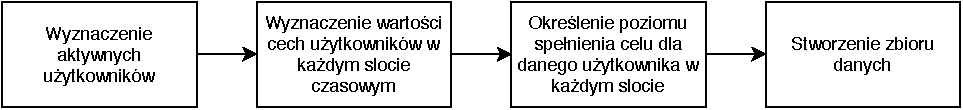
\includegraphics[width=150mm]{PracaMagisterska/Diagrams/dataset_preparation.pdf}
    \caption{Przygotowanie zbioru danych - diagram}
    \label{data_prep}
\end{figure}

    \FloatBarrier


Mając zbiór danych, strategie osiągania celów wyznaczę postępując według schematu widocznego na Rysunku~\ref{stat}.

 \begin{figure}[ht]
    \centering
    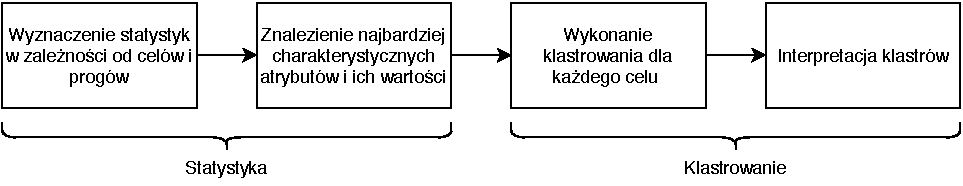
\includegraphics[width=150mm]{PracaMagisterska/Diagrams/stat.pdf}
    \caption{Znalezienie strategii - diagram}
    \label{stat}
\end{figure}

    \FloatBarrier

\begin{enumerate}
    \item \textbf{Statystyka}
    % \vspace{5mm}
    
    Każdy użytkownik w zbiorze danych posiada wartości cech jakie posiadał w danym slocie czasowym. Również posiada informacje na jakim poziomie osiągnął dany cel - popularność, wpływowość, relacje. Mając te dane, pogrupuję wszystkich użytkowników ze względu na poziom spełnienia danego celu, a następnie wyznaczę średnie, maksymalne, minimalne wartości cech oraz ich odchylenia standardowe. W rezultacie powinienem otrzymać cechy najbardziej charakterystyczne dla danego celu oraz ich wartości w dla poszczególnych poziomów. Cechy te zostaną wykorzystane do klastrowania osobno dla danego celu.
 
    
    \item \textbf{Klastrowanie}
    % \vspace{5mm}
    
    Klastrowanie służy do wyróżnienia grup danych o podobnych cechach. Mając wyznaczone poszczególne cechy dla każdego z trzech celów, sprawdzę czy po wykonaniu klasteryzacji, będzie można określić do jakiego klastra trafiają użytkownicy o danym poziomie spełnienia wybranego celu. Użyję algorytmu KMeans\cite{kmeans}, a w celu znalezienia optymalnej liczby klastrów użyję metody Elbow\cite{elbow}. Klasteryzacja będzie postępowała według schematu widocznego na Rysunku~\ref{cluster}:
    
     \begin{figure}[ht]
    \centering
    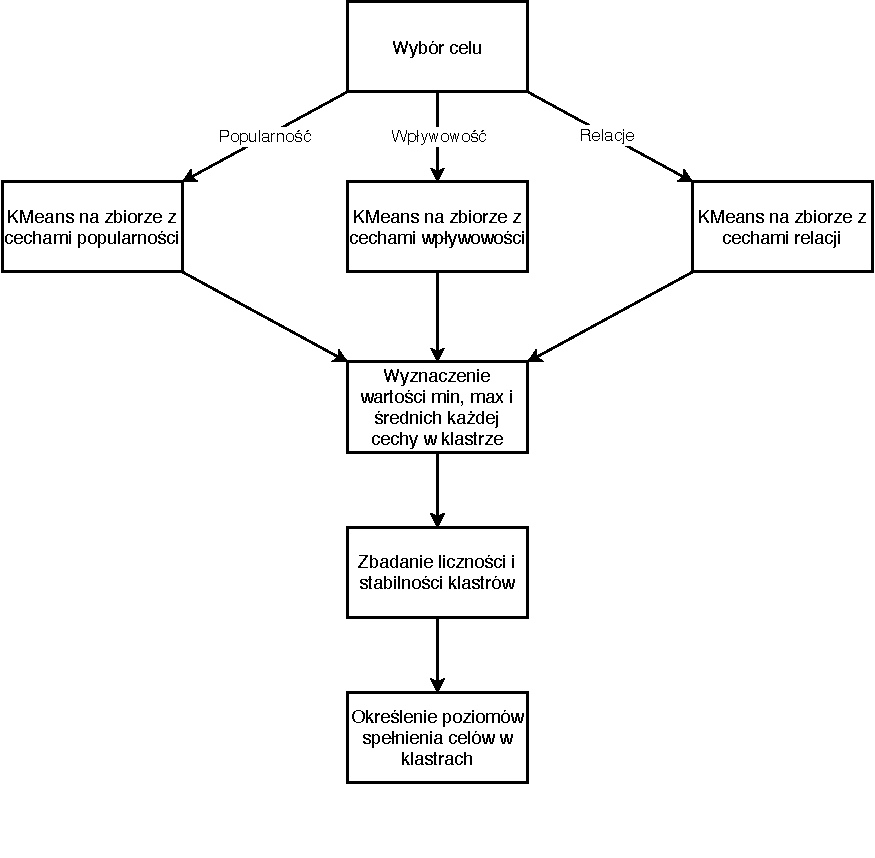
\includegraphics[width=150mm]{PracaMagisterska/Diagrams/cluster.pdf}
    \caption{Klasteryzacja - schemat działania}
    \label{cluster}
\end{figure}

    \FloatBarrier
\end{enumerate}




\subsection{Predykcja}

Kolejnym krokiem po wykonaniu klasteryzacji i znalezieniu cech, które wpływają na osiągnięcie danego celu, będzie wykonanie predykcji. Będę chciał sprawdzić z jaką skutecznością da się przewidzieć osiągnięcie danego celu przez użytkownika. Będę przewidywał poziom osiągnięcia celu, czyli np. dla popularności będę przewidywał, czy użytkownik osiągnie dużą, średnią, słabą popularność, albo czy nie osiągnie jej wcale. Miary są skonstruowane w taki sposób, że uwzględniają wcześniejsze wartości z poprzednich slotów z odpowiednimi wagami. Aby uniknąć zaburzeń predykcji z tym związanych, zamiast przewidywać, jaki poziom celu użytkownik osiągnie w kolejnym slocie czasowym, będę przewidywał poziom celu jaki osiągnie za pół roku. Do badań wybiorę dwa okresy czasowe: przed 2010 rokiem oraz po 2010 roku. W 2010 roku przybyło wiele nowych użytkowników i dynamicznie zmieniały się ich zachowania.

Zbadam również, jaki wpływ na wyniki ma długość historii użytkownika, którą wezmę pod uwagę. Minimalna długość jaką przyjmuję to 1 a maksymalna to 5. Na Rysunku~\ref{predic1} przedstawiona jest sytuacja, gdzie na podstawie jednego slotu (pomarańczowy kolor) przewidywane są poziomy osiągnięcia celów za pół roku (zielony kolor). Z kolej Rysunek~\ref{predic5} przedstawia scenariusz, w którym predykujemy na podstawie pięciu miesięcy. Wtedy wektor cech każdego użytkownika zawiera poszczególne cechy z badanych slotów. Dla celu popularność użytkownik jest opisany poprzez 6 cech. W przypadku brania pod uwagę historii jego działania o długości 5, jak na Rysunku~\ref{predic5}, wektor cech będzie miał długość 6*5 = 30. Wydłużanie długości historii powinno dać lepsze rezultaty predykcji.

     \begin{figure}[ht]
    \centering
    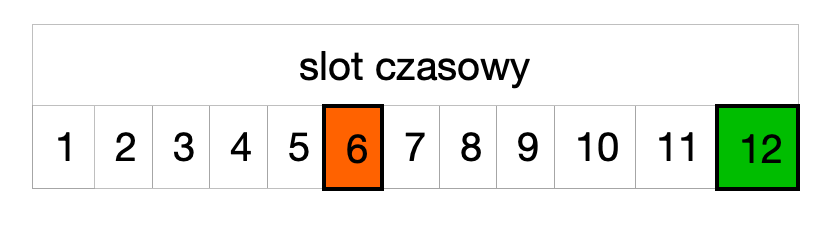
\includegraphics[width=100mm]{PracaMagisterska/Diagrams/slot1.png}
    \caption{Predykcja - 1 slot czasowy brany pod uwagę}
    \label{predic1}
\end{figure}

    \FloatBarrier


     \begin{figure}[ht]
    \centering
    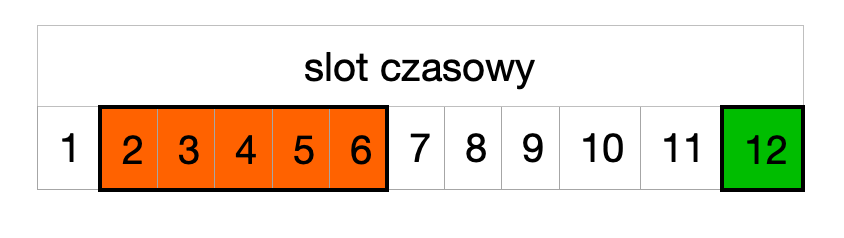
\includegraphics[width=100mm]{PracaMagisterska/Diagrams/sl.png}
    \caption{Predykcja - 5 slotów czasowych branych pod uwagę}
    \label{predic5}
\end{figure}

    \FloatBarrier



Wykorzystam następujące klasyfikatory: Naiwny klasyfikator bayesowski, drzewo decyzyjne (zoptymalizowana wersja CART), AdaBoost, las losowy oraz perceptron wielowarstwowy, które są opisane w rozdziale 2.5.1.

Miarami jakie wykorzystam do określenia jakości predykcji będą: precyzja ($precision$), czułość ($recall$) oraz $F_{1} score$ opisane wcześniej.

W zbiorze danych w znacznym stopniu przeważają użytkownicy nieosiągający danego celu, dlatego losowo usunę część z nich uzyskując mniejszą liczność tego zbioru. Następnie wykorzystam metodę dodającą próbki do mniej licznych klas (oversampling) i w rezultacie wszystkie cztery klasy będą podobnej liczności.


\newpage
\section{Wybrane aspekty realizacji}
\emph{W tym rozdziale przedstawię narzędzia wykorzystane w tym projekcie, architekturę i organizację systemu oraz opiszę bazę danych, z której dane były wykorzystywane}

\subsection{Narzędzia}
Wykorzystałem następujące narzędzia i pakiety:

\begin{itemize}
    \item \textbf{Python 3.6} - wybrałem ten język, z uwagi na szeroką dostępność bibliotek do analizy danych oraz uczenia maszynowego.
    \item \textbf{PostgreSQL} - relacyjna baza danych. Do pracy z bazą wykorzystałem narzędzie \textbf{pgAdmin 4}, które ułatwiło analizę danych w bazie.
    \item \textbf{scikit-learn}\footnote{https://scikit-learn.org}, \textbf{pandas}\footnote{https://pandas.pydata.org}, \textbf{numpy}\footnote{https://numpy.org}, \textbf{imblearn}\footnote{https://imbalanced-learn.readthedocs.io} - biblioteki dla Pythona, które umożliwiły analizę danych z bazy, przygotowanie zbioru danych, klastrowanie oraz predykcję.
    \item \textbf{PyCharm} - środowisko programistyczne dla języka Python
\end{itemize}


\subsection{Realizacja systemu}


    
Zastosowałem następującą architekturę, widoczną na Rysunku~\ref{architecture}. 

     \begin{figure}[ht]
    \centering
    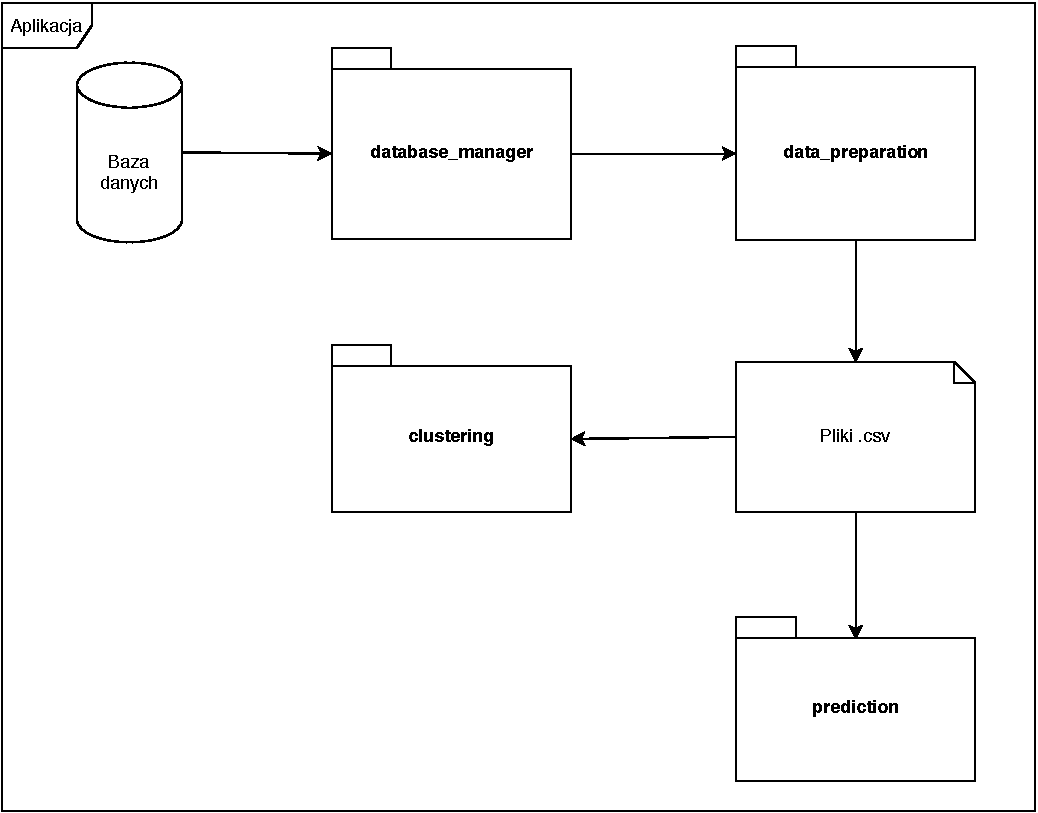
\includegraphics[width=150mm]{PracaMagisterska/Diagrams/architecture.pdf}
    \caption{Poglądowa architektura systemu}
    \label{architecture}
\end{figure}

  
    
Opis modułów:
\begin{itemize}
    \item \textbf{moduł database\_manager}
    
    Moduł ten odpowiada za komunikację z bazą danych. Komunikacja została zapewniona przez bibliotekę \textit{psycopg2}\footnote{https://www.psycopg.org}, dzięki której można było przekazywać zapytania do bazy danych. Aby nie pobierać informacji za każdym razem, ponieważ byłoby to zbyt czasochłonne, utworzyłem odpowiednie zapytania i ich wyniki zapisałem do plików w odpowiednich strukturach.
    
    \item \textbf{moduł data\_preparation}
    
    W tym module odbywają się wszystkie analizy danych pobranych z bazy. Wyznaczane są wartości metryk dla każdego celu i użytkownika. Grupowane są dane w odpowiednie struktury i finalnie tworzone pliki .csv, które są wykorzystywane do klastrowania i predykcji. W tym module korzystałem głównie z bibliotek \textit{pandas} oraz \textit{numpy}. 
    
    \item \textbf{moduł clustering}
    
    Ten moduł odpowiada za wykonanie klasteryzacji na odpowiednich zbiorach oraz zebranie wyników w postaci wykresów i wartości liczbowych. Algorytmy są inicjalizowane domyślnymi wartościami, zmianie ulega liczba klastrów w zależności od badanego celu. Domyślna konfiguracja wygląda następująco:
    

    
    \begin{itemize}
    \setlength\itemsep{0,1em}
    \item[--] init = k-means++ - centra klastrów inicjalizowane są tak, by jak najszybciej osiągnąć zbieżność. Innymi możliwościami jest np. inicjalizowanie centrów klastrów zadaną tablicą lub wybranie ich losowo.
    
    \item[--] n\_init = 10 - ilość wywołań algorytmu z różnymi centrami. Wybierane jest to wywołanie, które dało najlepsze rezultaty.
    
    \item[--] max\_iter = 300 - maksymalna liczba iteracji dla pojedynczego wywołania.
    
    \item[--] algorithm = auto - w tym przypadku jest to algorytm \textit{elkan}, który wykorzystuje nierówność trójkąta.

\end{itemize}
    
    \item \textbf{moduł prediction}
    
    Moduł odpowiedzialny za przeprowadzenie eksperymentów na zbiorach danych. Klasa \textit{MachineLearning()} jest konfigurowana za pomocą pliku, w którym określam dla jakiego celu ma zostać wykonana predykcja oraz czy zmodyfikować zbiory danych wykorzystując metody under- i oversamplingu. Po uruchomieniu klasy przygotowywane są struktury słownikowe, do których zapisywane są wyniki otrzymane przez poszczególne klasyfikatory, które są następnie wizualizowane. 
    
    Wykorzystane klasyfikatory posiadają następujące konfiguracje:
    \begin{enumerate}
        \item ComplementNB (Complement Naive Bayes\footnote{https://scikit-learn.org/stable/modules/naive\_bayes.html\#complement-naive-bayes}):
            \begin{itemize}
                \setlength\itemsep{0,1em}
                \item[--] alpha = 1.0 -  wygładzanie Laplace'a dla danych kategorycznych, gdzie wartość 0 to brak wygładzania.
                
                \item[--] class\_prior = None - służy do narzucenia prawdopodobieństwa występowania danej klasy.
                
                \item[--] norm = False - parametr mówiący o tym, czy ma zostać wykonana normalizacja wag.
            \end{itemize}
        
        \item DecisionTreeClassifier\footnote{https://scikit-learn.org/stable/modules/tree.html\#tree}:

            \begin{itemize}
                \setlength\itemsep{0,1em}
                \item[--] criterion = gini - funkcja mierząca jakość podziału.
                
                \item[--] splitter = best - strategia służąca do wyboru podziału dla węzła. Może być wybrana najlepsza, bądź losowa.
                
                \item[--] min\_samples\_split = 2 - minimalna liczba próbek wymagana do podzielenia węzła wewnętrznego.
                
                \item[--] min\_samples\_leaf = 1 - minimalna liczba próbek, która musi znajdować się w liścu.
            \end{itemize}
            
            Pozostałe parametry takie, jak maksymalna liczba w drzewie, czy też wagi klas nie są ustawiane.
            
        \item AdaBoostClassifier\footnote{https://scikit-learn.org/stable/modules/ensemble.html\#adaboost}:
            
            \begin{itemize}
                \setlength\itemsep{0,1em}
                \item[--] n\_estimators = 50 - maksymalna liczba estymatorów, przy której boosting jest przerywany.
                
                \item[--] learning\_rate = 1.0 - wskaźnik uczenia zmniejsza udział każdego klasyfikatora.
                
                \item[--] algorithm = SAMME.R 
            \end{itemize}
            
        \item RandomForestClassifier\footnote{https://scikit-learn.org/stable/modules/ensemble.html\#forest}:
            Posiada konfigurację, jak DecisionTreeClassifier oraz dodatkowe parametry:
            
            \begin{itemize}
                \setlength\itemsep{0,1em}
                \item[--] n\_estimators = 100 - liczba drzew w lesie.
                \item[--] bootstrap = True
            \end{itemize}
        
        \item MLPClassifier\footnote{https://scikit-learn.org/stable/modules/generated/sklearn.neural\_network.MLPClassifier.html}:
        
        \begin{itemize}
                \setlength\itemsep{0,1em}
                \item[--] hidden\_layer\_sizes = (100, )
                \item[--] activation = relu
                \item[--] solver = adam
                \item[--] alpha = 0.0001
                \item[--] learning\_rate = constant
                \item[--] learning\_rate\_init = 0.001
                \item[--] epsilon = 1e-08
            \end{itemize}
    \end{enumerate}
\end{itemize}

\subsection{Baza danych}

W pracy skorzystam ze zbioru danych z portalu Salon24. Zawiera on posty i komentarze użytkowników z okresu 1.01.2008 - 6.07.2013 dotyczące
ówczesnych wydarzeń i polityki. W zbiorze znajduje się 380700 postów, 5703140 komentarzy, 31750 autorów, a także informacje o tematach i użytych tagach. Dane przechowywane są w postaci relacyjnej bazy danych. Zawiera ona 8 tabel, natomiast nie wszystkie informacje są przydatne z punktu widzenia mojej pracy, dlatego wykorzystam następujące tabele i kolumny:
\begin{itemize}
    \item \textbf{Posts} - tabela zawiera posty pisane przez użytkowników portalu. Ich treść nie jest dla mnie interesująca, tylko informacje takie, jak:
        \begin{itemize}
            \item Id - identyfikator postu
            \item AutorId - identyfikator użytkownika, który napisał dany post
            \item Data - data utworzenia postu wraz z godziną

        \end{itemize}
    \item \textbf{Authors} - tabela zawiera dane o użytkownikach portalu. Wykorzystam następujące informacje:
    \begin{itemize}
            \item Id - identyfikator użytkownika
            \item Name - nazwa użytkownika w portalu

        \end{itemize}
    
    \item \textbf{Comments} - komentarze umieszczane pod postami innych. użytkowników. Wykorzystam następujące atrybuty:
    \begin{itemize}
            \item Id - identyfikator komentarza
            \item AutorId - identyfikator użytkownika, który napisał dany komentarz
            \item Data - data utworzenia komentarza wraz z godziną
            \item PostId - identyfikator postu, pod którym zamieszczono komentarz
            \item ParentCommentId - identyfikator nadrzędnego komentarza. Jeśli komentarz odnosi się do postu, wtedy ten atrybut ma wartość \textit{Null}
        \end{itemize}
\end{itemize}



\newpage
\section{Analiza zbioru danych}
\emph{Celem analizy zbioru danych jest przeprowadzenie badań pod kątem przedstawionych miar osiągania celów. Wynikiem analizy w tym rozdziale będą progi, określające uzyskanie danego celu przez użytkownika na danym poziomie.}




\subsection{Użytkownicy}

W zbiorze danych jest 31750 użytkowników. Są to użytkownicy, którzy byli aktywni na portalu, czyli dodali co najmniej jeden post lub komentarz. Możemy ich podzielić na trzy grupy: 

\begin{enumerate}
    \item autorzy postów - 10131 użytkowników
    \item autorzy komentarzy - 21619 użytkowników
    \item autorzy postów, którzy pisali komentarze - 7917 użytkowników
\end{enumerate}{}

Rysunek~\ref{fig:users_by_month} przedstawia przyrost użytkowników na przestrzeni lat. 
Możemy zobaczyć, że największy przyrost użytkowników miał miejsce w pierwszej połowie 2010 roku. Natomiast liczba aktywnych użytkowników w danym miesiącu jest przedstawiona na Rysunku~\ref{fig:active_users_by_month}. 

\begin{figure}[ht]
    \centering
    \includegraphics[width=0.8\textwidth]{users_by_month.png}
    \caption{Przyrost liczby użytkowników na portalu}
    \label{fig:users_by_month}
\end{figure}

\begin{figure}[ht]
    \centering
    \includegraphics[width=0.8\textwidth]{active_users_by_month.png}
    \caption[Liczba aktywnych użytkowników w miesiącu]{Liczba aktywnych użytkowników w danym miesiącu. Największą liczbę aktywnych użytkowników zanotowano na portalu Salon24 w latach 2010 i 2011.}
    \label{fig:active_users_by_month}
\end{figure}



Dane na temat aktywnych użytkowników będą mi potrzebne do wyznaczania miar popularności i wpływowości.


\subsection{Znajdowanie popularnych użytkowników}
Do znalezienia popularnych użytkowników wykorzystałem wcześniej wspomnianą metrykę \textit{Acquaintance Score}.

Do wyznaczenia miary uwzględnione zostały wszystkie interakcje pod postami danego użytkownika, włącznie z odpowiedziami na komentarze umieszczone przez innych. Czyli do tej metryki brane są pod uwagę wszystkie dyskusje toczone pod postami autora, które nie koniecznie odnoszą się już do autora postu.

 Tabela~\ref{tab1} przedstawia 10 najbardziej popularnych użytkowników według metryki \textit{Acquaintance Score}.
Popularność tych użytkowników była wyznaczana dla całego zbioru, czyli licznik w tej metryce to liczba uzyskanych interakcji w ciągu ponad 5 lat, natomiast mianownik to liczba użytkowników w zbiorze danych, czyli 31750. 



   
 \begin{table}

    \begin{center}
    

\begin{tabular}{ |c|c|c| } 
\hline
 \textbf{Lp} & \textbf{Użytkownik} & \textbf{Popularność} \\ [0.5ex] 
 \hline
 \hline
1 & FREE YOUR MIND & 4.79 \\
2 & RENATA RUDECKA-KALINOWSKA & 3.56 \\
3 & KRZYSZTOF LESKI & 3.32 \\
4 & CEZARY KRYSZTOPA & 2.67 \\
5 & SOWINIEC & 2.40 \\
6 & STARY & 2.16 \\
7 & GRZEGORZ WSZOŁEK - GW1990 & 2.14 \\
8 & UFKA & 2.14 \\
9 & MAREK MIGALSKI & 1.94 \\
10 & 1MAUD & 1.84 \\
 \hline
\end{tabular}
\end{center}
\caption[Popularni użytkownicy - wszystkie interakcje]{TOP10 popularnych użytkowników, biorąc pod uwagę wszystkie interakcje pod postami}
\label{tab1}
\end{table}

\FloatBarrier



To, jak się kształtowała popularność powyższych pięciu użytkowników przedstawione zostało na Rysunkach~\ref{fig:popularity_by_month} oraz ~\ref{fig:popularity_by_month_weighted}. W pierwszym przypadku wyznaczana jest popularność w oparciu o aktualny slot czasowy.



\begin{figure}[ht]
    \centering
    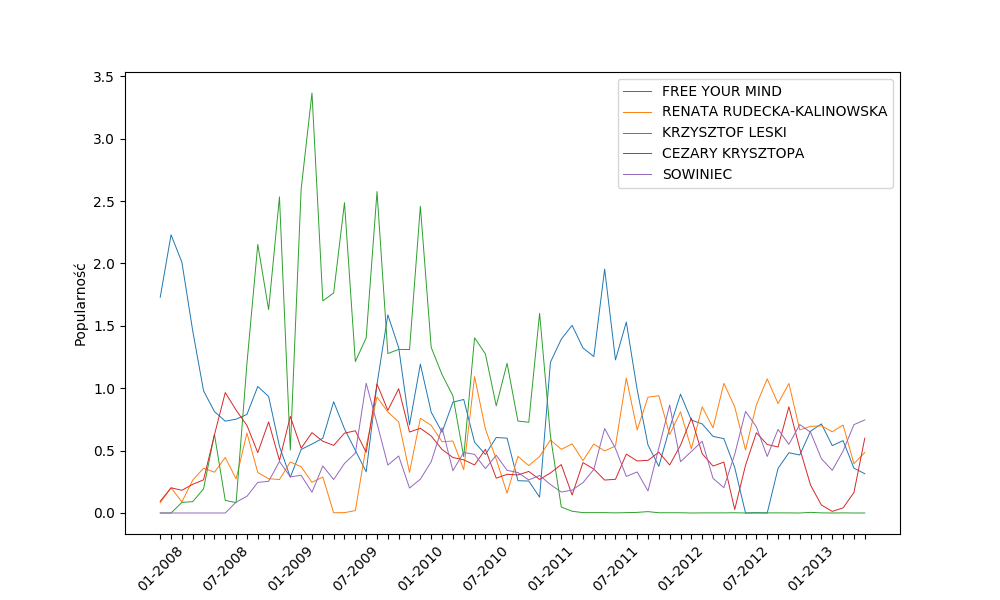
\includegraphics[width=0.8\textwidth]{active_popular_users.png}
    \caption[Popularność miesięczna - wszystkie interakcje]{Popularność miesięczna, w której uwzględniony jest tylko jeden badany slot czasowy}
    \label{fig:popularity_by_month}
\end{figure}



Na Rysunku~\ref{fig:popularity_by_month_weighted}, w którym brana jest pod uwagę popularność użytkownika w poprzednich slotach czasowych, widzimy, że popularność danego autora przyjmuje niższe wartości, ale utrzymuje się dłużej, nawet jeśli nie był on aktywny w późniejszym okresie.

\begin{figure}[ht]
    \centering
    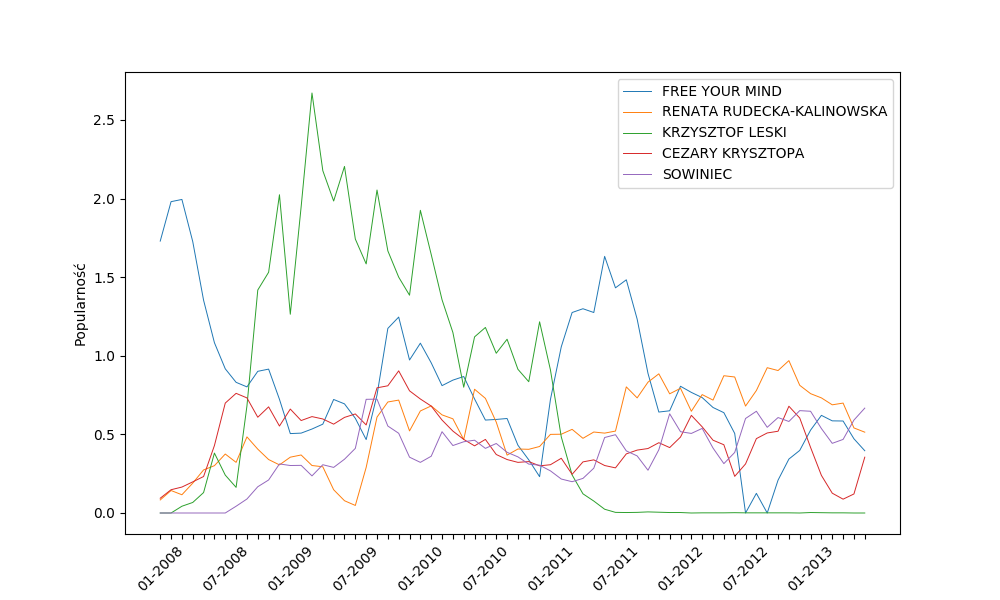
\includegraphics[width=0.8\textwidth]{all_weighted_fix.png}
    \caption[Popularność miesięczna - wszystkie interakcje - wagi]{Popularność miesięczna, w której uwzględnione zostały wcześniejsze sloty czasowe z odpowiednimi wagami}
    \label{fig:popularity_by_month_weighted}
\end{figure}

\FloatBarrier

W celu zrozumienia, jak się rozkłada miara popularności wśród użytkowników portalu, przedstawię na Rysunku~\ref{fig:pop_hist_all} histogramy w skali logarytmicznej w wybranych miesiącach. Możemy na nich zobaczyć, że niewielka część użytkowników otrzymuje wskaźnik powyżej 0.5. Histogramy były tworzone w oparciu o miarę z uwzględnieniem wcześniejszych slotów czasowych z odpowiednimi wagami.

\begin{figure*}[ht]
        \centering
        \begin{subfigure}[b]{0.48\textwidth}
            \centering
            \includegraphics[width=\textwidth]{active_popularity_by_month_2009.png}
            \caption[]%
            {{\small Liczba aktywnych użytkowników - 1628, liczba użytkowników wziętych pod uwagę przez tę miarę - 529}}   
            \label{fig:pop_hist_all1}
        \end{subfigure}
        \hfill
        \begin{subfigure}[b]{0.48\textwidth}  
            \centering 
            \includegraphics[width=\textwidth]{active_popularity_by_month_2010.png}
            \caption[]%
            {{\small Liczba aktywnych użytkowników - 2299, liczba użytkowników wziętych pod uwagę przez tę miarę - 831}}    
            \label{fig:pop_hist_all2}
        \end{subfigure}
        \vskip\baselineskip
        \begin{subfigure}[b]{0.48\textwidth}   
            \centering 
            \includegraphics[width=\textwidth]{active_popularity_by_month_2011.png}
            \caption[]%
            {{\small Liczba aktywnych użytkowników - 4247, liczba użytkowników wziętych pod uwagę przez tę miarę - 1360}}    
            \label{fig:pop_hist_all3}
        \end{subfigure}
        \quad
        \begin{subfigure}[b]{0.48\textwidth}   
            \centering 
            \includegraphics[width=\textwidth]{active_popularity_by_month_2012.png}
            \caption[]%
            {{\small Liczba aktywnych użytkowników - 4066, liczba użytkowników wziętych pod uwagę przez tę miarę - 1477}}    
            \label{fig:pop_hist_all4}
        \end{subfigure}
        \caption[ Histogramy popularności w zależności od okresu czasowego - wszystkie bez odpowiedzi na komentarze]
        {\small Histogramy popularności w zależności od okresu czasowego. Dla każdego z histogramów została podana liczba aktywnych użytkowników, która była brana pod uwagę, przy wyliczaniu miary popularności} 
        \label{fig:pop_hist_all}
    \end{figure*}
    
\FloatBarrier
    



\noindent
\textbf{Wnioski}

Na podstawie dokonanej analizy postanowiłem ustalić progi popularności. Przedstawiają się one następująco:

\begin{table}[h]
\centering
\begin{tabular}{|c|c|}
\hline
Brak popularności & 0 - 0.05 \\
\hline
Słaba popularność & 0.05 - 0.12 \\
\hline
Średnia popularność & 0.12 - 0.3 \\
\hline
Duża popularność & powyżej 0.3 \\
\hline
\end{tabular}
\caption[Progi popularności]{Progi popularności}
\label{tab:progi_popul}
\end{table}

Na Rysunku~\ref{fig:active_popularity_count} przedstawiłem, jak kształtuje się liczba popularnych użytkowników w zależności od progu i czasu. Znalezieni użytkownicy posłużą do wyznaczenia optymalnych strategii, które sprawiły, że uzyskali oni taki stopień popularności.

\begin{figure}[!htbp]
    \centering
    \includegraphics[width=0.8\textwidth]{active_popularity_by_month_user_count.png}
    \caption{Liczba użytkowników według progów popularności - wszystkie interakcje}
    \label{fig:active_popularity_count}
\end{figure}



\FloatBarrier

Tabela~\ref{tab:popul_count} przedstawia średnią liczbę użytkowników, którzy osiągnęli dany próg. Jest to średnia miesięczna.

\begin{table}[h]
\centering
\begin{tabular}{|c|c|}
\hline
\textbf{Próg popularności} & \textbf{Średnia liczba użytkowników} \\
\hline
Słaba popularność & 69 \\
\hline
Średnia popularność & 36 \\
\hline
Duża popularność & 16 \\
\hline
\end{tabular}
\caption{Średnia liczba użytkowników w danym progu}
\label{tab:popul_count}
\end{table}

\FloatBarrier



\subsection{Znajdowanie wpływowych użytkowników}

Wpływowych użytkowników wyszukuję na podstawie miary opisanej wzorem~\ref{n20}. W Tabeli~\ref{tab:inf} przedstawionych 10-ciu najbardziej wpływowych użytkowników według tej miary. Widać różnicę w porównaniu z użytkownikami, którzy są najbardziej popularni. Zostali oni wyznaczeni również w oparciu o cały zbiór danych, nie uwzględniając dynamiki.

\vspace{5mm}

\begin{table}[h]
\centering
  
\begin{tabular}{ |c|c|c| } 
\hline
 \textbf{Lp} & \textbf{Użytkownik} & \textbf{Wpływowość} \\ [0.5ex] 
 \hline
 \hline     
1 & JAN POSPIESZALSKI & 27.13 \\
2 & ERNEST SKALSKI & 25.77 \\
3 & KAZIMIERZ WÓYCICKI & 25.27 \\
4 & PUBLICYŚCI RZECZPOSPOLITEJ & 24.94 \\
5 & D. ARCISZEWSKA-MIELEWCZYK & 24.52 \\
6 & TOMASZ SAKIEWICZ & 22.5 \\
7 & FORUM ŻYDÓW POLSKICH & 22.47 \\
8 & JFLIBICKI & 20.65 \\
9 & KRZYSZTOF RYBIŃSKI & 20.5 \\
10 & M. J. CHODAKIEWICZ & 20.13 \\
  \hline
\end{tabular}
\caption{TOP 10 najbardziej wpływowych użytkowników portalu Salon24 wg miary wpływowości}
\label{tab:inf}
\end{table}


\begin{figure}[ht]
    \centering
    \includegraphics[width=0.8\textwidth]{influence_static.png}
    \caption[Wpływowi użytkownicy - histogram]{Histogram przedstawiający rozkład miary wpływowości}
    \label{fig:influence_static}
\end{figure}

\FloatBarrier

\textbf{Wnioski}

\vspace{5mm}

Na podstawie otrzymanych wyników zdefiniowałem progi wpływowości, które widoczne są w Tabeli~\ref{tab:progi_inf}.

\begin{table}[h]
\centering
\begin{tabular}{|c|c|}
\hline
Brak wpływowości & 0 - 2 \\
\hline
Słaba wpływowość & 2 - 5 \\
\hline
Średnia wpływowość & 5 - 15 \\
\hline
Duża wpływowość & powyżej 15 \\
\hline
\end{tabular}
\caption[Progi wpływowości]{Progi wpływowości}
\label{tab:progi_inf}
\end{table}

Na Rysunku~\ref{fig:inf_count} przedstawiłem, jak zmienia się liczba wpływowych użytkowników podzielonych według progów na przestrzeni miesięcy. Do policzenia miar w poszczególnych miesiącach uwzględniłem także dane o wpływowości z poprzednich slotów czasowych z odpowiednimi wagami.

\begin{figure}[ht]
    \centering
    \includegraphics[width=0.8\textwidth]{influence_count.png}
    \caption[Liczba wpływowych użytkowników wg progów na przestrzeni miesięcy]{Liczba wpływowych użytkowników wg progów na przestrzeni miesięcy}
    \label{fig:inf_count}
\end{figure}

\FloatBarrier

Tabela~\ref{tab:popul_count2} przedstawia średnią liczbę użytkowników, którzy osiągnęli dany próg. Jest to średnia miesięczna.

\begin{table}[h]
\centering
\begin{tabular}{|c|c|}
\hline
\textbf{Próg wpływowości} & \textbf{Średnia liczba użytkowników} \\
\hline
Słaba wpływowość & 73 \\
\hline
Średnia wpływowość & 31 \\
\hline
Duża wpływowość & 11 \\
\hline
\end{tabular}
\caption{Średnia liczba użytkowników w danym progu}
\label{tab:popul_count2}
\end{table}

\FloatBarrier



\subsection{Relacje między użytkownikami}

Związki między użytkownikami są istotnym punktem moich badań. Użytkownicy nawiązując silne relacje mogą również uzyskać popularność czy też wpływowość, jeśli będą w stałej relacji z popularną osobą.


Relacja użytkowników będzie wyznaczana w oparciu o komentarze zamieszczane do postów.

Prześledzę najpierw, jak na przestrzeni miesięcy zmieniała się liczba zamieszczanych komentarzy przez użytkowników. Na Rysunku~\ref{fig:comments_count} możemy to zobaczyć z podziałem na komentarze napisane bezpośrednio do posta, jak i komentarze będące odpowiedzią na inny komentarz.

\begin{figure}[ht]
    \centering
    \includegraphics[width=0.8\textwidth]{comment_frequency.png}
    \caption{Liczba komentarzy w zależności od miesiąca}
    \label{fig:comments_count}
\end{figure}

\FloatBarrier

Z wykresu wynika, że przez pierwszy rok dominowały bezpośrednie komentarze zamieszczane pod postami, natomiast w 2010 roku ta tendencja się odwróciła i większość komentarzy stanowiły odpowiedzi na komentarze pozostałych użytkowników. W moich analizach będę jednak wykorzystywał komentarze, które były bezpośrednio zamieszczane do postów.

Analizując zbiór danych, znalazłem użytkowników, którzy posiadali wysoki wskaźnik wzajemnie komentowanych postów. Są to użytkownicy Sowiniec oraz Godziemba. Rysunek~\ref{fig:sowiniecgodz} przedstawia stosunek liczby komentarzy otrzymanych przez użytkownika do liczby postów zamieszczonych w danym slocie czasowym. Z tego wynika, że Sowiniec komentował prawie każdy post użytkownika Godziemba. 

\begin{figure}[ht]
    \centering
    \includegraphics[width=0.8\textwidth]{sowiniec_godziemba.png}
    \caption{Relacja Sowiniec - Godziemba}
    \label{fig:sowiniecgodz}
\end{figure}

\FloatBarrier

Rysunek~\ref{fig:relcount} przedstawia liczbę relacji wśród użytkowników portalu, którzy zamieścili więcej niż 100 postów. Relacje zostały podzielone według progów z Tabeli~\ref{tab:tab_relacje}. Jest to relacja obustronna wyznaczana w taki sposób, że użytkownicy muszą wzajemnie skomentować określony procent postów. Z histogramu wynika, że jest niewielka liczba relacji, które są bardzo silne.

\begin{figure}[ht]
    \centering
    \includegraphics[width=0.8\textwidth]{relation_count_post.png}
    \caption{Liczba relacji wśród użytkowników portalu}
    \label{fig:relcount}
\end{figure}

\FloatBarrier


Na podstawie otrzymanych wyników ustaliłem następujące progi relacji widoczne w Tabeli~\ref{tab:rel_progi}.

\begin{table}[h]
\centering
\begin{tabular}{|c|c|}
\hline
Brak relacji & 0  \\
\hline
Słaba relacja & 1 - 2 \\
\hline
Średnia siła relacji & 3 - 4 \\
\hline
Silna relacja & 5 - 10 \\
\hline
\end{tabular}
\caption[Progi siły relacji]{Progi siły relacji}
\label{tab:rel_progi}
\end{table}

\begin{figure}[ht]
    \centering
    \includegraphics[width=0.8\textwidth]{relation_count_fix_5_weak_relation.png}
    \caption[Liczby słabych relacji]{Liczby słabych relacji na przestrzeni miesięcy z podziałem na poszczególne poziomy}
    \label{fig:weak_relation_count}
\end{figure}

\FloatBarrier

\begin{figure}[ht]
    \centering
    \includegraphics[width=0.8\textwidth]{relation_count_fix_5_avg_relation.png}
    \caption[Liczby relacji o średniej sile]{Liczby relacji o średniej sile na przestrzeni miesięcy z podziałem na poszczególne poziomy}
    \label{fig:avg_relation_count}
\end{figure}

\FloatBarrier

\begin{figure}[ht]
    \centering
    \includegraphics[width=0.8\textwidth]{relation_count_fix_5_strong_relation.png}
    \caption[Liczby silnych relacji]{Liczby silnych relacji na przestrzeni miesięcy z podziałem na poszczególne poziomy}
    \label{fig:strong_relation_count}
\end{figure}

\FloatBarrier

Tabela~\ref{tab:rel_count2} przedstawia średnią liczbę relacji, które osiągnęły dany próg. Jest to średnia miesięczna.

\begin{table}[h]
\centering
\begin{tabular}{|c|c|}
\hline
\textbf{Próg relacji} & \textbf{Średnia liczba relacji} \\
\hline
Słaba relacja & 3638 \\
\hline
Średnia siła relacji & 51 \\
\hline
Silna relacja & 8 \\
\hline
\end{tabular}
\caption{Średnia liczba relacji w danym progu}
\label{tab:rel_count2}
\end{table}

\FloatBarrier

Z punktu widzenia danych jakie posiadam i jak je będę wykorzystywał do klastrowania i predykcji, potrzebuję określić jaki poziom relacji udało się osiągnąć danemu użytkownikowi w danym slocie czasowym. Przykładowo, jeśli użytkownik osiągnął co najmniej jedną silną relację w slocie czasowym, to znaczy że posiada cechy umożliwiające mu osiągnięcie tego celu na tym poziomie.

\begin{figure}[ht]
    \centering
    \includegraphics[width=0.8\textwidth]{relation_count.png}
    \caption{Liczba użytkowników, którzy osiągnęli relację na danym poziomie na przestrzeni miesięcy}
    \label{fig:rel_count}
\end{figure}

\FloatBarrier

Tabela~\ref{tab:relation_count2} przedstawia średnią liczbę użytkowników, którzy osiągnęli dany próg. Jest to średnia miesięczna.

\begin{table}[h]
\centering
\begin{tabular}{|c|c|}
\hline
\textbf{Próg relacji} & \textbf{Średnia liczba użytkowników} \\
\hline
Słaba relacja & 120 \\
\hline
Średnia siła relacji & 22 \\
\hline
Silna relacja & 4 \\
\hline
\end{tabular}
\caption{Średnia liczba użytkowników w danym progu}
\label{tab:relation_count2}
\end{table}

\FloatBarrier


\newpage
\section{Eksperymenty i wyniki}
\emph{W tym rozdziale znalezieni zostaną aktywni użytkownicy, którzy zostaną wzięci pod uwagę w kolejnych krokach. Mając określone poziomy spełnienia danego celu i przygotowany zbiór danych sprawdzę, jakie wartości cech uzyskiwali użytkownicy na danym poziomie. Następnie wykonam klasteryzację dla danego celu uwzględniając wybrane cechy. Na końcu sprawdzę, czy na podstawie wybranych cech można przewidzieć poziom osiągnięcia danego celu przez użytkownika w przyszłości.}

\subsection{Znalezienie aktywnych użytkowników}
Zgodnie z opisem w punkcie 3.4.1, ze zbioru użytkowników, zostaną odrzuceni ci, którzy nie byli wystarczająco aktywni. Po zsumowaniu wszystkich wpisów użytkowników na portalu stworzyłem histogram widoczny na Rysunku ~\ref{fig:hist_active} przedstawiający rozkład wpisów użytkowników.

\begin{figure}[ht]
    \centering
    \includegraphics[width=0.8\textwidth]{user_interactions.png}
    \caption{Histogram - rozkład wpisów użytkowników}
    \label{fig:hist_active}
\end{figure}

\FloatBarrier

Znaczna większość użytkowników, to ci, którzy nie spełnili kryterium i zostali usunięci ze zbioru danych. Z 31750 użytkowników, zostało 5704, którzy byli aktywni i oni zostaną poddani dalszej analizie.

\subsection{Statystyczne wyznaczenie wartości cech dla danego celu}

Postępując zgodnie ze schematem opisanym na Rysunku~\ref{data_prep} stworzyłem zbiór danych. Każdy z 5704 znajdujących się w nim użytkowników jest opisany poprzez zestaw 11 cech na przestrzeni 65 slotów czasowych. Dodatkowo każdy użytkownik ma przypisany osiągnięty poziom celów: popularności, wpływowości oraz osiągnięcia relacji. W tym podrozdziale pogrupowałem zbiór danych po poziomie osiągnięcia danego celu. Pozwoliło mi to określić szczególne cechy oraz ich wartości dla danego poziomu.

\subsubsection{Popularność}

Popularność zależy od liczby interakcji otrzymanych pod napisanymi postami, a także od liczby aktywnych użytkowników w danym miesiącu. Wybierając ostateczne cechy, odrzucę te, które są najbardziej skorelowane z miarą. W tym przypadku cecha \textit{user\_interaction\_received} jest najbardziej związana z miarą popularności. W Tabelach~\ref{tab:pp0}, ~\ref{tab:pp1}, ~\ref{tab:pp2} oraz ~\ref{tab:pp3} przedstawione wartości minimalne, średnie, odchylenia standardowe oraz wartości maksymalne dla każdej cechy w zależności od poziomu popularności.


\begin{table}[ht]
    \centering
  \begin{center}
  \begin{tabular}{|c|c|c|c|c|}
  \hline
  Cecha & Min & Średnia & Std & Max  \\
  \hline
post\_written & 0.0 & 1.77 & 4.58 & 191.0 \\
\hline
comments\_noreply\_written & 0.0 & 15.74 & 34.52 & 1111.0 \\
\hline
comments\_reply\_written & 0.0 & 13.76 & 36.54 & 1712.0 \\
\hline
post\_interaction\_count & 0.0 & 1.37 & 3.94 & 216.0 \\
\hline
comment\_interaction\_count & 0.0 & 1.15 & 2.13 & 87.0 \\
\hline
interacted\_with & 0.0 & 9.56 & 15.96 & 336.0 \\
\hline
user\_interaction\_received & 0.0 & 4.01 & 9.89 & 166.0 \\
\hline
interacted\_with\_last\_slot\_percentage & 0.0 & 18.02 & 26.67 & 100.0 \\
\hline
user\_interaction\_received\_last\_slot\_percentage & 0.0 & 2.65 & 9.9 & 100.0 \\
\hline
relations\_count\_with\_popular & 0.0 & 0.05 & 0.37 & 21.0 \\
\hline
relations\_count\_with\_influential & 0.0 & 0.02 & 0.21 & 20.0 \\
\hline
  \end{tabular}
\end{center}
\caption{Statystyki - brak popularności}
\label{tab:pp0}
\end{table}


\begin{table}[ht]
    \centering
  \begin{center}
  \begin{tabular}{|c|c|c|c|c|}
  \hline
  Cecha & Min & Średnia & Std & Max  \\
  \hline
post\_written & 0.0 & 13.18 & 13.04 & 220.0 \\
\hline
comments\_noreply\_written & 0.0 & 58.66 & 72.44 & 759.0 \\
\hline
comments\_reply\_written & 0.0 & 86.04 & 105.77 & 993.0 \\
\hline
post\_interaction\_count & 0.0 & 12.52 & 14.52 & 154.0 \\
\hline
comment\_interaction\_count & 0.0 & 2.35 & 3.89 & 69.0 \\
\hline
interacted\_with & 0.0 & 22.39 & 26.51 & 289.0 \\
\hline
user\_interaction\_received & 0.0 & 54.28 & 36.84 & 285.0 \\
\hline
interacted\_with\_last\_slot\_percentage & 0.0 & 32.36 & 24.62 & 100.0 \\
\hline
user\_interaction\_received\_last\_slot\_percentage & 0.0 & 22.81 & 14.92 & 100.0 \\
\hline
relations\_count\_with\_popular & 0.0 & 1.24 & 2.14 & 29.0 \\
\hline
relations\_count\_with\_influential & 0.0 & 0.34 & 1.08 & 23.0 \\
\hline
  \end{tabular}
\end{center}
\caption{Statystyki - słaba popularność}
\label{tab:pp1}
\end{table}


\begin{table}[ht]
    \centering
  \begin{center}
  \begin{tabular}{|c|c|c|c|c|}
  \hline
  Cecha & Min & Średnia & Std & Max  \\
  \hline
post\_written & 0.0 & 17.82 & 16.83 & 228.0 \\
\hline
comments\_noreply\_written & 0.0 & 105.14 & 124.43 & 1092.0 \\
\hline
comments\_reply\_written & 0.0 & 151.58 & 179.82 & 1371.0 \\
\hline
post\_interaction\_count & 0.0 & 19.63 & 20.81 & 248.0 \\
\hline
comment\_interaction\_count & 0.0 & 3.03 & 5.22 & 88.0 \\
\hline
interacted\_with & 0.0 & 25.36 & 28.08 & 253.0 \\
\hline
user\_interaction\_received & 0.0 & 102.26 & 69.76 & 862.0 \\
\hline
interacted\_with\_last\_slot\_percentage & 0.0 & 36.63 & 23.79 & 100.0 \\
\hline
user\_interaction\_received\_last\_slot\_percentage & 0.0 & 30.62 & 12.45 & 100.0 \\
\hline
relations\_count\_with\_popular & 0.0 & 2.27 & 2.59 & 20.0 \\
\hline
relations\_count\_with\_influential & 0.0 & 0.43 & 1.09 & 9.0 \\
\hline
  \end{tabular}
\end{center}
\caption{Statystyki - średnia popularność}
\label{tab:pp2}
\end{table}


\begin{table}[ht]
    \centering
  \begin{center}
  \begin{tabular}{|c|c|c|c|c|}
  \hline
  Cecha & Min & Średnia & Std & Max  \\
  \hline
post\_written & 1.0 & 25.75 & 17.84 & 157.0 \\
\hline
comments\_noreply\_written & 0.0 & 229.24 & 269.01 & 2336.0 \\
\hline
comments\_reply\_written & 0.0 & 394.39 & 471.95 & 3400.0 \\
\hline
post\_interaction\_count & 4.44 & 28.21 & 25.07 & 291.5 \\
\hline
comment\_interaction\_count & 0.0 & 3.27 & 5.88 & 98.0 \\
\hline
interacted\_with & 0.0 & 34.93 & 40.76 & 255.0 \\
\hline
user\_interaction\_received & 12.0 & 200.02 & 121.81 & 733.0 \\
\hline
interacted\_with\_last\_slot\_percentage & 0.0 & 39.11 & 20.95 & 100.0 \\
\hline
user\_interaction\_received\_last\_slot\_percentage & 0.0 & 38.28 & 10.83 & 100.0 \\
\hline
relations\_count\_with\_popular & 0.0 & 4.13 & 4.38 & 37.0 \\
\hline
relations\_count\_with\_influential & 0.0 & 1.07 & 1.88 & 11.0 \\
\hline
  \end{tabular}
\end{center}
\caption{Statystyki - duża popularność}
\label{tab:pp3}
\end{table}

\FloatBarrier

Najbardziej charakterystyczne wartości osiągane są dla dużej popularności. Użytkownicy będący na tym poziomie piszą co najmniej jeden post w ciągu miesiąca, a średnia wartość wynosi ~26. Również liczby pisanych komentarzy się wyróżniają. Najbardziej popularni użytkownicy zamieszczają średnio 229 komentarzy pod postami, z kolei użytkownicy ze średnią popularnością zamieszczają ich 105, a ze słabą - 59. Cecha \textit{post\_interaction\_count} przyjmuje minimalną wartość niezerową tylko dla dużej popularności i wynosi 4.44. Znaczy to, że każdy napisany post otrzymał więcej niż 4 komentarze, a średnia wartość wynosi 25. Jeśli chodzi o liczbę komentarzy otrzymanych przypadających na jeden napisany, to różnice nie są już takie duże dla poszczególnych poziomów, ale największą wartość średnią i maksymalną otrzymano dla dużej popularności. Ci użytkownicy charakteryzują się również tym, że wchodzą w interakcje z wieloma różnymi osobami w ciągu miesiąca. Na popularność nie ma z kolei wpływu to z jakim procentem użytkowników utrzymywany jest "kontakt" w kolejnych slotach. Ostatnią cechą mogącą mieć wpływ na uzyskanie dużej popularności jest liczba nawiązywanych relacji z innymi popularnymi użytkownikami.

Do klastrowania wykorzystam następujące cechy:

\begin{itemize}
    \setlength\itemsep{0,005em}
    \item[--] post\_written
    \item[--] comments\_noreply\_written 
    \item[--] comments\_reply\_written
    \item[--] post\_interaction\_count
    \item[--] comment\_interaction\_count 
    \item[--] interacted\_with
    \item[--] relations\_count\_with\_popular 
\end{itemize}



\subsubsection{Wpływowość}

Wpływowości zależy od stosunku liczby otrzymanych komentarzy pod napisanymi postami i komentarzami. Dlatego nie będę skupiał się na cechach \textit{post\_interaction\_count} i \textit{comment\_interaction\_count}, ale znajdą się one w Tabelach~\ref{tab:ii0} -~\ref{tab:ii3}, żeby zobaczyć jakie wartości te cechy uzyskały. 


\begin{table}[ht]
    \centering
  \begin{center}
  \begin{tabular}{|c|c|c|c|c|}
  \hline
  Cecha & Min & Średnia & Std & Max  \\
  \hline
post\_written & 0.0 & 2.4 & 6.56 & 228.0 \\
\hline
comments\_noreply\_written & 0.0 & 21.32 & 53.32 & 2336.0 \\
\hline
comments\_reply\_written & 0.0 & 22.6 & 77.15 & 3400.0 \\
\hline
post\_interaction\_count & 0.0 & 1.54 & 4.48 & 266.4 \\
\hline
comment\_interaction\_count & 0.0 & 1.2 & 2.15 & 87.0 \\
\hline
interacted\_with & 0.0 & 10.94 & 17.82 & 336.0 \\
\hline
user\_interaction\_received & 0.0 & 6.35 & 21.03 & 701.0 \\
\hline
interacted\_with\_last\_slot\_percentage & 0.0 & 18.82 & 26.27 & 100.0 \\
\hline
user\_interaction\_received\_last\_slot\_percentage & 0.0 & 3.54 & 11.25 & 100.0 \\
\hline
relations\_count\_with\_popular & 0.0 & 0.14 & 0.85 & 29.0 \\
\hline
relations\_count\_with\_influential & 0.0 & 0.04 & 0.38 & 23.0 \\
\hline
  \end{tabular}
\end{center}
\caption{Statystyki - brak wpływowości}
\label{tab:ii0}
\end{table}

Analizując tabele można zobaczyć, że duża liczba pisanych postów nie wpływa na uzyskanie dużej wpływowości, a wręcz przeciwnie - najbardziej wpływowi użytkownicy posiadają najmniejsze wartości średnie i maksymalne liczby pisanych postów. Tak samo jest z komentarzami i liczbą różnych użytkowników, którym komentują posty. Użytkownikami piszącymi średnio najwięcej komentarzy, są ci co nie uzyskali wpływowości. Najbardziej wpływowi użytkownicy otrzymują natomiast średnio najwięcej komentarzy od różnych osób. Ta liczba wynosi 110, a maksymalna otrzymana wartość to 733. Jak można było zobaczyć w poprzednim rozdziale w Tabeli~\ref{tab:inf}, najbardziej wpływowi użytkownicy to głównie dziennikarze i publicyści, co tłumaczy wartości poszczególnych cech. Utrzymywanie kontaktów w kolejnych slotach w użytkownikami nie wpływa na osiągnięty poziom.


\begin{table}[ht]
    \centering
  \begin{center}
  \begin{tabular}{|c|c|c|c|c|}
  \hline
  Cecha & Min & Średnia & Std & Max  \\
  \hline
post\_written & 0.0 & 6.76 & 9.39 & 141.0 \\
\hline
comments\_noreply\_written & 0.0 & 9.56 & 31.14 & 688.0 \\
\hline
comments\_reply\_written & 0.0 & 11.22 & 44.39 & 1118.0 \\
\hline
post\_interaction\_count & 0.0 & 9.52 & 13.22 & 291.5 \\
\hline
comment\_interaction\_count & 0.0 & 1.66 & 3.48 & 51.0 \\
\hline
interacted\_with & 0.0 & 3.41 & 7.07 & 116.0 \\
\hline
user\_interaction\_received & 0.0 & 37.42 & 54.21 & 862.0 \\
\hline
interacted\_with\_last\_slot\_percentage & 0.0 & 22.6 & 33.7 & 100.0 \\
\hline
user\_interaction\_received\_last\_slot\_percentage & 0.0 & 11.6 & 14.91 & 100.0 \\
\hline
relations\_count\_with\_popular & 0.0 & 0.3 & 1.07 & 16.0 \\
\hline
relations\_count\_with\_influential & 0.0 & 0.05 & 0.33 & 8.0 \\
\hline
  \end{tabular}
\end{center}
\caption{Statystyki - słaba wpływowość}
\label{tab:ii1}
\end{table}


\begin{table}[ht]
    \centering
  \begin{center}
  \begin{tabular}{|c|c|c|c|c|}
  \hline
  Cecha & Min & Średnia & Std & Max  \\
  \hline
post\_written & 0.0 & 8.18 & 8.97 & 71.0 \\
\hline
comments\_noreply\_written & 0.0 & 6.51 & 17.93 & 333.0 \\
\hline
comments\_reply\_written & 0.0 & 7.19 & 17.39 & 236.0 \\
\hline
post\_interaction\_count & 0.0 & 21.84 & 21.99 & 233.0 \\
\hline
comment\_interaction\_count & 0.0 & 2.78 & 6.73 & 98.0 \\
\hline
interacted\_with & 0.0 & 2.14 & 4.33 & 64.0 \\
\hline
user\_interaction\_received & 0.0 & 85.17 & 95.43 & 672.0 \\
\hline
interacted\_with\_last\_slot\_percentage & 0.0 & 24.54 & 36.59 & 100.0 \\
\hline
user\_interaction\_received\_last\_slot\_percentage & 0.0 & 19.3 & 16.79 & 100.0 \\
\hline
relations\_count\_with\_popular & 0.0 & 0.87 & 2.11 & 37.0 \\
\hline
relations\_count\_with\_influential & 0.0 & 0.08 & 0.39 & 9.0 \\
\hline
  \end{tabular}
\end{center}
\caption{Statystyki - średnia wpływowość}
\label{tab:ii2}
\end{table}


\begin{table}[ht]
    \centering
  \begin{center}
  \begin{tabular}{|c|c|c|c|c|}
  \hline
  Cecha & Min & Średnia & Std & Max  \\
  \hline
post\_written & 0.0 & 6.12 & 7.55 & 42.0 \\
\hline
comments\_noreply\_written & 0.0 & 2.08 & 7.4 & 89.0 \\
\hline
comments\_reply\_written & 0.0 & 1.62 & 5.74 & 85.0 \\
\hline
post\_interaction\_count & 0.0 & 38.76 & 23.9 & 153.0 \\
\hline
comment\_interaction\_count & 0.0 & 2.23 & 5.88 & 71.0 \\
\hline
interacted\_with & 0.0 & 0.94 & 2.23 & 18.0 \\
\hline
user\_interaction\_received & 0.0 & 110.21 & 117.22 & 733.0 \\
\hline
interacted\_with\_last\_slot\_percentage & 0.0 & 17.09 & 34.58 & 100.0 \\
\hline
user\_interaction\_received\_last\_slot\_percentage & 0.0 & 20.94 & 16.08 & 100.0 \\
\hline
relations\_count\_with\_popular & 0.0 & 0.98 & 2.21 & 19.0 \\
\hline
relations\_count\_with\_influential & 0.0 & 0.06 & 0.28 & 4.0 \\
\hline
  \end{tabular}
\end{center}
\caption{Statystyki - duża wpływowość}
\label{tab:ii3}
\end{table}

\FloatBarrier

Do klastrowania wezmę pod uwagę następujące cechy:

\begin{itemize}
    \setlength\itemsep{0,005em}
    \item[--] post\_written
    \item[--] comments\_noreply\_written 
    \item[--] comments\_reply\_written
    \item[--] interacted\_with
    \item[--] user\_interaction\_received
    \item[--] relations\_count\_with\_influential
\end{itemize}


\subsubsection{Relacje}

Badając relacje skupię się głównie na cechach związanych z innymi użytkownikami. Jest to 6 ostatnich cech w każdej z Tabel~\ref{tab:rr0} -~\ref{tab:rr3}. Użytkownicy, którym udało się osiągnąć słabą relację średnio komentowali posty 28 różnym osobom, a ci z silną relacją - 34. Jeśli chodzi o otrzymywane interakcje to ci użytkownicy którzy uzyskali dowolną relację, otrzymywali komentarze średnio od ponad 60 osób, a nieuzyskujący relacji tylko od 4. Wartościami, które wzrastają wraz z osiągniętym poziomem relacji są procenty użytkowników, którzy pozostają w "kontakcie" z użytkownikami w kolejnych slotach. Ci użytkownicy, którzy osiągnęli silną relację średnio komentowali posty 47\% użytkowników, którym komentowali w poprzednim slocie czasowym. Otrzymywali natomiast komentarze od średnio 36\% użytkowników, którzy komentowali także w poprzednim slocie. W tabelach widać również prawidłowość, jeśli chodzi o liczby relacji z popularnymi i wpływowymi użytkownikami. Ci użytkownicy, którzy osiągali silne relacje, posiadali średnio 6 relacji z popularnymi oraz więcej niż jedną relację z wpływowymi. Wartości te malały wraz z poziomem relacji.

\begin{table}[ht]
    \centering
  \begin{center}
  \begin{tabular}{|c|c|c|c|c|}
  \hline
  Cecha & Min & Średnia & Std & Max  \\
  \hline
post\_written & 0.0 & 1.74 & 5.04 & 191.0 \\
\hline
comments\_noreply\_written & 0.0 & 14.97 & 33.18 & 1111.0 \\
\hline
comments\_reply\_written & 0.0 & 13.76 & 38.26 & 1712.0 \\
\hline
post\_interaction\_count & 0.0 & 1.65 & 5.87 & 291.5 \\
\hline
comment\_interaction\_count & 0.0 & 1.17 & 2.21 & 87.0 \\
\hline
interacted\_with & 0.0 & 9.04 & 14.89 & 326.0 \\
\hline
user\_interaction\_received & 0.0 & 4.68 & 15.23 & 862.0 \\
\hline
interacted\_with\_last\_slot\_percentage & 0.0 & 17.73 & 26.58 & 100.0 \\
\hline
user\_interaction\_received\_last\_slot\_percentage & 0.0 & 2.54 & 9.58 & 100.0 \\
\hline
relations\_count\_with\_popular & 0.0 & 0.0 & 0.0 & 0.0 \\
\hline
relations\_count\_with\_influential & 0.0 & 0.0 & 0.0 & 0.0 \\
\hline
  \end{tabular}
\end{center}
\caption{Statystyki - brak osiągniętych relacji}
\label{tab:rr0}
\end{table}


\begin{table}[ht]
    \centering
  \begin{center}
  \begin{tabular}{|c|c|c|c|c|}
  \hline
  Cecha & Min & Średnia & Std & Max  \\
  \hline
post\_written & 5.0 & 13.63 & 13.05 & 228.0 \\
\hline
comments\_noreply\_written & 0.0 & 75.29 & 105.85 & 2336.0 \\
\hline
comments\_reply\_written & 0.0 & 104.5 & 170.91 & 1987.0 \\
\hline
post\_interaction\_count & 0.1 & 9.81 & 12.84 & 266.4 \\
\hline
comment\_interaction\_count & 0.0 & 2.05 & 3.68 & 98.0 \\
\hline
interacted\_with & 0.0 & 28.19 & 31.16 & 336.0 \\
\hline
user\_interaction\_received & 1.0 & 62.53 & 76.04 & 733.0 \\
\hline
interacted\_with\_last\_slot\_percentage & 0.0 & 33.3 & 24.36 & 100.0 \\
\hline
user\_interaction\_received\_last\_slot\_percentage & 0.0 & 21.77 & 16.98 & 100.0 \\
\hline
relations\_count\_with\_popular & 0.0 & 1.78 & 1.93 & 20.0 \\
\hline
relations\_count\_with\_influential & 0.0 & 0.52 & 1.03 & 11.0 \\
\hline
  \end{tabular}
\end{center}
\caption{Statystyki - osiągnięcie słabej relacji}
\label{tab:rr1}
\end{table}


\begin{table}[ht]
    \centering
  \begin{center}
  \begin{tabular}{|c|c|c|c|c|}
  \hline
  Cecha & Min & Średnia & Std & Max  \\
  \hline
post\_written & 5.0 & 15.22 & 12.3 & 141.0 \\
\hline
comments\_noreply\_written & 0.0 & 143.1 & 189.92 & 1475.0 \\
\hline
comments\_reply\_written & 0.0 & 183.33 & 281.08 & 2835.0 \\
\hline
post\_interaction\_count & 0.2 & 13.33 & 14.23 & 124.5 \\
\hline
comment\_interaction\_count & 0.0 & 2.56 & 5.01 & 88.0 \\
\hline
interacted\_with & 0.0 & 29.38 & 33.52 & 248.0 \\
\hline
user\_interaction\_received & 1.0 & 74.15 & 82.81 & 579.0 \\
\hline
interacted\_with\_last\_slot\_percentage & 0.0 & 41.7 & 23.3 & 100.0 \\
\hline
user\_interaction\_received\_last\_slot\_percentage & 0.0 & 33.13 & 17.24 & 100.0 \\
\hline
relations\_count\_with\_popular & 0.0 & 3.62 & 3.49 & 25.0 \\
\hline
relations\_count\_with\_influential & 0.0 & 0.84 & 1.85 & 20.0 \\
\hline
  \end{tabular}
\end{center}
\caption{Statystyki - osiągnięcie relacji o średniej sile}
\label{tab:rr2}
\end{table}


\begin{table}[ht]
    \centering
  \begin{center}
  \begin{tabular}{|c|c|c|c|c|}
  \hline
  Cecha & Min & Średnia & Std & Max  \\
  \hline
post\_written & 5.0 & 16.87 & 12.88 & 79.0 \\
\hline
comments\_noreply\_written & 1.0 & 235.52 & 252.0 & 1723.0 \\
\hline
comments\_reply\_written & 0.0 & 305.78 & 573.19 & 3400.0 \\
\hline
post\_interaction\_count & 0.86 & 12.67 & 14.83 & 154.0 \\
\hline
comment\_interaction\_count & 0.0 & 1.52 & 2.11 & 15.74 \\
\hline
interacted\_with & 1.0 & 34.33 & 33.11 & 190.0 \\
\hline
user\_interaction\_received & 2.0 & 64.49 & 60.4 & 448.0 \\
\hline
interacted\_with\_last\_slot\_percentage & 0.0 & 47.02 & 20.45 & 100.0 \\
\hline
user\_interaction\_received\_last\_slot\_percentage & 0.0 & 36.49 & 18.69 & 100.0 \\
\hline
relations\_count\_with\_popular & 0.0 & 5.78 & 5.71 & 37.0 \\
\hline
relations\_count\_with\_influential & 0.0 & 1.39 & 2.66 & 23.0 \\
\hline
  \end{tabular}
\end{center}
\caption{Statystyki - osiągnięcie silnej relacji}
\label{tab:rr3}
\end{table}

\FloatBarrier

Do klasteryzacji użyję następujących cech:

\begin{itemize}
    \setlength\itemsep{0,005em}
    \item[--] interacted\_with 
    \item[--] user\_interaction\_received 
    \item[--] interacted\_with\_last\_slot\_percentage 
    \item[--] user\_interaction\_received\_last\_slot\_percentage 
    \item[--] relations\_count\_with\_popular 
    \item[--] relations\_count\_with\_influential 
\end{itemize}



\subsection{Klasteryzacja}

Na podstawie zbioru danych, który przygotowałem będę chciał wyznaczyć szczególne cechy, dla danej grupy użytkowników spełniających określony cel. By je znaleźć, wykonam klasteryzację. Dla każdego z celów będę brał różny zestaw atrybutów użytkownika.


\subsubsection{Popularność}

Każdy użytkownik może osiągnąć trzy stopnie popularności: słaba popularność (wartość 1), średnia popularność (2) oraz silna popularność (3). Na podstawie eksperymentów wybrałem 7 spośród 11 cech użytkownika, które wykorzystam do klastrowania. Są one następujące:

\begin{itemize}
    \setlength\itemsep{0,1em}
    \item[--] post\_written - liczba napisanych postów
    \item[--] comments\_noreply\_written - liczba napisanych komentarzy 
    \item[--] comments\_reply\_written - liczba napisanych komentarzy, będących odpowiedzią na komentarze 
    \item[--] post\_interaction\_count - liczba otrzymanych komentarzy pod postami przypadających na jeden napisany post 
    \item[--] comment\_interaction\_count - liczba komentarzy otrzymanych pod komentarzami przypadających na jeden napisany komentarz 
    \item[--] interacted\_with - liczba użytkowników, którym skomentował posty 
    \item[--] relations\_count\_with\_popular - liczba relacji z użytkownikami o jakimkolwiek stopniu popularności 
\end{itemize}


Za pomocą metody Elbow\cite{elbow} wybrałem optymalną liczbę klastrów dla tego zbioru i wynosi ona 5. W Tabeli~\ref{tab:p_m} przedstawione są wartości minimalne, średnie i maksymalne badanych atrybutów w postaci znormalizowanej. Tabela~\ref{tab:p} przedstawia wartości nieznormalizowane. W tabelach znajdują się także wartości dla atrybutu popularności (popularity). Celem było uzyskanie klastrów, dla których można powiedzieć, jaką popularność osiągali użytkownicy się w nich znajdujący. Analizując tabele można zobaczyć, że średnio największą popularność osiągali użytkownicy w klastrze 2. Kolejną największą średnią popularność otrzymano w klastrze 4, a następnie w klastrze 3. Klastry 0 i 1 charakteryzuje natomiast niska średnia popularność, która jest bliska wartości 0.  Rysunek~\ref{fig:popularity_cluster_stats} przedstawia, jak zmieniała się średnia wartość popularności w poszczególnych klastrach na przestrzeni miesięcy.


\begin{table}[ht]
    \centering
  \begin{center}
\begin{tabular}{ |c|M{1cm}|M{1cm}|M{1cm}|M{1cm}|M{1cm}| } 
\hline
 Cecha / Klaster & 0 & 1 & 2 & 3 & 4 \\ [0.5ex] 
 \hline
post\_written & 0.0 0.01 0.13 & 0.0 0.01 0.09 & 0.0 0.14 1.0 & 0.0 0.03 0.29 & 0.0 0.08 0.84 \\ 
\hline
comments\_noreply\_written & 0.0 0.02 0.22 & 0.0 0.0 0.14 & 0.02 0.17 1.0 & 0.02 0.07 0.48 & 0.0 0.02 0.34 \\ 
\hline
comments\_reply\_written & 0.0 0.01 0.28 & 0.0 0.0 0.14 & 0.0 0.15 1.0 & 0.0 0.04 0.36 & 0.0 0.03 0.37 \\ 
\hline
post\_interaction\_count & 0.0 0.01 0.15 & 0.0 0.0 0.12 & 0.0 0.05 0.43 & 0.0 0.01 0.29 & 0.0 0.06 1.0 \\ 
\hline
comment\_interaction\_count & 0.0 0.01 0.15 & 0.0 0.01 0.21 & 0.0 0.01 0.08 & 0.0 0.01 0.09 & 0.0 0.04 1.0 \\ 
\hline
interacted\_with & 0.01 0.09 0.17 & 0.0 0.01 0.05 & 0.03 0.27 1.0 & 0.06 0.24 0.81 & 0.0 0.03 0.19 \\ 
\hline
relations\_count\_with\_popular & 0.0 0.0 0.19 & 0.0 0.0 0.11 & 0.0 0.21 1.0 & 0.0 0.02 0.24 & 0.0 0.03 0.46 \\ 
\hline
\hline
popularity & 0.0 0.02 1.0 & 0.0 0.0 0.67 & 0.0 0.68 1.0 & 0.0 0.09 1.0 & 0.0 0.35 1.0 \\ 
\hline
\end{tabular}
\end{center}
\caption{Klastrowanie - popularność - znormalizowane wartości minimalne, średnie i maksymalne dla danego atrybutu w każdym klastrze}
\label{tab:p_m}
\end{table}

\FloatBarrier


\begin{table}[ht]
    \centering
  \begin{center}
\begin{tabular}{ |c|M{1,1cm}|M{1,1cm}|M{1,1cm}|M{1,1cm}|M{1,1cm}| } 
\hline
 Cecha / Klaster & 0 & 1 & 2 & 3 & 4 \\ [0.5ex] 
 \hline
post\_written & 0.0 2.45 29.0 & 0.0 1.23 21.0 & 0.0 32.45 228.0 & 0.0 6.6 66.0 & 0.0 17.2 191.0 \\ 
\hline
comments\_noreply\_written & 3.0 48.46 508.0 & 0.0 6.48 328.0 & 36.0 395.12 2336.0 & 39.0 156.06 1111.0 & 0.0 46.73 789.0 \\ 
\hline
comments\_reply\_written & 0.0 43.69 968.0 & 0.0 5.91 480.0 & 0.0 499.16 3400.0 & 0.0 138.29 1231.0 & 0.0 85.15 1268.0 \\ 
\hline
post\_interaction\_count & 0.0 1.98 42.33 & 0.0 1.18 35.0 & 0.0 13.36 124.88 & 0.0 3.41 83.5 & 0.0 16.29 291.5 \\ 
\hline
comment\_interaction\_count & 0.0 1.18 14.5 & 0.0 1.05 21.0 & 0.0 1.42 7.52 & 0.0 1.23 8.74 & 0.0 3.97 98.0 \\ 
\hline
interacted\_with & 3.0 29.07 58.0 & 0.0 4.24 17.0 & 10.0 92.24 336.0 & 19.0 79.1 273.0 & 0.0 11.65 64.0 \\ 
\hline
relations\_count\_with\_popular & 0.0 0.14 7.0 & 0.0 0.01 4.0 & 0.0 7.85 37.0 & 0.0 0.77 9.0 & 0.0 1.18 17.0 \\ 
\hline
\hline
popularity & 0.0 0.05 3.0 & 0.0 0.01 2.0 & 0.0 2.04 3.0 & 0.0 0.28 3.0 & 0.0 1.05 3.0 \\ 
\hline
\hline
 mediana popularności & 0.0 & 0.0 & 2.0 & 0.0 & 1.0 \\
\hline
\end{tabular}
\end{center}
\caption{Klastrowanie - popularność - wartości minimalne, średnie i maksymalne dla danego atrybutu w każdym klastrze}
\label{tab:p}
\end{table}


\FloatBarrier

\begin{figure}[ht]
    \centering
    \includegraphics[width=0.8\textwidth]{popularity_cluster_stats_by_month_popularity.png}
    \caption[Średnia popularność w zależności od klastra]{Średnia popularność w zależności od klastra w kolejnych slotach}
    \label{fig:popularity_cluster_stats}
\end{figure}





\textbf{Opis klastrów}

\begin{itemize}
    \item \textbf{Klaster 0 - aktywni komentatorzy, nie osiągający popularności}
    
    Wyróżniają go atrybuty \textit{comments\_noreply\_written} oraz \textit{interacted\_with}, gdzie wartości minimalne w tym klastrze, dla tych atrybutów są większe od 0. Do tego klastra trafiają użytkownicy zamieszczający mało postów, ale charakteryzujący się aktywnym pisaniem komentarzy. Przez to też wchodzą w interakcje z wieloma różnymi osobami, pisząc im komentarze do postów. Poprzez pisanie małej ilości postów w ciągu miesiąca, nie osiągają oni popularności. 
    

Do tego klastra trafili jednak użytkownicy, którzy osiągnęli dużą popularność, ale na Rysunku~\ref{fig:0pp} widać, że tacy użytkownicy pojawili się tylko dwa razy w tym klastrze. Tymi użytkownikami są RENATA RUDECKA-KALINOWSKA oraz KATE1. Wartości poszczególnych cech dla tych użytkowników były bliskie wartościom maksymalnym dla tego klastra, ale były niższe od wartości średnich występujących w klastrze 2, gdzie trafiało dużo popularnych użytkowników. Ich wysoka popularność była wynikiem tego, że w poprzednich slotach czasowych również osiągali wysoką popularność, co wpłynęło na utrzymanie tego poziomu pomimo spadku aktywności użytkowników. 

Na podstawie Rysunku~\ref{fig:0pq}, można stwierdzić, że odsetek popularnych osób w klastrze 0 jest znikomy. Można zaobserwować także, że średnio 50\% użytkowników dostaje w klastrze 0 w kolejnym slocie.

   \begin{figure}[ht] 
    \centering
    \subfloat[Liczby popularnych użytkowników w klastrze 0 w kolejnych slotach]{%
        \includegraphics[width=0.5\textwidth]{0_cluster_popularity_level_by_month.png}%
        \label{fig:0pp}%
        }%
    \hfill%
    \subfloat[Liczność klastra 0 w kolejnych slotach]{%
        \includegraphics[width=0.5\textwidth]{0_cluster_quantity_by_month_popularity.png}%
        \label{fig:0pq}%
        }%
    \caption{Liczność w klastrze 0 - popularność}
    \label{f:0p}
    \end{figure}



\item \textbf{Klaster 1 - najmniej aktywni}

Spośród wszystkich klastrów, w klastrze 1 średnie wartości cech były najniższe. Również odchylenia standardowe są niskie w porównaniu z innymi klastrami. Jeśli chodzi o liczność klastra, to jest on największy. Poszczególne wartości w zależności od miesiąca są przedstawione na Rysunku~\ref{fig:1pq}. Z tabeli można odczytać, że pojawili się w tym klastrze użytkownicy osiągający popularność. Na Rysunku~\ref{fig:1pp} widać, że najczęściej pojawiali się tam użytkownicy ze słabą popularnością i sporadycznie występowali użytkownicy o średniej popularności. Biorąc pod uwagę liczność klastra, nie stanowią oni jednak znaczącej grupy. Głównie są to ci użytkownicy, którzy w poprzednich slotach osiągali popularność i utrzymała się ona na tym samym poziomie pomimo spadku aktywności w danym slocie.


   \begin{figure}[ht] 
    \centering
    \subfloat[Liczby popularnych użytkowników w klastrze 1 w kolejnych slotach]{%
        \includegraphics[width=0.5\textwidth]{1_cluster_popularity_level_by_month.png}%
        \label{fig:1pp}%
        }%
    \hfill%
    \subfloat[Liczność klastra 1 w kolejnych slotach]{%
        \includegraphics[width=0.5\textwidth]{1_cluster_quantity_by_month_popularity.png}%
        \label{fig:1pq}%
        }%
    \caption{Liczność w klastrze 1 - popularność}
    \label{f:1p}
    \end{figure}




\item \textbf{Klaster 2 - najbardziej popularni}

Klaster 2 osiągał największe wartości średnie prawie dla każdej cechy. Wyjątkami były liczby komentarzy przypadające na jeden post i na jeden napisany komentarz. Użytkowników tego klastra charakteryzuje duża aktywność - zamieszczali średnio 32 posty, 393 bezpośrednie komentarze i 500 odpowiedzi na komentarze miesięcznie. Również posiadali średnio 8 relacji z popularnymi użytkownikami w ciągu miesiąca. Taka strategia doprowadziła ich do osiągnięcia popularności. Jest to najmniej liczny klaster co widać na Rysunku~\ref{fig:2pq}. Największą grupę użytkowników w tym klastrze stanowią użytkownicy o dużej popularności, zaraz po nich znajdują się użytkownicy ze średnią popularnością, co jest widoczne na Rysunku~\ref{fig:2pp}. Największe średnie wartości otrzymano dla pięciu spośród siedmiu badanych cech. 


Do klastra trafili też użytkownicy, którzy nie osiągnęli popularności. Zbadałem, jakie średnie wartości cech osiągali użytkownicy o danej popularności i głównym czynnikiem decydującym o tym, że nie uzyskali oni popularności, był niski współczynnik otrzymanych komentarzy pod postami do napisanych postów (post\_interaction\_ratio). Dla tej grupy użytkowników wynosił on średnio 3.85, natomiast dla najbardziej popularnych - 21.5.
    

   \begin{figure}[ht] 
    \centering
    \subfloat[Liczby popularnych użytkowników w klastrze 2 w kolejnych slotach]{%
        \includegraphics[width=0.5\textwidth]{2_cluster_popularity_level_by_month.png}%
        \label{fig:2pp}%
        }%
    \hfill%
    \subfloat[Liczność klastra 2 w kolejnych slotach]{%
        \includegraphics[width=0.5\textwidth]{2_cluster_quantity_by_month_popularity.png}%
        \label{fig:2pq}%
        }%
    \caption{Liczność w klastrze 2 - popularność}
    \label{f:2p}
    \end{figure}

    

    \item \textbf{Klaster 3 - komentatorzy}
    
Klaster 3 charakteryzuje duża liczba pisanych komentarzy, przy małej liczbie napisanych postów. Użytkownicy w tym klastrze posiadają wysokie wartości atrybutu \textit{interacted\_with} i komentowali posty co najmniej 35-ciu osobom w ciągu miesiąca. Taka strategia doprowadziła niektórych użytkowników do osiągnięcia popularności co można zobaczyć na Rysunku~\ref{fig:3pp}, ale patrząc na liczność klastra - Rysunek~\ref{fig:3pq} widać, że większość użytkowników nie osiągnęła popularności.

   \begin{figure}[ht] 
    \centering
    \subfloat[Liczby popularnych użytkowników w klastrze 3 w kolejnych slotach]{%
        \includegraphics[width=0.5\textwidth]{3_cluster_popularity_level_by_month.png}%
        \label{fig:3pp}%
        }%
    \hfill%
    \subfloat[Liczność klastra 3 w kolejnych slotach]{%
        \includegraphics[width=0.5\textwidth]{3_cluster_quantity_by_month_popularity.png}%
        \label{fig:3pq}%
        }%
    \caption{Liczność w klastrze 3 - popularność}
    \label{f:3p}
    \end{figure}
    
    
    \item \textbf{Klaster 4 - osiągający niską i średnią popularność}
    
Charakterystyczne dla tego klastra jest to, że użytkownicy w nim będący otrzymywali dużo komentarzy przypadających na jeden napisany post oraz komentarz, przy czym sami nie pisali dużo komentarzy w porównaniu do innych klastrów. W tym klastrze dominują użytkownicy ze średnią i słabą popularnością, co jest widoczne na Rysunku~\ref{fig:4pp}. Mediana popularności w tym klastrze wynosi 1 (słaba popularność). Do tego klastra trafili też użytkownicy z dużą popularnością. Porównując ich z użytkownikami o dużej popularności z klastra 2, można zobaczyć, że charakteryzowali się oni niższą aktywnością - średnio 20 postów na miesiąc (37 w klastrze 2), 170 komentarzy (500 w klastrze 2) oraz niską liczbą związków z popularnymi użytkownikami - 2 (8 w klastrze 2).

W tym klastrze więcej niż 50\% użytkowników zostawało w kolejnym slocie czasowym, co można zobaczyć na Rysunku~\ref{fig:4pq}.

   \begin{figure}[ht] 
    \centering
    \subfloat[Liczby popularnych użytkowników w klastrze 4 w kolejnych slotach]{%
        \includegraphics[width=0.5\textwidth]{4_cluster_popularity_level_by_month.png}%
        \label{fig:4pp}%
        }%
    \hfill%
    \subfloat[Liczność klastra 3 w kolejnych slotach]{%
        \includegraphics[width=0.5\textwidth]{4_cluster_quantity_by_month_popularity.png}%
        \label{fig:4pq}%
        }%
    \caption{Liczność w klastrze 4 - popularność}
    \label{f:4p}
    \end{figure}
    

\FloatBarrier


    
\end{itemize}


\textbf{Rozkład przyjmowanych klastrów, przez użytkowników o danej popularności}

\vspace{5mm}
 
 Rysunek~\ref{pie:p} przedstawia, jaki był rozkład przyjmowanych klastrów przez użytkowników o słabej, średniej i dużej popularności. Najwięcej użytkowników z dowolnym stopniem popularności trafiło do klastra 4. Wiąże się to z tym, że jest on drugi pod względem liczności. Najliczniejszy klaster - 1, gdzie trafili najmniej aktywni użytkownicy, nie pojawił się w rozkładzie dla dużej popularności, a dla średniej popularności był on najmniej liczną grupą. 
 
 \begin{figure}

\begin{minipage}{.5\linewidth}
\centering
\subfloat[słaba popularność]{\label{pie:p1}\includegraphics[scale=.6]{popularity_1.png}}
\end{minipage}%
\begin{minipage}{.5\linewidth}
\centering
\subfloat[średnia popularność]{\label{pie:p2}\includegraphics[scale=.6]{popularity_2.png}}
\end{minipage}\par\medskip
\centering
\subfloat[duża popularność]{\label{pie:p3}\includegraphics[scale=.6]{popularity_3.png}}

\caption{Rozkład przyjmowanych klastrów, przez użytkowników o danym poziomie popularności}
\label{pie:p}
\end{figure}


\subsubsection{Wpływowość}

Wpływowość może zostać również osiągnięta, jak popularność na trzech poziomach: słaba (1), średnia (2), silna (3). Wpływowość będzie opisana na podstawie następujących sześciu cech:

\begin{itemize}
    \setlength\itemsep{0,1em}
    \item[--] post\_written - liczba napisanych postów
    \item[--] comments\_noreply\_written - liczba napisanych komentarzy 
    \item[--] comments\_reply\_written - liczba napisanych komentarzy, będących odpowiedzią na komentarze 
    \item[--] interacted\_with - liczba użytkowników, którym skomentował posty 
    \item[--] user\_interaction\_received - liczba użytkowników, którzy skomentowali posty użytkownikowi 
    \item[--] relations\_count\_with\_influential - liczba relacji z użytkownikami o jakimkolwiek stopniu wpływowości
\end{itemize}

Odrzuciłem m. in. liczby otrzymanych komentarzy przypadających na jeden napisany post oraz komentarz, ponieważ miara wpływowości opiera się właśnie na tych wartościach.

Wyznaczona optymalna liczba klastrów dla tego zbioru to również 5. Na podstawie Rysunku~\ref{fig:influence_cluster_stats} oraz Tabel~\ref{tab:i_m}, ~\ref{tab:i} można wskazać klastry, w których użytkownicy osiągali wpływowość. Największa średnia wpływowość występuje w klastrze 3, następnie w klastrze 4. W klastrze 1 również pojawiają się wpływowi użytkownicy. Natomiast w klastrach 0 i 4 średnia osiągnięta wpływowość jest równa 0.

\begin{table}[ht]
    \centering
  \begin{center}
\begin{tabular}{ |c|M{1cm}|M{1cm}|M{1cm}|M{1cm}|M{1cm}| } 
\hline
 Cecha / Klaster & 0 & 1 & 2 & 3 & 4 \\ [0.5ex] 
 \hline
post\_written & 0.0 0.01 0.17 & 0.0 0.0 0.08 & 0.01 0.12 0.96 & 0.0 0.08 0.65 & 0.0 0.05 1.0 \\ 
\hline
comments\_noreply\_written & 0.0 0.03 0.27 & 0.0 0.0 0.19 & 0.0 0.06 1.0 & 0.0 0.02 0.34 & 0.02 0.1 0.6 \\ 
\hline
comments\_reply\_written & 0.0 0.02 0.36 & 0.0 0.0 0.17 & 0.0 0.07 0.58 & 0.0 0.02 0.23 & 0.0 0.07 1.0 \\ 
\hline
interacted\_with & 0.04 0.11 0.24 & 0.0 0.01 0.06 & 0.0 0.07 0.39 & 0.0 0.04 0.19 & 0.1 0.3 1.0 \\ 
\hline
user\_interaction\_received & 0.0 0.01 0.12 & 0.0 0.0 0.09 & 0.06 0.27 1.0 & 0.0 0.07 0.21 & 0.0 0.04 0.43 \\ 
\hline
relations\_count\_with\_influential & 0.0 0.0 0.26 & 0.0 0.0 0.13 & 0.0 0.03 0.43 & 0.0 0.01 0.3 & 0.0 0.05 1.0 \\ 
\hline
influence & 0.0 0.0 0.67 & 0.0 0.02 1.0 & 0.0 0.31 1.0 & 0.0 0.13 1.0 & 0.0 0.0 0.33 \\ 
\hline
\end{tabular}
\end{center}
\caption{Klastrowanie - wpływowość - znormalizowane wartości minimalne, średnie i maksymalne dla danego atrybutu w każdym klastrze}
\label{tab:i_m}
\end{table}


\begin{table}[ht]
    \centering
  \begin{center}
\begin{tabular}{ |c|M{1,1cm}|M{1,1cm}|M{1,1cm}|M{1,1cm}|M{1,1cm}| } 
\hline
 Cecha / Klaster & 0 & 1 & 2 & 3 & 4 \\ [0.5ex] 
 \hline
post\_written & 0.0 2.56 38.0 & 0.0 1.09 18.0 & 2.0 27.71 220.0 & 1.0 17.96 149.0 & 0.0 11.69 228.0 \\ 
\hline
comments\_noreply\_written & 5.0 63.38 642.0 & 0.0 7.38 433.0 & 0.0 131.44 2336.0 & 0.0 38.18 789.0 & 56.0 242.44 1405.0 \\ 
\hline
comments\_reply\_written & 0.0 58.99 1231.0 & 0.0 7.0 569.0 & 0.0 250.05 1987.0 & 0.0 57.97 788.0 & 0.0 231.48 3400.0 \\ 
\hline
interacted\_with & 13.0 35.73 80.0 & 0.0 4.79 21.0 & 0.0 22.65 131.0 & 0.0 11.9 65.0 & 34.0 101.75 336.0 \\ 
\hline
user\_interaction\_received & 0.0 7.79 105.0 & 0.0 2.76 77.0 & 51.0 228.65 862.0 & 0.0 56.33 178.0 & 0.0 36.87 369.0 \\ 
\hline
relations\_count\_with\_influential & 0.0 0.09 6.0 & 0.0 0.0 3.0 & 0.0 0.65 10.0 & 0.0 0.13 7.0 & 0.0 1.11 23.0 \\ 
\hline
\hline
influence & 0.0 0.0 2.0 & 0.0 0.06 3.0 & 0.0 0.92 3.0 & 0.0 0.39 3.0 & 0.0 0.0 1.0 \\
\hline
mediana wpływowości & 0.0 & 0.0 & 0.0 & 0.0 & 0.0 \\
\hline
\end{tabular}
\end{center}
\caption{Klastrowanie - wpływowość - wartości minimalne, średnie i maksymalne dla danego atrybutu w każdym klastrze}
\label{tab:i}
\end{table}


\begin{figure}[ht]
    \centering
    \includegraphics[width=0.8\textwidth]{influence_cluster_stats_by_month_influence.png}
    \caption[Średnia wpływowość w zależności od klastra]{Średnia wpływowość w zależności od klastra w kolejnych slotach}
    \label{fig:influence_cluster_stats}
\end{figure}

\FloatBarrier



    
% \end{itemize}

\textbf{Opis klastrów}

\begin{itemize}
    \item \textbf{Klaster 0 - aktywni komentatorzy nieosiągający wpływowości}
    
    Do tego klastra trafiają użytkownicy, których średnia liczba napisanych postów jest niewielka (2 - 3 na miesiąc). Charakteryzuje ich również to, że zamieszczają oni co najmniej 5 komentarzy do postów na miesiąc (średnia 63) i wchodzą w interakcję z co najmniej trzynastoma osobami w ciągu miesiąca (średnia 35). Pomimo aktywnego pisania komentarzy, otrzymują mało komentarzy od różnych osób. 
    
    Na Rysunku~\ref{fig:0ii} widać, że dwa razy osiągnięto w tym klastrze średnią wpływowość. Są to użytkownicy JANINA JANKOWSKA oraz MAREK BŁASZKOWSKI. W poprzednim slocie uzyskiwali oni również średnią wpływowość, a w jeszcze wcześniejszym slocie ich wpływowość była duża. Trafienie przez nich do klastra 0 było właśnie spowodowane uzyskiwaniem dużej wpływowości wcześniej.
    
    Jest to drugi pod względem liczności klaster. Na Rysunku~\ref{fig:0iq} widać, że w 2010 roku nastąpił wzrost liczności tego klastra i od tamtej pory był już mniej stabilny.
    
        \begin{figure}[ht] 
    \centering
    \subfloat[Liczby wpływowych użytkowników w klastrze 0 w kolejnych slotach]{%
        \includegraphics[width=0.5\textwidth]{0_cluster_influence_level_by_month.png}%
        \label{fig:0ii}%
        }%
    \hfill%
    \subfloat[Liczność klastra 0 w kolejnych slotach]{%
        \includegraphics[width=0.5\textwidth]{0_cluster_quantity_by_month_influence.png}%
        \label{fig:0iq}%
        }%
    \caption{Liczność w klastrze 0 - wpływowość}
    \label{f:0i}
    \end{figure}



\item \textbf{Klaster 1 - najmniej aktywni}

W tym klastrze wartości średnie dla każdej cechy są najniższe. Pomimo tego znaleźli się w nim użytkownicy osiągający dużą wpływowość, co widać na Rysunku~\ref{fig:1ii}. Jest to też najliczniejszy klaster i poszczególne liczności w zależności od miesiąca widoczne są na Rysunku~\ref{fig:1iq}.

Interesujące jest znalezienie się tak licznych grup użytkowników wpływowych na różnych poziomach w tym klastrze. Wyznaczyłem wartości średnie dla każdej cechy w zależności od uzyskanej wpływowości, co widać w Tabeli~\ref{tab:inf_1}. Wniosek jest taki, że mając niską aktywność, można osiągnąć wpływowość. Użytkownikami, którzy najczęściej trafiali do tego klastra spośród tych o dużej wpływowości byli m. in.: ERNEST SKALSKI, PIOTR ŚMIŁOWICZ, LUDWIK DORN, TOMASZ SAKIEWICZ, JAN POSPIESZALSKI. Są to znani dziennikarze, publicyści, politycy. Przez ich rozpoznawalność nie musieli oni dużo się starać, by osiągnąć wpływowość na tym portalu.

    \begin{table}[ht]
    \centering
  \begin{center}
\begin{tabular}{ |c|c|c|c| } 
\hline
 Cecha / Poziom wpływowości & słaba & średnia & duża \\ [0.5ex] 
 \hline
post\_written & 3.1 & 2.8 & 2.3 \\
\hline
comments\_noreply\_written & 2.5 & 0.9 & 0.3 \\
\hline
comments\_reply\_written & 2.5 & 1.1 & 0.3 \\
\hline
interacted\_with & 1.5 & 0.7 & 0.3 \\
\hline
user\_interaction\_received & 14.8 & 23.4 & 36.8 \\
\hline
relations\_count\_with\_influential & 0.0 & 0.0 & 0.0 \\
\hline
\end{tabular}
\end{center}
\caption{Klaster 1 - wartości średnie dla danego atrybutu w zależności od uzyskaniej wpływowości}
\label{tab:inf_1}
\end{table}

\FloatBarrier

        \begin{figure}[ht] 
    \centering
    \subfloat[Liczby wpływowych użytkowników w klastrze 1 w kolejnych slotach]{%
        \includegraphics[width=0.5\textwidth]{1_cluster_influence_level_by_month.png}%
        \label{fig:1ii}%
        }%
    \hfill%
    \subfloat[Liczność klastra 1 w kolejnych slotach]{%
        \includegraphics[width=0.5\textwidth]{1_cluster_quantity_by_month_influence.png}%
        \label{fig:1iq}%
        }%
    \caption{Liczność w klastrze 1 - wpływowość}
    \label{f:1i}
    \end{figure}



\item \textbf{Klaster 2 - osiągający średnio najwyższą wpływowość}

Jest to najmniej liczny klaster. Osiąga on najwyższe średnie wartości dla trzech spośród sześciu cech. Szczególnie wyróżnia się cecha \textit{user\_interaction\_received}, gdzie minimalna wartość to 51, a średnia 228. O tym klastrze można powiedzieć, że są to aktywnie udzielający się użytkownicy, otrzymujący dużo komentarzy od różnych osób w ciągu miesiąca. Najbardziej wpływowych w tym klastrze charakteryzuje to, że stosunek liczby otrzymanych komentarzy od różnych osób do liczby napisanych postów był najwyższy. Użytkownicy trafiający do tego klastra mają największą szansę na uzyskanie jakiejkolwiek wpływowości. Klaster charakteryzuje się wysoką stabilnością, ponieważ duży odsetek użytkowników pozostaje w tym klastrze w kolejnym slocie - Rysunek~\ref{fig:2iq}. Poszczególne liczby wpływowych użytkowników na przestrzeni miesięcy są widoczne natomiast na Rysunku~\ref{fig:2ii}

        \begin{figure}[ht] 
    \centering
    \subfloat[Liczby wpływowych użytkowników w klastrze 2 w kolejnych slotach]{%
        \includegraphics[width=0.5\textwidth]{2_cluster_influence_level_by_month.png}%
        \label{fig:2ii}%
        }%
    \hfill%
    \subfloat[Liczność klastra 1 w kolejnych slotach]{%
        \includegraphics[width=0.5\textwidth]{2_cluster_quantity_by_month_influence.png}%
        \label{fig:2iq}%
        }%
    \caption{Liczność w klastrze 2 - wpływowość}
    \label{f:2i}
    \end{figure}
    

    \item \textbf{Klaster 3}
    
Ten klaster nie wyróżnia się znacząco. Użytkownicy będący w nim zamieszczają co najmniej jeden post na miesiąc, średnio - 18. Posiadają drugą najniższą średnią wartość, pod względem liczby pisanych komentarzy. Do tego klastra trafiają użytkownicy z każdym stopniem wpływowości, co jest widoczne na Rysunku~\ref{fig:3ii}. Z Rysunku~\ref{fig:3iq} wynika, że klaster nie charakteryzuje się tak dużą stabilnością, jak klaster 2 i jest on bardziej liczny. 

        \begin{figure}[ht] 
    \centering
    \subfloat[Liczby wpływowych użytkowników w klastrze 3 w kolejnych slotach]{%
        \includegraphics[width=0.5\textwidth]{3_cluster_influence_level_by_month.png}%
        \label{fig:3ii}%
        }%
    \hfill%
    \subfloat[Liczność klastra 3 w kolejnych slotach]{%
        \includegraphics[width=0.5\textwidth]{3_cluster_quantity_by_month_influence.png}%
        \label{fig:3iq}%
        }%
    \caption{Liczność w klastrze 3 - wpływowość}
    \label{f:3i}
    \end{figure}

    
    \item \textbf{Klaster 4 - nie osiągający wpływowości}
    
W tym klastrze tylko raz osiągnięto wpływowość na słabym poziomie - Rysunek~\ref{fig:4ii}. Była to RENATA RUDECKA-KALINOWSKA, która napisała w slocie czwartym 16 postów i 485 komentarzy otrzymując 99 komentarzy od różnych osób. Klaster posiada najwyższe średnie wartości dla trzech cech: \textit{comments\_noreply\_written}, \textit{interacted\_with} oraz \textit{relations\_count\_with\_influential}. Jak widać duże liczby pisanych komentarzy i różnych osób, z którymi wchodzono w interakcje nie przełożyły się na uzyskanie wpływowości. Liczność klastra przedstawiona jest na Rysunku~\ref{fig:4iq}

        \begin{figure}[ht] 
    \centering
    \subfloat[Liczby wpływowych użytkowników w klastrze 4 w kolejnych slotach]{%
        \includegraphics[width=0.5\textwidth]{4_cluster_influence_level_by_month.png}%
        \label{fig:4ii}%
        }%
    \hfill%
    \subfloat[Liczność klastra 4 w kolejnych slotach]{%
        \includegraphics[width=0.5\textwidth]{4_cluster_quantity_by_month_influence.png}%
        \label{fig:4iq}%
        }%
    \caption{Liczność w klastrze 4 - wpływowość}
    \label{f:4i}
    \end{figure}

    
\end{itemize}


\FloatBarrier


\textbf{Rozkład przyjmowanych klastrów, przez użytkowników o danej wpływowości}

\vspace{5mm}
 
 Rysunek~\ref{pie:i} przedstawia, jaki był rozkład przyjmowanych klastrów przez użytkowników o słabej, średniej i dużej wpływowości. Najwięcej użytkowników z dowolnym stopniem popularności trafiło do klastra 1. Drugi pod tym względem jest klaster 3 a następnie klaster 2. 
 
  \begin{figure}

\begin{minipage}{.5\linewidth}
\centering
\subfloat[słaba wpływowość]{\label{pie:i1}\includegraphics[scale=.6]{influence_1.png}}
\end{minipage}%
\begin{minipage}{.5\linewidth}
\centering
\subfloat[średnia wpływowość]{\label{pie:i2}\includegraphics[scale=.6]{influence_2.png}}
\end{minipage}\par\medskip
\centering
\subfloat[duża wpływowość]{\label{pie:i3}\includegraphics[scale=.6]{influence_3.png}}

\caption{Rozkład przyjmowanych klastrów, przez użytkowników o danym poziomie wpływowości}
\label{pie:i}
\end{figure}


\FloatBarrier



\subsubsection{Relacje}

Użytkownik może osiągnąć relacje na trzech poziomach: słaba, o średniej sile oraz silna. Zbiór danych będzie zawierał następujących 6 cech:

\begin{itemize}
    \setlength\itemsep{0,1em}
    \item[--] interacted\_with - liczba użytkowników, którym skomentował posty 
    \item[--] user\_interaction\_received - liczba użytkowników, którzy skomentowali posty użytkownikowi 
    \item[--] interacted\_with\_last\_slot\_percentage - procent użytkowników z poprzedniego slotu, którzy znaleźli się w gronie użytkowników, którym skomentował posty w aktualnym slocie
    \item[--] user\_interaction\_received\_last\_slot\_percentage - procent użytkowników z poprzedniego slotu, którzy znaleźli się w gronie komentujących w aktualnym slocie 
    \item[--] relations\_count\_with\_popular - liczba relacji z użytkownikami o jakimkolwiek stopniu popularności 
    \item[--] relations\_count\_with\_influential - liczba relacji o z użytkownikami o jakimkolwiek stopniu wpływowości
\end{itemize}

Wyznaczona optymalna liczba klastrów dla tego zbioru to 4.

Analizując dane z Tabel~\ref{tab:r_m} i~\ref{tab:r} można stwierdzić, że najczęściej relacje na jakimkolwiek poziomie uzyskiwali użytkownicy w klastrze 3.  

\begin{table}[ht]
    \centering
  \begin{center}
\begin{tabular}{ |c|M{1cm}|M{1cm}|M{1cm}|M{1cm}| } 
\hline
 Cecha / Klaster & 0 & 1 & 2 & 3 \\ [0.5ex] 
 \hline
interacted\_with & 0.0 0.02 0.65 & 0.0 0.02 0.52 & 0.0 0.06 1.0 & 0.0 0.08 0.97 \\
\hline
user\_interaction\_received & 0.0 0.0 0.38 & 0.0 0.02 0.79 & 0.0 0.01 0.4 & 0.0 0.08 1.0 \\ 
\hline
interacted\_with\_last\_slot\_percentage & 0.0 0.02 0.18 & 0.64 0.95 1.0 & 0.15 0.33 0.66 & 0.0 0.34 1.0 \\ 
\hline
user\_interaction\_received\_last\_slot\_percentage & 0.0 0.01 0.36 & 0.0 0.06 0.8 & 0.0 0.02 0.22 & 0.08 0.4 1.0 \\ 
\hline
relations\_count\_with\_popular & 0.0 0.0 0.4 & 0.0 0.01 0.56 & 0.0 0.0 0.84 & 0.0 0.07 1.0 \\ 
\hline
relations\_count\_with\_influential & 0.0 0.0 0.15 & 0.0 0.0 0.25 & 0.0 0.0 0.65 & 0.0 0.02 1.0 \\ 
\hline
\hline
relation & 0.0 0.01 1.0 & 0.0 0.04 1.0 & 0.0 0.03 1.0 & 0.0 0.25 1.0 \\
\hline
\end{tabular}
\end{center}
\caption{Klastrowanie - relacje - znormalizowane wartości minimalne, średnie i maksymalne dla danego atrybutu w każdym klastrze}
\label{tab:r_m}
\end{table}


\begin{table}[ht]
    \centering
  \begin{center}
\begin{tabular}{ |c|M{1,1cm}|M{1,1cm}|M{1,1cm}|M{1,1cm}| } 
\hline
 Cecha / Klaster & 0 & 1 & 2 & 3 \\ [0.5ex] 
 \hline
interacted\_with & 0.0 5.37 220.0 & 1.0 5.15 176.0 & 1.0 19.97 336.0 & 0.0 25.7 326.0 \\ 
\hline
user\_interaction\_received & 0.0 3.71 330.0 & 0.0 13.03 683.0 & 0.0 6.69 348.0 & 1.0 65.65 862.0 \\ 
\hline
interacted\_with\_last\_slot\_percentage & 0.0 2.47 18.0 & 64.0 94.92 100.0 & 15.0 33.26 66.0 & 0.0 33.63 100.0 \\ 
\hline
user\_interaction\_received\_last\_slot\_percentage & 0.0 0.97 36.0 & 0.0 6.01 80.0 & 0.0 2.31 22.0 & 8.0 39.93 100.0 \\
\hline
relations\_count\_with\_popular & 0.0 0.02 10.0 & 0.0 0.14 14.0 & 0.0 0.12 21.0 & 0.0 1.69 25.0 \\
\hline
relations\_count\_with\_influential & 0.0 0.0 3.0 & 0.0 0.02 5.0 & 0.0 0.04 13.0 & 0.0 0.42 20.0 \\
\hline
\hline
relation & 0.0 0.02 3.0 & 0.0 0.11 3.0 & 0.0 0.09 3.0 & 0.0 0.76 3.0 \\
\hline
mediana siły relacji & 0.0 & 0.0 & 0.0 & 1.0 \\
\hline
\end{tabular}
\end{center}
\caption{Klastrowanie - relacje - wartości minimalne, średnie i maksymalne dla danego atrybutu w każdym klastrze}
\label{tab:r}
\end{table}


\begin{figure}[ht]
    \centering
    \includegraphics[width=0.8\textwidth]{relation_cluster_stats_by_month_relation.png}
    \caption[Średni poziom relacji uzyskany przez użytkownika w zależności od klastra]{Średni poziom relacji uzyskany przez użytkownika w zależności od klastra w kolejnych slotach}
    \label{fig:relation_stats}
\end{figure}


\FloatBarrier
    


\textbf{Opis klastrów}

\begin{itemize}
    \item \textbf{Klaster 0}
    
    Do klastra 0 trafiają użytkownicy, którzy najrzadziej osiągają relacje. Nie wchodzą w interakcje z popularnymi i wpływowymi użytkownikami, a także średni procent użytkowników, z którymi wymieniają komentarze w kolejnych slotach jest niski. Jest to najbardziej liczny klaster - Rysunek~\ref{fig:0rq}. W tym klastrze raz pojawił się użytkownik osiągający silną relację, co jest widoczne na Rysunku~\ref{fig:0rr}.
    
            \begin{figure}[ht] 
    \centering
    \subfloat[Liczby użytkowników osiągających relacje w klastrze 0 w kolejnych slotach]{%
        \includegraphics[width=0.5\textwidth]{0_cluster_relation_level_by_month.png}%
        \label{fig:0rr}%
        }%
    \hfill%
    \subfloat[Liczność klastra 4 w kolejnych slotach]{%
        \includegraphics[width=0.5\textwidth]{0_cluster_quantity_by_month_relation.png}%
        \label{fig:0rq}%
        }%
    \caption{Liczność w klastrze 0 - relacje}
    \label{f:0r}
    \end{figure}
    

\item \textbf{Klaster 1}

Charakterystyczny dla tego klastra jest bardzo wysoki średni procent użytkowników, którym użytkownik komentował posty w poprzednim slocie i którzy znaleźli się w gronie odbiorców w aktualnym slocie. Z kolei niską średnią wartość posiada atrybut \textit{user\_interaction\_received\_last\_slot\_percentage}. Wniosek z tego jest taki, że do tego klastra trafiają użytkownicy z relacją jednostronną. Pomimo tego użytkownicy osiągali relacje obustronne, co jest widoczne na Rysunku~\ref{fig:1rr}. Liczność klastra w zależności od miesiąca jest przedstawiona na Rysunku~\ref{fig:1rq}.

            \begin{figure}[ht] 
    \centering
    \subfloat[Liczby użytkowników osiągających relacje w klastrze 1 w kolejnych slotach]{%
        \includegraphics[width=0.5\textwidth]{1_cluster_relation_level_by_month.png}%
        \label{fig:1rr}%
        }%
    \hfill%
    \subfloat[Liczność klastra 1 w kolejnych slotach]{%
        \includegraphics[width=0.5\textwidth]{1_cluster_quantity_by_month_relation.png}%
        \label{fig:1rq}%
        }%
    \caption{Liczność w klastrze 1 - relacje}
    \label{f:1r}
    \end{figure}



\item \textbf{Klaster 2}

Użytkownicy w tym klastrze rzadko osiągają relacje z innymi użytkownikami. Jest to drugi pod względem liczności klaster - Rysunek~\ref{fig:2rq}, a liczby użytkowników osiągający dany poziom relacji widoczne są na Rysunku~\ref{fig:2rr}.

            \begin{figure}[ht] 
    \centering
    \subfloat[Liczby użytkowników osiągających relacje w klastrze 2 w kolejnych slotach]{%
        \includegraphics[width=0.5\textwidth]{2_cluster_relation_level_by_month.png}%
        \label{fig:2rr}%
        }%
    \hfill%
    \subfloat[Liczność klastra 2 w kolejnych slotach]{%
        \includegraphics[width=0.5\textwidth]{2_cluster_quantity_by_month_relation.png}%
        \label{fig:2rq}%
        }%
    \caption{Liczność w klastrze 2 - relacje}
    \label{f:2r}
    \end{figure}


    \item \textbf{Klaster 3}
    
    Do tego klastra najczęściej trafiają użytkownicy osiągający relacje (Rysunek~\ref{fig:3rr}). Mediana poziomu relacji to słaba relacja. W porównaniu do innych klastrówśrednia wartość atrybutu \textit{user\_interaction\_received\_last\_slot\_percentage} jest najwyższa.
    
    Procent użytkowników z poprzedniego slotu, którzy znaleźli się w gronie użytkowników, którym skomentował posty w aktualnym slocie wynosi średnio 33, a procent użytkowników z poprzedniego slotu, którzy znaleźli się w gronie komentujących w aktualnym slocie wynosi średnio 39.
    
    Liczność klastra przedstawiona jest na Rysunku~\ref{fig:3rq}.
    
                \begin{figure}[ht] 
    \centering
    \subfloat[Liczby użytkowników osiągających relacje w klastrze 3 w kolejnych slotach]{%
        \includegraphics[width=0.5\textwidth]{3_cluster_relation_level_by_month.png}%
        \label{fig:3rr}%
        }%
    \hfill%
    \subfloat[Liczność klastra 3 w kolejnych slotach]{%
        \includegraphics[width=0.5\textwidth]{3_cluster_quantity_by_month_relation.png}%
        \label{fig:3rq}%
        }%
    \caption{Liczność w klastrze 3 - relacje}
    \label{f:3r}
    \end{figure}
    
    \FloatBarrier
    
    
\end{itemize}


\textbf{Rozkład przyjmowanych klastrów, przez użytkowników, którzy osiągnęli dany poziom relacji}

\vspace{5mm}
 
 Rysunek~\ref{pie:r} przedstawia, jaki był rozkład przyjmowanych klastrów przez użytkowników, którzy osiągnęli słabe relacje, relacje o średniej sile oraz silne relacje. Najwięcej użytkowników trafiało do klastra 3.
 
   \begin{figure}

\begin{minipage}{.5\linewidth}
\centering
\subfloat[słaba relacja]{\label{pie:r1}\includegraphics[scale=.6]{relation_1.png}}
\end{minipage}%
\begin{minipage}{.5\linewidth}
\centering
\subfloat[średnia siła relacji]{\label{pie:r2}\includegraphics[scale=.6]{relation_2.png}}
\end{minipage}\par\medskip
\centering
\subfloat[silna relacja]{\label{pie:r3}\includegraphics[scale=.6]{relation_3.png}}

\caption{Rozkład przyjmowanych klastrów, przez użytkowników o danym poziomie relacji}
\label{pie:r}
\end{figure}
 

\FloatBarrier

\subsubsection{Wnioski dotyczące klasteryzacji}

Klasteryzacja miała na celu sprawdzenie, czy na podstawie wybranych cech użytkowników można ich pogrupować pod względem osiąganego celu. Dla celu popularność udało się wyodrębnić klastry z popularnymi użytkownikami i określić szczególne cechy danego klastra. W przypadku wpływowości już trudniej było znaleźć klastry, gdzie dominują użytkownicy osiągający dany poziom. Jeszcze gorsze rezultaty uzyskane zostały przy klastrowaniu pod względem uzyskanych relacji. Takie wyniki mogą nam powiedzieć, że najlepsze wyniki skuteczności predykcji zostaną uzyskane dla celu popularność, a najgorsze przy przewidywaniu relacji. Zostanie to sprawdzone w kolejnym punkcie. 

\subsection{Predykcja}

W tym rozdziale przedstawię wyniki jakie uzyskałem w przewidywaniu osiągania danego celu przez użytkownika. Eksperymenty były przeprowadzone zgodnie ze scenariuszem opisanym w koncepcji rozwiązania. Dla każdego celu biorę pod uwagę odpowiedni zestaw cech. Klasą jaką przewiduję jest atrybut odpowiadający poziomowi spełnienia danego celu. Zbiór dzielę na dane treningowe i testowe w stosunku 75:25.

\subsubsection{Predykcja popularności}

Użytkownik może osiągnąć dużą, średnią, słabą popularność lub nie osiągnąć jej wcale. Przedstawię miary jakości jakie uzyskałem dla danego klasyfikatora.

Rysunek~\ref{ml:pa} przedstawia jak zmieniała się skuteczność klasyfikatorów dla dwóch okresów czasu: przed 2010 rokiem oraz po 2010 roku. Wszystkie klasyfikatory zanotowały lepsze wyniki skuteczności w tym późniejszym okresie. 

Na Rysunku~\ref{ml:paa} widać wzrost skuteczności klasyfikatorów wraz z wydłużeniem długości historii branej pod uwagę. Najlepsze wyniki osiągał RandomForest a zaraz po nim MultilayerPerceptron. Oba klasyfikatory osiągnęły skuteczność 0.85, gdy 5 slotów czasowych było branych pod uwagę. Wysokie wyniki uzyskiwało również drzewo decyzyjne. Dla algorytmu AdaBoost można zaobserwować brak wzrostu skuteczności dla kolejnych długości historii. Z kolei wydłużenie historii najbardziej pomogło naiwnej sieć bayesowskiej, która uzyskała największy przyrost skuteczności.

W drugim przypadku, gdy klasyfikatory były uczone na danych z okresu po 2010 roku - Rysunek~\ref{ml:pab} - największa osiągnięta skuteczność była dla długości historii 4, dla klasyfikatorów RandomForest i MultilayerPerceptron i wynosiła ok. 0.9.


\begin{figure}[htp] 
    \centering
    \subfloat[Przed 2010 rokiem]{%
        \includegraphics[width=0.5\textwidth]{PracaMagisterska/Prediction/popularity_accuracy_b.png}%
        \label{ml:paa}%
        }%
    \hfill%
    \subfloat[Po 2010 roku]{%
        \includegraphics[width=0.5\textwidth]{PracaMagisterska/Prediction/popularity_accuracy_a.png}%
        \label{ml:pab}%
        }%
    \caption{Skuteczność predykcji poszczególnych klasyfikatorów - popularność}
    \label{ml:pa}
\end{figure}
\FloatBarrier

\begin{enumerate}
    \item \textbf{NaiveBayes}
    
    Naiwna sieć bayesowska osiągała najgorsze rezultaty. Na Rysunku~\ref{fig:nbp1} przedstawione są poszczególne miary dla każdej z klas. Dla danych sprzed 2010 roku miara \textit{$f_1 score$} dla klasy brak popularności utrzymywała się na stałym poziomie dla różnych długości historii. Wartości tej miary najbardziej zmieniały się dla klasy duża popularność. Największą wartość (0.75) osiągnęła ona dla długości historii równej 4. Pozostałe klasy osiągnęły niższe wartości, a najniższą średnia popularność ~0.3. Największą precyzję osiągała klasa duża popularność, a największą czułość klasa brak popularności. Dla danych po 2010 roku ta sytuacja jest z kolei odwrotna jeśli chodzi o precyzję i czułość, a miara \textit{$f_1 score$} dla klasy duża popularność była również najwyższa dla długości historii równej 4. Najgorzej przewidywaną klasą była słaba popularność.
    
    
    \begin{figure}[ht] 
    \centering
    \subfloat[Przed 2010 rokiem]{%
        \includegraphics[width=\textwidth]{PracaMagisterska/Prediction/popularity_ComplementNB_b.png}%
        \label{fig:a}%
        }%
    \hfill%
    \subfloat[Po 2010 roku]{%
        \includegraphics[width=\textwidth]{PracaMagisterska/Prediction/popularity_ComplementNB_a.png}%
        \label{fig:b}%
        }%
    \caption{Miary jakości predykcji - ComplementNaiveBayes - popularność}
    \label{fig:nbp1}
\end{figure}
\FloatBarrier

    \item \textbf{AdaBoost}
    
    Dla tego klasyfikatora charakterystyczne było to, że jego skuteczność nie rosła wraz z wydłużaniem długości historii. Na Rysunku~\ref{p:p2} można zobaczyć, jak dokładnie przedstawiały się wyniki dla poszczególnych klas. Interpretując wyniki w zależności od zbioru danych z dwóch okresów widać duże różnice jeśli chodzi o precyzję i czułość. W pierwszym przypadku (Rysunek~\ref{fig:pp2a}) wysoką precyzję na poziomie 0.9 osiągała klasa duża popularność, a w drugim przypadku (Rysunek~\ref{fig:pp2b}) ta precyzja dla tej klasy spadła już poniżej 0.8. Patrząc na czułość to zdecydowanie wyróżniła się klasa brak popularności dla danych sprzed 2010 roku. Dla danych po 2010 roku wysoką czułość otrzymywała także klasa duża popularność. Najwyższe miary \textit{$f_1 score$} otrzymywały również te dwie skrajne klasy. Nie można jednak określić, dla której długości historii otrzymane zostały najlepsze wyniki. Zmieniało się to w zależności od klas i trudno znaleźć prawidłowości. Algorytm ten, jaki i naiwna sieć bayesowska nie są najlepszymi wyborami, jeśli chcielibyśmy przewidywać popularność w oparciu o te dane.
    
            \begin{figure}[ht] 
    \centering
    \subfloat[Przed 2010 rokiem]{%
        \includegraphics[width=\textwidth]{PracaMagisterska/Prediction/popularity_AdaBoost_b.png}%
        \label{fig:pp2a}%
        }%
    \hfill%
    \subfloat[Po 2010 roku]{%
        \includegraphics[width=\textwidth]{PracaMagisterska/Prediction/popularity_AdaBoost_a.png}%
        \label{fig:pp2b}%
        }%
    \caption{Miary jakości predykcji - AdaBoost - popularność}
    \label{p:p2}
\end{figure}
    \FloatBarrier

    \item \textbf{DecisionTree}
    
    Drzewo decyzyjne to trzeci najlepszy algorytm jeśli chodzi o skuteczność. Wraz z większą długością historii braną pod uwagę skuteczność rosła. Dla danych sprzed 2010 roku była na poziomie 0.8, a dla danych po 2010 roku ta skuteczność osiągnęła wartość 0.9, przy długości historii równej 5. Dla miary \textit{$f_1 score$} wyróżniała się klasa duża popularność na Rysunku~\ref{fig:pp3a} osiągając najwyższą wartość 0.94. Pozostałe klasy uzyskiwały wyniki na podobnym poziomie. Pod względem precyzji wyróżniła się klasa brak popularności uzyskując najniższe wyniki, były one na poziomie 0.6. Natomiast pod względem czułości ta klasa osiągała najwyższe wartości. Dla danych po 2010 roku - Rysunek~\ref{fig:pp3b} w poszczególnych miarach dysproporcje klas były mniejsze i w każdej z miar klasa duża popularność osiągała najwyższe rezultaty.
    
    
            \begin{figure}[ht] 
    \centering
    \subfloat[Przed 2010 rokiem]{%
        \includegraphics[width=\textwidth]{PracaMagisterska/Prediction/popularity_DecisionTree_b.png}%
        \label{fig:pp3a}%
        }%
    \hfill%
    \subfloat[Po 2010 roku]{%
        \includegraphics[width=\textwidth]{PracaMagisterska/Prediction/popularity_DecisionTree_a.png}%
        \label{fig:pp3b}%
        }%
    \label{p:p3}
    \caption{Miary jakości predykcji - DecisionTree - popularność}
    
\end{figure}
    \FloatBarrier
    
    \item \textbf{RandomForest}
    
    Las losowy osiągał najlepsze skuteczności. Najlepsze wyniki miar \textit{$f_1 score$} były osiągane dla klasy duża popularność, co jest widoczne na Rysunkach~\ref{fig:pp4a} oraz~\ref{fig:pp4b}. Wraz z większą długością historii te wartości rosły, a dla danych po 2010 roku dla klasy duża popularność były bliskie 1.0. Świadczy to o tym, że klasyfikator prawie w każdym przypadku poprawnie przewidział, że użytkownik osiągnie dużą popularność za pół roku. Najgorsze wyniki uzyskiwała natomiast klasa słaba popularność. Dla danych sprzed 2010 roku, najniższą precyzję uzyskiwała klasa słaba popularność, ale ta precyzja rosła wraz z długością historii. Precyzja dla pozostałych klas wynosiła co najmniej 0.9. Pod względem czułości dwie skrajne klasy otrzymywały najwyższe wyniki.
    
    \item \textbf{MultilayerPerceptron}
    
    Ten klasyfikator osiągał również wysokie skuteczności, natomiast dla długości historii równej 1 gorzej sobie radził od drzewa decyzyjnego oraz lasu losowego, szczególnie dla danych po 2010 roku. Tę sytuację dobrze obrazują miary widoczne na Rysunku~\ref{fig:pp5b}. Jak widać również na Rysunku~\ref{fig:pp5a}, w przeciwieństwie do lasu losowego, klasa duża popularność nie uzyskiwała najlepszych jeśli chodzi o precyzję. Dla danych sprzed 2010 roku, największą czułość osiągała klasa brak popularności. Bazując na miarach \textit{$f_1 score$} można stwierdzić, że biorąc pod uwagę działania użytkownika z trzech miesięcy, klasyfikator jest w stanie na wysokim poziomie przewidzieć jaki poziom popularności osiągnie i nie trzeba uwzględniać dłuższej historii.

    
        \begin{figure}[ht] 
    \centering
    \subfloat[Przed 2010 rokiem]{%
        \includegraphics[width=\textwidth]{PracaMagisterska/Prediction/popularity_RandomForest_b.png}%
        \label{fig:pp4a}%
        }%
    \hfill%
    \subfloat[Po 2010 roku]{%
        \includegraphics[width=\textwidth]{PracaMagisterska/Prediction/popularity_RandomForest_a.png}%
        \label{fig:pp4b}%
        }%
    \caption{Miary jakości predykcji - RandomForest - popularność}
    \label{p:p4}
    \end{figure}
    \FloatBarrier
    
    % \item \textbf{MultilayerPerceptron}
    
         \begin{figure}[ht] 
    \centering
    \subfloat[Przed 2010 rokiem]{%
        \includegraphics[width=\textwidth]{PracaMagisterska/Prediction/popularity_MultilayerPerceptron_b.png}%
        \label{fig:pp5a}%
        }%
    \hfill%
    \subfloat[Po 2010 roku]{%
        \includegraphics[width=\textwidth]{PracaMagisterska/Prediction/popularity_MultilayerPerceptron_a.png}%
        \label{fig:pp5b}%
        }%
    \label{p:p5}
    \caption{Miary jakości predykcji - MultilayerPerceptron - popularność}
\end{figure}

\FloatBarrier

\end{enumerate}


\subsubsection{Predykcja wpływowości}

Użytkownik może osiągnąć dużą, średnią, słabą wpływowość lub nie osiągnąć jej wcale. Przedstawię miary jakości jakie uzyskałem do predykcji danego poziomu wpływowości.

Na Rysunku~\ref{i:a} widać, że dla długości historii równiej jeden, największą skuteczność osiągnął las losowy. Ta wartość była bliska 0.8. Z kolei najniższą skuteczność, poniżej 0.6 uzyskał naiwny klasyfikator bayesowski. W porównaniu do popularności to i tak ta wartość jest wyższa, ponieważ tam tan klasyfikator osiągną skuteczność poniżej 0.5. Wydłużając historię użytkownika braną pod uwagę, algorytmy: drzewo decyzyjne, las losowy i perceptron wielowarstwowy uzyskiwały coraz lepszą skuteczność. Największą uzyskał las losowy dla najdłuższej historii - 0.88. 

Dla danych po 2010 roku - Rysunek~\ref{i:b} skuteczność ta kształtowała się podobnie. Algorytm AdaBoost zanotował natomiast wzrost skuteczności w przeciwieństwie do danych sprzed 2010 roku. Największą skuteczność osiągnął las losowy oraz perceptron wielowarstwowy dla długości historii równej 5. Ta skuteczność wynosiła 0.9.

\begin{figure}[htp] 
    \centering
    \subfloat[Przed 2010 rokiem]{%
        \includegraphics[width=0.5\textwidth]{PracaMagisterska/Prediction/influence_accuracy_b.png}%
        \label{i:a}%
        }%
    \hfill%
    \subfloat[Po 2010 roku]{%
        \includegraphics[width=0.5\textwidth]{PracaMagisterska/Prediction/influence_accuracy_a.png}%
        \label{i:b}%
        }%
    \caption{Skuteczność predykcji poszczególnych klasyfikatorów - wpływowość}
\end{figure}
\FloatBarrier

\begin{enumerate}
    \item \textbf{NaiveBayes}
    
    Naiwny klasyfikator bayesowski notował wyższe skuteczności dla danych sprzed 2010 roku niż dla danych po 2010 roku. Poszczególne miary widoczne są na Rysunkach~\ref{i:0a},~\ref{i:0b}. W pierwszym przypadku charakterystyczna jest duża dysproporcja wartości osiąganych czułości przez klasy. Klasa duża wpływowość osiągała czułość równą 1 dla każdej długości historii. Klasy słaba i średnia wpływowość osiągały niskie czułości. Precyzja natomiast nie posiadała takich dysproporcji. Ostateczne wyniki miary \textit{$f_1 score$} pokazują, że duża wpływowość i brak wpływowości są znacznie lepiej przewidywane niż słaba i średnia wpływowość.
    
    Podobnie jest dla danych po 2010, ale dysproporcje pomiędzy klasami są jeszcze większe. Dla długości historii równej 1 klasa słaba wpływowość nie została w ogóle przewidziana. Bardzo wysoką precyzję uzyskała klasa średnia wpływowość dla długości historii równej 2 oraz 3. Podsumowując, nie jest to odpowiedni algorytm dla tych danych.
    
    
    \begin{figure}[ht] 
    \centering
    \subfloat[Przed 2010 rokiem]{%
        \includegraphics[width=\textwidth]{PracaMagisterska/Prediction/influence_ComplementNB_b.png}%
        \label{i:0a}%
        }%
    \hfill%
    \subfloat[Po 2010 roku]{%
        \includegraphics[width=\textwidth]{PracaMagisterska/Prediction/influence_ComplementNB_a.png}%
        \label{i:0b}%
        }%
    \label{i:i1}
    \caption{Miary jakości predykcji - ComplementNaiveBayes - wpływowość}
    
\end{figure}

\FloatBarrier


    \item \textbf{AdaBoost}
    
    Klasyfikator AdaBoost charakteryzował wyraźny spadek skuteczności dla danych sprzed 2010 roku dla długości historii równej 5. Szczegółowe wyniki są widoczne na Rysunku~\ref{i:1a}. Najwyższy wynik miary \textit{$f_1 score$} został uzyskany dla długości historii równej 4 dla klasy duża wpływowość. Wynik wyniósł ponad 0.9. Najniższe wartości osiągała natomiast klasa średnia wpływowość, nie przekraczając progu 0.5. Wysokie wartości czułości osiągane były dla klasy brak wpływowości. Widoczna jest również dysproporcja.
    
    Dla danych po 2010 roku - Rysunek~\ref{i:1b} można zaobserwować stały wzrost precyzji klasy duża popularność. Dla długości historii wynosiła ona mniej niż 0.8, a dla długości 5 było to już ponad 0.9. Miary \textit{$f_1 score$} osiągały niższe wartości maksymalne, ale widoczna jest też mniejsza dysproporcja dla poszczególnych klas.
    
            \begin{figure}[ht] 
    \centering
    \subfloat[Przed 2010 rokiem]{%
        \includegraphics[width=\textwidth]{PracaMagisterska/Prediction/influence_AdaBoost_b.png}%
        \label{i:1a}%
        }%
    \hfill%
    \subfloat[Po 2010 roku]{%
        \includegraphics[width=\textwidth]{PracaMagisterska/Prediction/influence_AdaBoost_a.png}%
        \label{i:1b}%
        }%
    \label{i:i2}
    \caption{Miary jakości predykcji - AdaBoost - wpływowość}
    
\end{figure}

\FloatBarrier
    

    \item \textbf{DecisionTree}
    
    Klasyfikator ten charakteryzował się stałym wzrostem skuteczności zarówno dla danych sprzed 2010 roku, jak i po 2010 roku. Charakterystyczne jest to, że uzyskał on wyższą skuteczność niż perceptron wielowarstwowy dla długości historii równej 1. Porównując Rysunki~\ref{i:i3a} i~\ref{i:i3b} widać, że rosły wartości poszczególnych miar wraz ze wzrostem długości historii. W pierwszym przypadku klasa duża wpływowość uzyskiwała wyniki miary \textit{$f_1 score$} na znacznie wyższym poziomie niż pozostałe klasy. Najwyższe wartości uzyskano dla długości historii 5, ale klasyfikator już dla historii równej 1 bardzo dobrze przewidywał kto osiągnie dużą wpływowość za pół roku. Klasę brak wpływowości charakteryzuje niska precyzja, ale za to wysoka czułość. W pozostałych dwóch klasach ta sytuacja wygląda odwrotnie. 
    
    Dla danych po 2010 roku wartości miary \textit{$f_1 score$} dla klasy duża wpływowość były niższe niż na poprzednim zbiorze, ale za to klasa średnia wpływowość uzyskiwała wyższe wyniki. Ta klasa uzyskiwała też wysokie wyniki jeśli chodzi o czułość i precyzję.
    
    
            \begin{figure}[ht] 
    \centering
    \subfloat[Przed 2010 rokiem]{%
        \includegraphics[width=\textwidth]{PracaMagisterska/Prediction/influence_DecisionTree_b.png}%
        \label{i:i3a}%
        }%
    \hfill%
    \subfloat[Po 2010 roku]{%
        \includegraphics[width=\textwidth]{PracaMagisterska/Prediction/influence_DecisionTree_a.png}%
        \label{i:i3b}%
        }%
    \label{i:i3}
    \caption{Miary jakości predykcji - DecisionTree - wpływowość}

\end{figure}

\FloatBarrier
    
    
    \item \textbf{RandomForest}
    
    Ten klasyfikator również notował wzrost skuteczności, dla dłuższych historii branych pod uwagę. Podobnie jak drzewo decyzyjne, uzyskiwał on wartości miary \textit{$f_1 score$} bliskie bądź równe 1.0, co jest widoczne na Rysunku~\ref{i:i4a}. Wszystkie wartości uzyskiwane przez las losowy wyglądają podobnie, jak dla drzewa decyzyjnego, dlatego nie będę ich bardziej szczegółowo opisywał. Patrząc również na Rysunek~\ref{i:i4b} i porównując go z algorytmem DecisionTree widać tylko nieznaczny wzrost wartości.
    
    \item \textbf{MultilayerPerceptron}
    
    Klasyfikator osiągał podobne wartości, co las losowy. Jedynie dla długości historii równej 1 poszczególne wartości były niższe. Miary \textit{$f_1 score$}, precyzji oraz czułości widoczne są na Rysunkach~\ref{i:i5a} oraz~\ref{i:i5b}.
    
        \begin{figure}[ht] 
    \centering
    \subfloat[Przed 2010 rokiem]{%
        \includegraphics[width=\textwidth]{PracaMagisterska/Prediction/influence_RandomForest_b.png}%
        \label{i:i4a}%
        }%
    \hfill%
    \subfloat[Po 2010 roku]{%
        \includegraphics[width=\textwidth]{PracaMagisterska/Prediction/influence_RandomForest_a.png}%
        \label{i:i4b}%
        }%
    \caption{Miary jakości predykcji - RandomForest - wpływowość}
    \label{i:i4}
    \end{figure}
    
\FloatBarrier
    

    
         \begin{figure}[ht] 
    \centering
    \subfloat[Przed 2010 rokiem]{%
        \includegraphics[width=\textwidth]{PracaMagisterska/Prediction/influence_MultilayerPerceptron_b.png}%
        \label{i:i5a}%
        }%
    \hfill%
    \subfloat[Po 2010 roku]{%
        \includegraphics[width=\textwidth]{PracaMagisterska/Prediction/influence_MultilayerPerceptron_a.png}%
        \label{i:i5b}%
        }%
    \label{i:i5}
    \caption{Miary jakości predykcji - MultilayerPerceptron - wpływowość}
\end{figure}

\FloatBarrier

\end{enumerate}



\subsubsection{Predykcja osiągniętej siły relacji}

Dla tego celu skuteczność poszczególnych algorytmów była niższa w porównaniu z popularnością i wpływowością. Na Rysunkach~\ref{r:a} oraz~\ref{r:b} widać, że skuteczność dla najlepszych algorytmów kształtowała się na poziomie 0.8. Nie widać również znacznej poprawy skuteczności wraz z dłuższą długością historii. Dla danych, które wykorzystuję w przewidywaniu osiągnięcia danego poziomu relacji algorytmy: naiwny klasyfikator bayesowski oraz AdaBoost nie sprawdzają się dobrze. Jak będzie widoczne na późniejszych rysunkach, klasa dotycząca osiągnięcia silnej relacji nie została w ogóle przewidziana przez klasyfikatory. Jest to spowodowane tym, że w zbiorach danych było zbyt mało użytkowników osiągających ten poziom i pomimo zastosowania metody generowania próbek nie zostali oni przewidywani.

\begin{figure}[htp] 
    \centering
    \subfloat[Przed 2010 rokiem]{%
        \includegraphics[width=0.5\textwidth]{PracaMagisterska/Prediction/relation_accuracy_b.png}%
        \label{r:a}%
        }%
    \hfill%
    \subfloat[Po 2010 roku]{%
        \includegraphics[width=0.5\textwidth]{PracaMagisterska/Prediction/relation_accuracy_a.png}%
        \label{r:b}%
        }%
    \caption{Skuteczność predykcji poszczególnych klasyfikatorów - siły relacji}
\end{figure}
\FloatBarrier

\begin{enumerate}
    \item \textbf{NaiveBayes}
    
    Klasyfikator ten uzyskiwał skuteczność na poziomie 0.5 w zbiorze danych sprzed 2010 roku i na poziomie 0.4 w zbiorze danych po 2010 roku. Jak widać na Rysunkach~\ref{r:0a} i~\ref{r:0b} najwyższe wyniki uzyskiwała klasa brak relacji. Miary \textit{$f_1 score$} kształtowały się na poziomie 0.6 dla pierwszego przypadku oraz na poziomie 0.5 dla drugiego. Pozostałe klasy uzyskiwały jeszcze niższe wyniki lub nie zostały przewidziane w ogóle, co widać dla długości historii równej 5, gdzie osiągnięcie słabej relacji nie zostało przewidziane.
    
        \item \textbf{AdaBoost}
        
    Klasyfikator ten uzyskał inne wyniki niż poprzedni. Dla danych po 2010 roku - Rysunek~\ref{r:1b}, dla długości historii 3 oraz 4 największą wartość miary \textit{$f_1 score$} uzyskała klasa średnia siła relacji. Wartość ta wynosiła około 0.5. Dla danych sprzed 2010 roku - Rysunek~\ref{r:1a} ciekawe natomiast jest to, że dla długości historii rownej 2 przewidywane zostały tylko dwie klasy: słaba relacja i średnia siła relacji.
    
    
    \begin{figure}[ht] 
    \centering
    \subfloat[Przed 2010 rokiem]{%
        \includegraphics[width=\textwidth]{PracaMagisterska/Prediction/relation_ComplementNB_b.png}%
        \label{r:0a}%
        }%
    \hfill%
    \subfloat[Po 2010 roku]{%
        \includegraphics[width=\textwidth]{PracaMagisterska/Prediction/relation_ComplementNB_a.png}%
        \label{r:0b}%
        }%
    \label{r:r1}
    \caption{Miary jakości predykcji - ComplementNaiveBayes - siły relacji}
    
\end{figure}
\FloatBarrier


    
            \begin{figure}[ht] 
    \centering
    \subfloat[Przed 2010 rokiem]{%
        \includegraphics[width=\textwidth]{PracaMagisterska/Prediction/relation_AdaBoost_b.png}%
        \label{r:1a}%
        }%
    \hfill%
    \subfloat[Po 2010 roku]{%
        \includegraphics[width=\textwidth]{PracaMagisterska/Prediction/relation_AdaBoost_a.png}%
        \label{r:1b}%
        }%
    \label{r:r2}
    \caption{Miary jakości predykcji - AdaBoost - siły relacji}
    
\end{figure}
    \FloatBarrier

    \item \textbf{DecisionTree}
    
Dla tego algorytmu skuteczność osiągała wartość poniżej 0.8 na pierwszym zbiorze i powyżej 0.8 na drugim zbiorze danych. Szczegółowe wyniki są widoczne na Rysunkach~\ref{r:2a} oraz~\ref{r:2b}. Najwyższe wartości miary \textit{$f_1 score$} uzyskiwała klasa średnia siła relacji. Dla danych po 2010 roku wartość tej miary była większa niż 0.9 dla długości historii równej 5. Zarówno precyzja, jak i czułość były najwyższe dla tej klasy. Dla danych sprzed 2010 roku najwyższe wartości czułości uzyskiwała klasa brak relacji.
    
    \item \textbf{RandomForest}
    
Dla lasu losowego poszczególne wyniki były bardzo zbliżone do wyników uzyskiwanych przez drzewo decyzyjne. Poszczególne wartości są widoczne na Rysunkach~\ref{r:3a} i~\ref{r:3b}. W porównaniu do Rysunków~\ref{r:2a} oraz~\ref{r:2b}, algorytm RandomForest uzyskiwał nieznacznie lepsze wartości poszczególnych miar.
    
    \item \textbf{MultilayerPerceptron}    
    
Perceptron wielowarstwowy uzyskiwał nieznacznie gorsze skuteczności niż las losowy. Jedyny przypadek gdzie ten algorytm uzyskał większą skuteczność, to był zbiór danych sprzed 2010 roku dla długości historii równej 5. Wartości precyzji, czułości i miar \textit{$f_1 score$} przedstawione są na Rysunkach~\ref{r:4a} i~\ref{r:4b}. Tutaj również klasa średnia siła relacji osiągała najwyższe wyniki miary \textit{$f_1 score$}. Najwyższą wartość - 0.95 ta klasa uzyskała dla drugiego zbioru danych dla długosci historii równej 4.
    
            \begin{figure}[ht] 
    \centering
    \subfloat[Przed 2010 rokiem]{%
        \includegraphics[width=\textwidth]{PracaMagisterska/Prediction/relation_DecisionTree_b.png}%
        \label{r:2a}%
        }%
    \hfill%
    \subfloat[Po 2010 roku]{%
        \includegraphics[width=\textwidth]{PracaMagisterska/Prediction/relation_DecisionTree_a.png}%
        \label{r:2b}%
        }%
    \label{r:r3}
    \caption{Miary jakości predykcji - DecisionTree - siły relacji}
    
\end{figure}
    \FloatBarrier
    

    
        \begin{figure}[ht] 
    \centering
    \subfloat[Przed 2010 rokiem]{%
        \includegraphics[width=\textwidth]{PracaMagisterska/Prediction/relation_RandomForest_b.png}%
        \label{r:3a}%
        }%
    \hfill%
    \subfloat[Po 2010 roku]{%
        \includegraphics[width=\textwidth]{PracaMagisterska/Prediction/relation_RandomForest_a.png}%
        \label{r:3b}%
        }%
    \caption{Miary jakości predykcji - RandomForest - siły relacji}
    \label{r:r4}
    \end{figure}
    \FloatBarrier
    

    
         \begin{figure}[ht] 
    \centering
    \subfloat[Przed 2010 rokiem]{%
        \includegraphics[width=\textwidth]{PracaMagisterska/Prediction/relation_MultilayerPerceptron_b.png}%
        \label{r:4a}%
        }%
    \hfill%
    \subfloat[Po 2010 roku]{%
        \includegraphics[width=\textwidth]{PracaMagisterska/Prediction/relation_MultilayerPerceptron_a.png}%
        \label{r:4b}%
        }%
    \label{r:r5}
    \caption{Miary jakości predykcji - MultilayerPerceptron - siły relacji}
\end{figure}
\FloatBarrier

\end{enumerate}


\subsubsection{Wnioski dotyczące predykcji}

Chciałem zbadać, jak dobrze predykowane są odpowiednie poziomy osiągnięcia danego celu, biorąc pod uwagę różne długości historii oraz różne klasyfikatory. Chcąc uzyskać najlepsze wyniki dla wszystkich poziomów, powinnyśmy brać pod uwagę dane z pięciu miesięcy działalności użytkownika na portalu. Natomiast przy przewidywaniu dużej popularności i wpływowości już na podstawie dwóch miesięcy, można przewidzieć, że użytkownik osiągnie te cele. Mając takie dane niestety klasyfikatory nie przewidują osiągnięcie silnej relacji przez użytkownika.

Trzy spośród pięciu algorytmów osiągały wysokie rezultaty. Są to: drzewo decyzyjne, las losowy i perceptron wielowarstwowy. Jeśli zależy nam na szybkości to można wykorzystać drzewo decyzyjne, ponieważ daje niewiele gorsze rezultaty niż las losowy. Używając sieci neuronowej powinniśmy uwzględniać więcej niż jeden slot czasowy do przewidywania celów w przyszłości, ponieważ dla długości historii równej 1 osiąga ona gorsze wartości od drzewa decyzyjnego.


\newpage
\section{Wnioski i dalsze prace}

Praca miała na celu dobranie korzystnych strategii działania na portalu społecznościowym. Wykonując przegląd dziedziny określiłem jakie cele użytkownicy będą spełniali. Wybrałem osiągnięcie popularności, wpływowości i relacji z innymi użytkownikami. Na podstawie analiz udało mi się uzyskać cechy, które użytkownicy powinni przejawiać by osiągać dane cele. Mogę zatem stwierdzić, że cele pracy udało mi się zrealizować.

Użytkownicy chcący osiągnąć dużą popularność powinni być bardzo aktywni na portalu, zarówno pisać posty, jak i pisać komentarze. Dodatkowo w osiągnięciu popularności pomaga komentowanie postów wielu różnym osobom w ciągu miesiąca. Kolejną cechą, która może sprawić, że użytkownik stanie się popularny, to jest to, że nawiąże relacje z innymi popularnymi użytkownikami. Na wielu portalach społecznościowych widoczne jest takie działanie, że jeśli popularna osoba regularnie wchodzi w interakcje z inną osobą, to autorytet tej osoby jest budowany, co może doprowadzić do tego, że ona również osiągnie popularność.

Dla wpływowości trudno jest określić optymalne strategie. Na podstawie wykonanych analiz widać, że największą wpływowość uzyskują użytkownicy, którzy byli znani poza portalem - politycy, dziennikarze i publicyści. Mając taki zbudowany autorytet wokół siebie, otrzymują oni dużo komentarzy pod swoimi postami i nie musieli być wcześniej znani na portalu. Użytkowników z dużą wpływowością charakteryzuje to, że pisząc mało postów otrzymują regularnie wiele komentarzy. Nawet jeśli nie są aktywni przez pewien okres, to ta wpływowość nie znika.

Aby osiągać relacje z innymi użytkownikami należy regularnie utrzymywać z nimi kontakt, poprzez wzajemne komentowanie postów. Użytkownicy, którym udało się osiągnąć silną relację komentowali posty prawie połowie użytkowników, którym komentowali posty w poprzednim miesiącu. Aby móc się wzajemnie komentować tacy użytkownicy powinni zamieszczać dużo postów w ciągu miesiąca, a także pisać dużo komentarzy. Osiągnięcie relacji z popularną, bądź wpływową osobą może również sprawić, że inni użytkownicy chętniej będą wchodzić z taką osobą w interakcję.

Uwzględnienie poprzednich uzyskanych wartości spełnienia danego celu, z odpowiednimi wagami do policzenia wartości w aktualnym slocie czasowym pozwoliło bardziej odwzorować rzeczywistość. Będąc nieaktywny przez jakiś okres użytkownik nie traci od razu popularności, wpływowości, czy też relacji z innymi. 

Najłatwiejszym celem do zrealizowania wydaje się być popularność. Pomimo tego, że trzeba włożyć dużo wysiłku pisząc dużo postów i komentarzy to liczby pokazują, że takim użytkownikom udaje się osiągnąć właśnie ten cel. W przypadku relacji wymagany jest stały odzew od drugiego użytkownika, a ciężko jest przewidzieć, czy dana osoba będzie stale aktywna i czy będzie wchodziła z nami w interakcje.


Praca pokazała, że mając odpowiednie dane jesteśmy w stanie przewidywać, poziom osiągniętego celu przez użytkownika w przyszłości. By uzyskać większą skuteczność predykcji powinniśmy uwzględniać dłuższą historię działalności użytkownika na portalu. Największą skuteczność ma predykcja osiągnięcia dużej popularności i wpływowości. Jest tak dlatego, że ci użytkownicy posiadają szczególne cechy wyróżniające ich spośród innych. Wykonane analizy pokazały, że bardzo dobrze spisują się drzewa decyzyjne. Wysoką skuteczność uzyskał także perceptron wielowarstwowy i las losowy. Natomiast algorytmy, które nie uzyskują wysokich rezultatów to AdaBoost oraz naiwny klasyfikator bayesowski. 

\vspace{5mm}

Tę pracę można rozwijać uwzględniając nowe, bardziej szczegółowe cele użytkownika. Dodatkową możliwością jest także przetestowanie nowych algorytmów uczenia maszynowego i dla określonego celu wybranie najlepszego z nich oraz przewidywanie dłuższego okresu czasu, a nie tylko poszczególnego miesiąca. Kolejnym krokiem jaki można wykonać, jest stworzenie symulacji, która będzie odwzorowywała portal społecznościowy. Na tej podstawie będzie można również określać, czy wybrane cechy użytkownika i ich wartości, sprawią że osiągnie dany cel w przyszłości. Dodatkowym aspektem jest uwzględnienie innej granulacji danych, czyli poza miesięcznymi slotami czasowymi można wykorzystać tygodniowe bądź kwartalne i porównać otrzymane wyniki.

\newpage
\bibliography{bibliografia}

\newpage

\listoffigures
\listoftables

\newpage
\section*{Załączniki}
\appendix

\section{Organizacja repozytorium kodu}

Repozytorium składa się z dwóch katalogów. W pierwszym z nich znajduje się kod napisany w języku Python. W drugim katalogu jest kod źródłowy dokumentu pracy.

Katalog \textit{python} zorganizowany jest następująco. Znajdują się w nim 3 foldery. Do pierwszego z nich - \textit{charts}, trafiają wykresy, które są generowane przez kod. Do drugiego - \textit{files}, trafiają pliki .csv generowane na podstawie danych. W ostatnim - \textit{obj} znajdują się pliki, w których przechowywane są struktury słownikowe tworzone po wykonywaniu zapytań do bazy danych. W katalogu znajdują się także następujące pliki, w kolejności alfabetyczniej:

\begin{itemize}
    \setlength\itemsep{0,1em}
    \item[--] charts.py - plik ten zawiera funkcje, które pozwalają na generowanie wykresów z danych.
    \item[--] clustering.py - moduł odpowiedzialny za klasteryzację. Znajduje się w nim klasa Clustering, która wykonuje klasteryzację metodą KMeans o parametrach określonych w pliku konfiguracyjnym.
    \item[--] config.json - plik konfiguracyjny. Za jego pomocą konfigurowana jest klasteryzacja i predykcja. Posiada następujące atrybuty: 
    \begin{itemize}
        \setlength\itemsep{0,1em}
        \item[--] goal - określa jaki cel będzie badany. Do wyboru: 'popularity', 'influence' oraz 'relation'.
        \item[--] data\_path - ścieżka do zbioru danych potrzebnego do klasteryzacji i predykcji. Znajduje się on w folderze \textit{files}.
        \item[--] slot\_to\_predict - numer slotu czasowego, w którym chcemy przewidzieć osiągnięte cele. Możliwe liczby to 11 - 65.
        \item[--] oversample - 0 - zbiór danych ma pozostać oryginalny, 1 - generowane są dodatkowe próbki mniej licznych klas.
        \item[--] n\_clusters - liczba klastrów, potrzebna do konfiguracji algorytmu KMeans.
    \end{itemize}
    
    \item[--] data\_preparation.py - moduł odpowiedzialny za przygotowanie danych. Generuje pliki .csv z danych zapisanych w postaci słowników.
    \item[--] database\_manager.py - moduł odpowiedzialny za pobieranie danych z bazy i zapisywanie ich do plików o strukturze słownikowej. Znajduje się tu klasa PsqlManager, która podczas inicjalizacji przyjmuje odpowiednie zapytanie, które ma być skierowane do bazy danych.
    \item[--] prediction.py - moduł odpowiedzialny za predykcję. Znajduje się tutaj klasa MachineLearning inicjalizowana na podstawie pliku konfiguracyjnego.
    \item[--] queries.py - w tym pliku znajdują się zapytania SQL wykorzystywane przez moduł database\_manager
    \item[--] statistics.py - pomocniczy plik, w którym znajdują się funkcje tworzące statystyki. Były one tworzone w celu lepszego zrozumienia danych.
\end{itemize}


\section{Obsługa środowiska}

Aby móc wykonywać obliczenia, należy zainstalować bazę danych PostgreSQL. Gdy już ją zainstalujemy, musimy stworzyć użytkownika o parametrach następujących parametrach:
\begin{itemize}
    \item[--] user: sna\_user
    \item[--] password: sna\_password
\end{itemize}
Następnym krokiem jest importowanie bazy danych z pliku .sql. Do tego służy polecenie: 

\vspace{5mm}
import: psql -d salon24db -U sna\_user -f file.sql
\vspace{5mm}

Plik jest dostępny do pobrania pod linkiem: http://jagular.iisg.agh.edu.pl/\textasciitilde kozlak/Data/salon24.zip. Mając przygotowaną bazę danych można uruchomić kod w Pythonie. Pierwszym krokiem jest pobranie danych z bazy i stworzenie odpowiednich struktur, a następnie wygenerowanie pliku .csv z danymi do klasteryzacji i predykcji. W repozytorium zamieściłem już ten plik wynikowy, dlatego można pominąć opisane wyżej kroki. Przed uruchomieniem plików clustering.py i prediction.py należy się upewnić, czy dane w pliku konfiguracyjnym są poprawnie podane. Opis pliku konfiguracyjnego znajduje się w załączniku A. Po uruchomieniu klasteryzacji wygenerowane zostaną dane i wykresy pozwalające dokonać analizy zbioru danych. Uruchamiając predykcję dostaniemy na wyjściu wyniki skuteczności i innych miar dla różnych klasyfikatorów.

Link do repozytorium znajduje się poniżej:

[link]

\end{document}
